\newcommand{\directorTesis}{Director1}


%%%%%%%%%%%%%%%%%%%%%%%%%%%%%%%%%%%%%%%%%
% Masters/Doctoral Thesis 
% LaTeX Template
% Version 2.4 (22/11/16)
%
% This template has been downloaded from:
% http://www.LaTeXTemplates.com
%
% Version 2.x major modifications by:
% Vel (vel@latextemplates.com)
%
% This template is based on a template by:
% Steve Gunn (http://users.ecs.soton.ac.uk/srg/softwaretools/document/templates/)
% Sunil Patel (http://www.sunilpatel.co.uk/thesis-template/)
%
% Template license:
% CC BY-NC-SA 3.0 (http://creativecommons.org/licenses/by-nc-sa/3.0/)
%
%%%%%%%%%%%%%%%%%%%%%%%%%%%%%%%%%%%%%%%%%

%----------------------------------------------------------------------------------------
%	PACKAGES AND OTHER DOCUMENT CONFIGURATIONS
%----------------------------------------------------------------------------------------

\documentclass[
11pt, % The default document font size, options: 10pt, 11pt, 12pt
%oneside, % Two side (alternating margins) for binding by default, uncomment to switch to one side
english, % ngerman for German
singlespacing, % Single line spacing, alternatives: onehalfspacing or doublespacing
%draft, % Uncomment to enable draft mode (no pictures, no links, overfull hboxes indicated)
%nolistspacing, % If the document is onehalfspacing or doublespacing, uncomment this to set spacing in lists to single
%liststotoc, % Uncomment to add the list of figures/tables/etc to the table of contents
%toctotoc, % Uncomment to add the main table of contents to the table of contents
%parskip, % Uncomment to add space between paragraphs
%nohyperref, % Uncomment to not load the hyperref package
%headsepline, % Uncomment to get a line under the header
%chapterinoneline, % Uncomment to place the chapter title next to the number on one line
%consistentlayout, % Uncomment to change the layout of the declaration, abstract and acknowledgements pages to match the default layout
]{MastersDoctoralThesis} % The class file specifying the document structure

%\usepackage[utf8]{inputenc} % Required for inputting international characters
\usepackage[T1]{fontenc} % Output font encoding for international characters

\usepackage{palatino} % Use the Palatino font by default
\usepackage[backend=bibtex,style=authoryear,natbib=true]{biblatex} % Use the bibtex backend with the authoryear citation style (which resembles APA)

\addbibresource{example.bib} % The filename of the bibliography

\usepackage[autostyle=true]{csquotes} % Required to generate language-dependent quotes in the bibliography

\usepackage{tgbonum}
%----------------------------------------------------------------------------------------
%	MARGIN SETTINGS
%----------------------------------------------------------------------------------------

\geometry{
	paper=a4paper, % Change to letterpaper for US letter
	inner=2.5cm, % Inner margin
	outer=3.8cm, % Outer margin
	bindingoffset=.5cm, % Binding offset
	top=1.5cm, % Top margin
	bottom=1.5cm, % Bottom margin
	%showframe, % Uncomment to show how the type block is set on the page
}

%----------------------------------------------------------------------------------------
%	THESIS INFORMATION
%----------------------------------------------------------------------------------------

\thesistitle{An\'alisis de Re-Simulaciones de regiones subdensas de la Estructura en Gran Escala del Universo} % Your thesis title, this is used in the title and abstract, print it elsewhere with \ttitle
\supervisor{{Dante \textsc{Paz}} \hspace{4cm}{Federico \textsc{Stasyszyn}}} % Your supervisor's name, this is used in the title page, print it elsewhere with \supname

\examiner{} % Your examiner's name, this is not currently used anywhere in the template, print it elsewhere with \examname
\degree{Licenciado en Astronom\'ia} % Your degree name, this is used in the title page and abstract, print it elsewhere with \degreename
\author{Agust\'in \textsc{Rodr\'iguez M.}} % Your name, this is used in the title page and abstract, print it elsewhere with \authorname
\addresses{} % Your address, this is not currently used anywhere in the template, print it elsewhere with \addressname

\subject{Astronom\'ia} % Your subject area, this is not currently used anywhere in the template, print it elsewhere with \subjectname
\keywords{} % Keywords for your thesis, this is not currently used anywhere in the template, print it elsewhere with \keywordnames
\university{\href{http://www.unc.edu.ar/}{Universidad Nacional de C\'ordoba}} % Your university's name and URL, this is used in the title page and abstract, print it elsewhere with \univname
\department{\href{http://department.university.com}{Department or School Name}} % Your department's name and URL, this is used in the title page and abstract, print it elsewhere with \deptname
\group{\href{http://researchgroup.university.com}{Research Group Name}} % Your research group's name and URL, this is used in the title page, print it elsewhere with \groupname
\faculty{\href{http://www.famaf.unc.edu.ar/}{Facultad de Matem\'atica, Astronom\'ia, F\'isica y Computaci\'on}} % Your faculty's name and URL, this is used in the title page and abstract, print it elsewhere with \facname

\AtBeginDocument{
\hypersetup{pdftitle=\ttitle} % Set the PDF's title to your title
\hypersetup{pdfauthor=\authorname} % Set the PDF's author to your name
\hypersetup{pdfkeywords=\keywordnames} % Set the PDF's keywords to your keywords

%%%%%%%%%%%%%%%%%%%%%%%%%%%
\hypersetup{citecolor=blue,urlcolor = blue,filecolor = blue}

%%%%%%%%%%%%%%%%%%%%%%%%%%
%%%%%%%%%%%%%%%%%%%%%%%%%%%%%%%%%%%%%%%%5 ESTO LO AGREGUE YO 
 
}

\begin{document}

\frontmatter % Use roman page numbering style (i, ii, iii, iv...) for the pre-content pages

\pagestyle{plain} % Default to the plain heading style until the thesis style is called for the body content

%----------------------------------------------------------------------------------------
%	TITLE PAGE
%----------------------------------------------------------------------------------------

\begin{titlepage}
\begin{center}

\vspace*{.06\textheight}
{\scshape\LARGE \univname\par}\vspace{1.5cm} % University name
\textsc{\Large Trabajo Final de Licenciatura}\\[0.5cm] % Thesis type

\HRule \\[0.4cm] % Horizontal line
{\huge \bfseries \ttitle\par}\vspace{0.4cm} % Thesis title
\HRule \\[1.5cm] % Horizontal line
 
\begin{minipage}[t]{0.4\textwidth}
\begin{flushleft} \large
\emph{Autor:}\\
\authorname % Author name - remove the \href bracket to remove the link

\end{flushleft}
\end{minipage}
\begin{minipage}[t]{0.4\textwidth}
\begin{flushright} \large
\emph{Directores:} \\
%\href{http://www.jamessmith.com}{\supname} % Supervisor name - remove the \href bracket to remove the link  
\supname

\end{flushright}
\end{minipage}\\[3cm]
 
\vfill

%\large \textit{Trabajo final de Licenciatura\\ para obtener el t\'itulo de \degreename}\\[0.3cm] % University requirement text
%\textit{in the}\\[0.4cm]
%\groupname\\\deptname\\[2cm] % Research group name and department name
 
\vfill

{\large \today}\\[4cm] % Date
%\includegraphics{Logo} % University/department logo - uncomment to place it
 
\vfill
\end{center}
\end{titlepage}

%----------------------------------------------------------------------------------------
%	DECLARATION PAGE
%----------------------------------------------------------------------------------------

%\begin{declaration}
%\addchaptertocentry{\authorshipname} % Add the declaration to the table of contents
%\noindent I, \authorname, declare that this thesis titled, \enquote{\ttitle} and the work presented in it are my own. I confirm that:

%\begin{itemize} 
%\item This work was done wholly or mainly while in candidature for a research degree at this University.
%\item Where any part of this thesis has previously been submitted for a degree or any other qualification at this University or any other institution, this has been clearly stated.
%\item Where I have consulted the published work of others, this is always clearly attributed.
%0\item Where I have quoted from the work of others, the source is always given. With the exception of such quotations, this thesis is entirely my own work.
%\item I have acknowledged all main sources of help.
%\item Where the thesis is based on work done by myself jointly with others, I have made clear exactly what was done by others and what I have contributed myself.\\
%\end{itemize}
 
%\noindent Signed:\\
%\rule[0.5em]{25em}{0.5pt} % This prints a line for the signature
 
%\noindent Date:\\
%\rule[0.5em]{25em}{0.5pt} % This prints a line to write the date
%\end{declaration}

%\cleardoublepage

%----------------------------------------------------------------------------------------
%	QUOTATION PAGE
%----------------------------------------------------------------------------------------

\vspace*{0.2\textheight}

%\noindent\enquote{\itshape Thanks to my solid academic training, today I can write hundreds of words on virtually any topic without possessing a shred of information, which is how I got a good job in journalism.}\bigbreak

%\hfill Dave Barry

%----------------------------------------------------------------------------------------
%	ABSTRACT PAGE
%----------------------------------------------------------------------------------------

%\begin{abstract}
%\addchaptertocentry{\abstractname} % Add the abstract to the table of contents
%The Thesis Abstract is written here (and usually kept to just this page). The page is kept centered vertically so can expand into the blank space above the title too\ldots
%\end{abstract}

%----------------------------------------------------------------------------------------
%	ACKNOWLEDGEMENTS
%----------------------------------------------------------------------------------------

%\begin{acknowledgements}
%\addchaptertocentry{\acknowledgementname} % Add the acknowledgements to the table of contents

%The acknowledgments and the people to thank go here, don't forget to include your project advisor\ldots

%\end{acknowledgements}

%----------------------------------------------------------------------------------------
%	LIST OF CONTENTS/FIGURES/TABLES PAGES
%----------------------------------------------------------------------------------------

\tableofcontents % Prints the main table of contents

%\listoffigures % Prints the list of figures

%\listoftables % Prints the list of tables

%----------------------------------------------------------------------------------------
%	ABBREVIATIONS
%----------------------------------------------------------------------------------------

%\begin{abbreviations}{ll} % Include a list of abbreviations (a table of two columns)

%\textbf{LAH} & \textbf{L}ist \textbf{A}bbreviations %\textbf{H}ere\\
%\textbf{WSF} & \textbf{W}hat (it) \textbf{S}tands \textbf{F}or\\

%\end{abbreviations}

%----------------------------------------------------------------------------------------
%	PHYSICAL CONSTANTS/OTHER DEFINITIONS
%----------------------------------------------------------------------------------------

%\begin{constants}{lr@{${}={}$}l} % The list of physical constants is a three column table

% The \SI{}{} command is provided by the siunitx package, see its documentation for instructions on how to use it

%Speed of Light & $c_{0}$ & \SI{2.99792458e8}{\meter\per\second} (exact)\\
%Constant Name & $Symbol$ & $Constant Value$ with units\\

%\end{constants}

%----------------------------------------------------------------------------------------
%	SYMBOLS
%----------------------------------------------------------------------------------------

%\begin{symbols}{lll} % Include a list of Symbols (a three column table)

%$a$ & distance & \si{\meter} \\
%$P$ & power & \si{\watt} (\si{\joule\per\second}) \\
%Symbol & Name & Unit \\

%\addlinespace % Gap to separate the Roman symbols from the Greek

%$\omega$ & angular frequency & \si{\radian} \\

%\end{symbols}

%----------------------------------------------------------------------------------------
%	DEDICATION
%----------------------------------------------------------------------------------------

%\dedicatory{For/Dedicated to/To my\ldots} 

%----------------------------------------------------------------------------------------
%	THESIS CONTENT - CHAPTERS
%----------------------------------------------------------------------------------------

\mainmatter % Begin numeric (1,2,3...) page numbering

\pagestyle{thesis} % Return the page headers back to the "thesis" style

% Include the chapters of the thesis as separate files from the Chapters folder
% Uncomment the lines as you write the chapters


\chapter{LCDM} % Main chapter title

\label{LCDM} % For referencing the chapter elsewhere, use \ref{Chapter1} 

%----------------------------------------------------------------------------------------

% Define some commands to keep the formatting separated from the content 
\newcommand{\keyword}[1]{\textbf{#1}}
\newcommand{\tabhead}[1]{\textbf{#1}}
\newcommand{\code}[1]{\texttt{#1}}
\newcommand{\file}[1]{\texttt{\bfseries#1}}
\newcommand{\option}[1]{\texttt{\itshape#1}}



\section{Modelo Cosmol\'ogico Est\'andar}
El modelo cosmol\'ogico mas aceptado hasta la actualidad es el conocido como \textit{Modelo Cosmol\'ogico Estandar} o $\Lambda$CDM. Este modelo utiliza la teor\'ia de la relatividad general de Einstein para la descripci\'on de la din\'amica del mismo. Se construye sobre el \textit{Principio Cosmol\'ogico}, que es la premisa de que el universo es homogeneo e is\'otropo.
Is\'otropo es un universo que luce igual en todas las direcciones, y homog\'eneo que es igual en cualquier lugar. 


Por supuesto que esto no es as\'i, ya que tenemos fluctuaciones de densidad que rompen esta supuesta homogeneidad, esto es claro por la existencia de galaxias, c\'umulos o cualquier estructura. Entonces debemos entender este principio tan solo en un sentido estad\'istico. La Isotrop\'ia se fundamenta en las observaciones del Fondo de Microondas (CMB) donde las fluctuaciones de densidad eran del orden de $10^{-5}$, es decir que el CMB es altamente is\'otropo. Si pensamos en la homogeneidad, a escalas de $\sim 200$Mpc encontramos que las propiedades estad\'isticas de conteos de galaxias son iguales. 

La m\'etrica de Robertson-Walker (RW) describe un universo bajo el principio cosmologico que se expande o contrae en funci\'on del tiempo. En coordenadas esf\'ericas, el elemento de l\'inea puede expresarse de la siguiente manera:
\begin{equation}
    ds^{2}=-dt^{2}+a^{2}(t)[\frac{dr^{2}}{1-kr^{2}}+r^{2}(d\theta^{2}+sin^{2}(\theta)d\phi^{2})]
\end{equation}{}
La variable k describe la geomegr\'ia del universo. Un valor de k=+1 corresponde a un universo con curvatura positiva, un valor de k=0 es un universo plano y un valor de k=-1 es el caso de una curvatura negativa. 

La din\'amica del universo viene dada por el factor de escala a(t). Para resolver entonces la evoluci\'on del universo uno tiene que aplicar esta m\'etrica a las ecuaciones de campo de Einstein, \textbf{HABLAR DE LAMBDA}
\begin{equation}
      R_{\mu \nu}-\frac{1}{2}Rg_{\mu \nu}-g_ {\mu \nu}\Lambda=8\pi GT_{\mu \nu}
\end{equation}{}

Para resolver estas ecuaciones, es necesario un modelo para el tensor energ\'ia-momento ($T_{\mu \nu}$). El modelo mas sencillo es el de un fluido ideal, que es caracterizado en cada punto por su densidad $\rho$ y su presi\'on p en un sistema en reposo. La forma para un tensor de estas caracter\'isticas es:
\begin{equation}
    T_ {\mu \nu}=(\rho + p)U_{\mu}U_{\nu}+pg_ {\mu \nu}
\end{equation}{}
con $U^{\mu}$ la cuadri-velocidad del fluido. Bajo l ahip\'otesis de isotrop\'ia y homogeneidad, la densidad $\rho$ y la presi\'on p solo pueden ser funciones del tiempo t. 

Ya con la m\'etrica (1.1), las ecuaciones de campo (1.2) y una forma para la materia, uno puede resolver la din\'amica de nuestro modelo cosmol\'ogico. Las ecuaciones que se obtienen son dos y son conocidas como las ecuaciones de \textit{Friedmann-Lema$\hat{i}$tre}
\begin{equation}
    H^{2}=(\frac{\dot{a}}{a})^{2}=\frac{8\pi G}{3}\rho+ \frac{\Lambda}{3}-\frac{k}{a^{2}}
\end{equation}{}
\begin{equation}
\frac{\dot{a}}{a}=-\frac{4\pi G}{3}(\rho+3p)+\frac{\Lambda}{3}    
\end{equation}
El factor H se denomica constante de Hubble y es entendida como la tasa en la que se expande el universo.

La ecuaci\'on de Friedmann relaciona la tasa en la que crece el factor de escala a(t) con el contenido de energ\'ia en el universo. Utilizando esta ecuaci\'on, podemos encontrar la densidad de energ\'ia cr\'itica $\rho_{c}$

\begin{equation}
\rho_ {c}=\frac{3H^{2}}{8\pi G}    
\end{equation}
que es la densidad de energ\'ia para la cual el universo carece de curvatura (universo plano, k=0). 

La conservaci\'on de la energ\'ia significa que 
\begin{equation}
    \nabla_{\mu}T^{\mu \nu}=0
\end{equation}{}

Donde aplicando nuestra m\'etrica de RW y el modelo de flu\'ido perfecto se obtiene una ecuaci\'on para la conservaci\'on de la energ\'ia

\begin{equation}
    \dot{\rho}+3H(\rho + p)=0
\end{equation}{}

En general, la presi\'on de un fluido se relaciona con su densidad en funci\'on de una constante $\omega$ que caracteriza a la ecuaci\'on de estado. 
\begin{equation}
    p=\omega\rho
\end{equation}{}
Los constituyentes principales del universo son radiaci\'on o materia relativista, para lo cual $\omega=\frac{1}{3}$, materia no relativista libre de presi\'on con $\omega=0$ y constante cosmol\'ogica (o energ\'ia de vac\'io) para la cual $\omega=-1$.
Para obtener la evoluci\'on de la densidad de energ\'ia de cada componente se introduce entonces la ecuaci\'on de estado en las ecuaciones de Friedmann y se encuentra que:
\begin{equation}
    \rho \sim a^{-3(1+\omega) }
\end{equation}{}



\section{Inhomogeneidades en el Universo}

El principio cosmologico, postula al universo como 'homog\'eneo e isotr\'opico'. Sobre esta hip\'otesis, se construyen algunas m\'etricas como la de Friedmann-Robertson-Walker que permiten describir el comportamiento del Universo construyendo asi modelos cosmol\'ogicos. Esta asumpci\'on de homogeneidad, se justifica solo en escalas grandes ($\sim 200 Mpc$), ya que el universo es inhomogeneo en escalas mas peque\~nas, ya que por ejemplo tenemos galaxias y c\'umulos. 

Las inhomogeneidades pueden caracterizarse en funci\'on de el contraste adimensional de densidad,
\begin{equation}
    \delta(\textbf{r},t)=\frac{\rho(\textbf{r},t) - \overline{\rho}(t)}{\overline{\rho}(t)}
    \label{ContrasteDensidad}
\end{equation}{}
donde la $\rho(\textbf{r},t)$ denota la densidad en un punto \textbf{r} a un dado tiempo t, y $\overline{\rho}(t)$ es la densidad media de materia a ese tiempo.  

De esta manera, el contraste adimencional de densidad permite caracterizar al universo en zonas \textit{subdensas}, que son aquellas donde la densidad del universo es menor que la densidad media, y en zonas \textit{sobredensas}, donde el universo adopta una densidad mayor que la densidad media de materia.



\subsection{Inestabilidades Gravitatorias}

La m\'etrica de FRW presentada en la secci\'on anterior, permite describir un universo hom\'ogeneo. La realidad tal como se menciono con anterioridad es que el universo en el que vivimos dista mucho de la homogeneidad. A\'un as\'i, el universo temprano (a alto redshift) era altamente homogeneo. Esto puede observarse en la figura \ref{CMB} donde a la izquierda tenemos una imag\'en de el fondo de microondas y a la derecha una imagen de el cat\'alogo Sloan CITA que muestra el universo local (a bajo redshift). Las perturbaciones de densidad de el universo hoy, son del orden de  $\delta \sim 10^{3}$ mientras que el CMB presenta perturbaciones de $\delta \sim 10^{-5}$ lo cual es practicamente un universo homog\'eneo.

 

\begin{figure}[h]
\centering
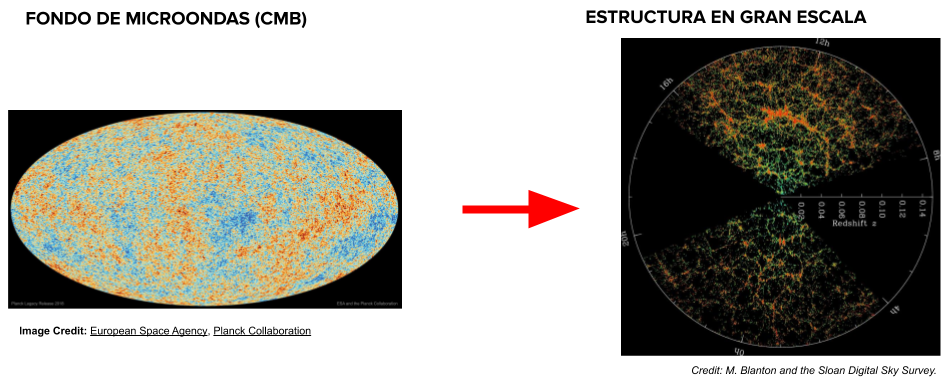
\includegraphics[width=10cm]{Figures/SeminarioII_agustin_rodriguez.png}
\decoRule
\caption[CMB]{Izquierda: Fondo de Microondas ($z\sim 3000$)}, imagen tomada de la colaboraci\'on Planck. Derecha: Universo cercano $(z\sim 0)$ de el cat\'alogo SDSS.
\label{CMB}
\end{figure}

La pregunta que surge es como hizo entonces el universo para pasar de ser altamente homogeneo a convertirse en un universo altamente inhomogeneo, dando lugar de esta manera a las galaxias y sistemas de estas. Y la respuesta a esta pregunta viene dada por las siguientes ecuaciones que describen la evolucion de las perturbaciones gravitatorias que, junto a otros procesos hidrodin\'amicos, generaron las estructuras que hoy en d\'ia conocemos como galaxias o c\'umulos. 

\begin{equation}
    \frac{\partial{\rho}}{\partial{t}}+\frac{3\dot{a}}{a}\rho+\frac{1}{a}\nabla.(\rho\textbf{u})=0
    \label{continuidad}
\end{equation}{}

\begin{equation}
    \frac{\partial{u}}{\partial{t}}+\frac{\textbf{u}.\nabla}{a}\textbf{u}+\frac{\dot{a}}{a}\textbf{u}=-\frac{1}{\overline{\rho}a}\nabla{P}-\frac{1}{a}\nabla{\Phi}
    \label{euler}
\end{equation}{}

\begin{equation}
    \nabla^{2}\Phi(\textbf{x},t)=4\pi Ga^{2}(t)\overline{\rho}\delta(\textbf{x},t)
    \label{poisson}
\end{equation}{}

\begin{equation}
    p=\omega \rho
    \label{estado}
\end{equation}{}

La ecuacion \ref{continuidad} es conocidad como la ecuaci\'on de continuidad, que expresa simplemente la conservaci\'on de la masa. La segunda ecuaci\'on, \ref{euler} es conocidad como ecuaci\'on de la conservaci\'on del momento o ecuaci\'on de Euler. Esta ecuaci\'on vectorial detalla el movimiento de las particulas, en el lado derecho tenemos un t\'ermino que responde a el potencial gravitacional $(\Fi$) y un termino que responde a la presi\'on ($P$). Estos gradientes son llamados \textit{terminos fuentes} de la ecuaci\'on de Euler. Si bien en esta formulacion solo se incluyen dos t\'erminos fuentes, pueden incluirse otras fuentes de fuerzas tales como campoes electromagn\'eticos.. etc. La ecuaci\'on \ref{Poisson} relaciona el potencial gravitacional generado por una distribuci\'on inhomogenea de materia ($\delta$) que depende del tiempo y de la posici\'on. Finalmente la ecuaci\'on \ref{estado} me relaciona a la presi\'on (p) con la densidad de materia ($\rho$) donde a diferentes tipos de materia (gas, materia oscura, etc) corresponden diferentes constantes $\omega$. 

%Para estudios cosmologicos es conveniente reescribir las ecuaciones \ref{continuidad} y \ref{euler} en t\'erminos de coordenadas en expansi\'on y en funci\'on de el contraste adimencional de densidad $\delta$ CITA PEEBLES, quedando entonces:

%\begin{equation}
%    \frac{\partial v}{\partial t} + \frac{1}{a}(\textbf{v} \cdot \nabla)\textbf{v} + \frac{\dot{a}}{a}\textbf{v}=-\frac{1}{\rho a}\nabla p - \frac{1}{a}\fi
%\end{equation}{}
%\begin{equation}
%    \frac{\partial \delta}{\partial t}+ \frac{1}{a}\nabla \cdot (1 + \delta )\textbf{v}=0
%\end{equation}{}



Como puede verse en el set de ecuaciones presentado, este constituye un sistema acoplado y altamente no lineal. La resoluci\'on entonces de estas ecuaciones para el estudio de la evoluci\'on de las perturbaciones de densidad es de gran dificultad y solo puede resolverse an\'aliticamente para casos que requieren un alto grado de simplificaciones y aproximaci\'on, para lo demas, es menester el uso de otras herramientas como las simulaciones num\'ericas, sobre las que no explayaremos en la siguiente secci\'on. 



\subsection{Teor\'ia de perturbaciones lineales}
\label{PerturbacionesLineales}

Un resultado an\'alitico para las ecuaciones que describen la evoluci\'on de las pertubaciones de densidad (\ref{continuidad},\ref{euler},\ref{poisson}) es posible al realizar un aproximaci\'on lineal, v\'alida para casos restringidos pero de suma importancia, como veremos m\'as adelante.


Consideraremos peque\~nas pertubaciones de densidad sobre un universo homog\'eneo ($\delta \ll 1 $). Para trabajar con las ecuaciones \ref{continuidad} \ref{euler} primero las escribiremos en t\'erminos de el contraste $\delta$ y luego consideraremos t\'erminos de primer orden en $\delta$ y \textbf{u}. De esta manera, manipulando algebraicamente las ecuaciones obtenemos las siguientes relaciones para la evoluci\'on del contraste de densidad \citep{ElPeebles}
\begin{equation}
 \frac{\partial^{2}\delta}{\partial t ^{2}}+ \frac{2 \dot{a}}{a}\frac{\partial \delta}{\partial t}=4\pi G   \overline{\rho}\delta 
 \label{EcuacionDeltaAproximacion}
\end{equation}

\begin{equation}
    \frac{\partial ^{2}{\delta}}{\partial t ^{2}}+ \frac{1}{a}\nabla \cdot \textbf{u}= 0
\end{equation}{}

Queda expl\'ito que la soluci\'on para el contraste $\delta$ no depende de la posici\'on (al menos para la aproximaci\'on lineal), por lo que las soluciones seran de la forma 
\begin{equation}
    \delta({\textbf{x},t})=D(t)S(\textbf{x})
\end{equation}{}

Bajo esta forma funcional, del hecho de que el contraste no tiene una dependencia espacial, se puede realizar una expansi\'on en el espacio de Fourier de las frecuencias espaciales donde el contraste de densidad $\delta$ adoptar\'ia la siguiente forma:

\begin{equation}
    \delta(\textbf{x})=\sum_{i=0}^{\infty} \hat{\delta}(\textbf{k}) e^{-i\textbf{k}\cdot \textbf{x}}
    \label{seriefourier}
\end{equation}{}

De modo que vemos que podemos representar al universo como una superposici\'on de ondas de diferentes fases, cuya amplitud viene dada por un espectro de potencias.
\begin{equation}
    P(k)=<\mid \hat{\delta}(k) \mid ^{2}>
\end{equation}{}



\section{Vac\'ios en la literatura}

La figura \ref{SDSS} presenta la distribuci\'on de galaxias del universo cercano obtenida por el proyecto \textit{Sloan Digital Sky Server}, conocido como SDSS. \textcolor{red}{CITA}. Pueden aprecirse como las regiones sobredensas del universo rodean zonas subdensas, conocidas como \textit{cosmic \textbf{voids}}. Estas regiones, pensadas taxonomicamente como una componente de la estructura en gran escala del universo, constituyen la mayor parte del contenido del universo \citep{Sheth2004}.

T\'ipicamente alcanzan contrastes de densidad de $\delta\simeq$-0.9. No existe un consenso en cuanto a la forma de estos, aunque la tendencia general es que se tornen estructuras esf\'ericas \citep{Sheth2004}. Lo mas facil es identificarlos con formas esf\'ericas, aunque tambi\'en pueden adoptarse otros criterios para esto. 

Existen diversos estudios realizados con c\'atalogos de diferentes relevamientos sobre las propiedades de las galaxias que habitan estos entornos subdensos. Estos carecen de galaxias brillantes y su estructura interna es trazada fundamentalmente por galaxias d\'ebiles \citep{Alpaslan2014}. En general, la din\'amica interna de los vac\'ios es expansiva \cite{Sheth2004} por lo que las galaxias dentro de estos ambientes siente una constante de hubble mayor. De esta manera la formaci\'on de estructuras dentro de los vac\'ios es mas lenta que en otro ambientes \citep{Kreckel2016} ? \cite{Tomita2000} . Esto otorga a las galaxias en voids propiedades muy caracteristicas. \citep{Ceccarelli2008} encuentra que estas son azules y con tasas altas de formaci\'on estelar. De modo que existe una modulaci\'on de la gran escala en estas propiedades astrof\'isicas que va mas all\'a de el entorno local. 




\begin{figure}
    \centering
    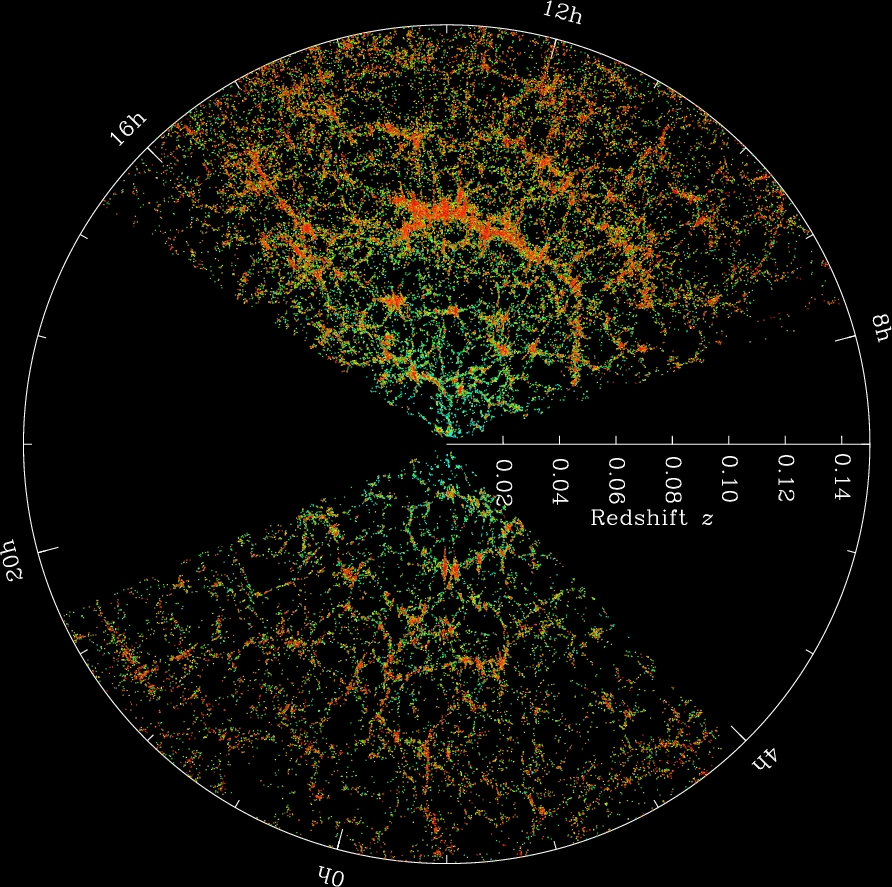
\includegraphics[width=10cm]{Figures/orangepie.jpg}
    \caption{Caption}
    \label{SDSS}
\end{figure}{}

%\section{Simulaciones Num\'ericas}
%Segun el paradigma del universo $\Lambda CDM$, la densidad de materia en el universo esta dominada por la materia oscura. Por lo cual, la din\'amica general del universo esta dominada por la din\'amica de la materia oscura, y la materia bari\'onica acompaña esta din\'amica, introduciendo efectos que, al menos en un principio, se espera que sean \textit{secundarios}. 
%De modo que una descripci\'on detallada de lo que le suceda a , por ejemplo, una galaxia requerir\'a de simular las interacciones de N-cuerpos de materia oscura. Si quisiera representarse cada estrella en una galaxia con una particula, esto requeria de $\sim 10^{10}$particulas, y estos n\'umeros son imposibles de simular, por lo cual, las t\'ecnias actuales requieren de algunas simplificaciones de los problemas. En particular, se discretiza las distribucion de materia considerando un n\'umero de particulas mucho menor al real. 

%\subsection{Ecuaci\'on de Bolzmann}

%La aproximaci\'on utilizada para resolver los problemas de N-cuerpos, requiere considerar a las particulas en un sentido estad\'istico. Cada part\'icula simulada representa entonces una poblaci\'on de part\'iculas f\'isicas (de estrellas, gas, materia oscura, etc.) con propiedades f\'isicas similares, es decir, casi posiciones identicas o velocidades. La evoluci\'on de estos ensambles de part\'iculas es gobernada entonces por la mec\'anica estad\'istica. 

%Podemos pensar al universo entonces como un \textit{fluido} descripto por las ecuaciones  de la hidrodin\'amica. El n\'umero de particulas dN, con posiciones entre \textbf{x + dx}, velocidades \textbf{u + du} en un tiempo t es entonces
%\begin{equation}
%    dN=f(\textbf{x}, \textbf{u}, t)\textbf{dx}\textbf{du}
%\end{equation}{}
%Un elemento de volumen que contenga un n\'umero suficientemente grande de part\'iculas podra ser tratado estad\'isticamente. Suponemos sus posiciones entre \textbf{x+dx} y con velocidades \textbf{u+du}, y consideremos un campo de fuerza \textbf{F} que no cambia apreciablemente con distancias comparables a la distancia media entre part\'iculas. Sea \textbf{q} el momento, tal que \textbf{q}=m\textbf{u}, entonces se encuentra que
%\begin{equation}
%    \frac{\partial{f}}{\partial{t}}+u_{i}\frac{\partial{f}}{\partial{}x_{i}}+F_{i}\frac{\partial{f}}{\partial{u_{i}}}=[\frac{\partial{f}}{\partial{t}}]_{col}
%\end{equation}{}
%Esta es conocida como la \textit{Ecuaci\'on de Boltzmann} y describe la evoluci\'on de una funci\'on distribuci\'on en el espacio de seis dimensiones (\textbf{x}.\textbf{u}) llamado espacio de fases.  Expresa el hecho de que el cambio en el n\'umero de particulas en un elemento de volumen del espacio de fases es igual a el n\'umero de particulas que entran o dejan el elemento. 



%\subsection{Condiciones Iniciales}

%\subsection{Metodos de integraci\'on}

%\subsection{SPH}


\chapter{Herramientas Numericas} % Main chapter title

\label{SN} % For referencing the chapter elsewhere, use \ref{Chapter1} 

%----------------------------------------------------------------------------------------

% Define some commands to keep the formatting separated from the content 


Las simulaciones num\'ericas constituyen una de las herramientas mas importantes para el desarrollo de la astronom\'ia moderna. La enorme cantidad de particulas que constituyen por ejemplo una galaxia, hacen que los estudios an\'aliticos se vuelvan practicamente imposible. En este contexto es que cobra importancia un enfoque num\'erico de ciertos problemas constituidos por sistemas de muchas particulas y a\'un en estos casos se realizan aproximaciones. 
Aquellos sistemas que puedan ser descriptos como un fluido no collisional, permiten que los problemas se simplifiquen al poder lidiar con un conjunto muy reducido de particulas, conservando el comportamiento general del sistema. Dentro de este tipo de \textit{fluidos}, tenemos a las galaxias, sistemas de galaxias y a la materia oscura. CITA (Chandrasekhar 1943):? (Saas Springel? ). Por lo tanto, las simulaciones numericas cobran vital importancia en cosmolog\'ia por la practicidad que presentan. 


En este capitulo presentaremos una introducciones a la realizaci\'on de simulaciones numericas. Como generar sus condiciones iniciales y c..

\section{Simulaciones Num\'ericas}

\subsection{Din\'amica de macro particulas}

El modelo actual del universo es el de $\Lambda$CDM. Bajo este paradigma la materia del universo esta compuesta en casi $\sim 80 \% $ de materia oscura, y un $\sim 20 \% $ de materia bari\'onica. De modo que es esperable que la din\'amica general del universo este gobernada por lo que suceda con la materia oscura y que los bariones \textit{acompa\~nen} a la din\'amica de la materia oscura. 




Aca la idea es contar que en los fluidos no colisionales, como puede ser un universo descripto por materia oscura, un conjunto de macro particulas se comportan segun la ecuacion de Boltzman (desde donde se pueden recuperar las ecuaciones hidrodin\'amicas qeu voy a poner en la introduccion.)

Aca hacer una diferenciacion de cuando uno trabaja con particulas de gas o de materia oscura la integraci\'on va a ser diferente. 




\subsection{Condiciones Iniciales}
Tal como se vio en la secci\'on \ref{PerturbacionesLineales} la ecuaci\'on \ref{seriefourier}  nos permite representar a el contraste de densidad del universo como una superposici\'on de ondas de Fourier cuya amplitud viene dada por un espectro de potencias. Este espectro nos caracteriza el nivel de fluctuaciones a una dada escala espacial y puede medirse atrav\'es de relevamientos de galaxias. 

Generar condiciones iniciales para una simulaci\'on, consiste entonces en reproducir mediante una distribuci\'on de particulas el estado del universo temprano, para luego integrar las ecuaciones de movimiento de estas particulas, evolucionando asi el universo desde un estado temprano a alto redshift a el universo tal como lo conocemos hoy. 

De modo que en general, se utiliza la teor\'ia de perturbaciones lineales para generar el nivel de perturbaciones inicial, ya que a un redshift suficientemente alto, el universo a\'un estar\'ia en un r\'egimen lineal y ser\'ia v\'alida esta aproximaci\'on. Se generan entonces perturbaciones que tienen una amplitud conocida por el espectro de potencias pero una fase aleatoria. El hecho de qu eno podamos medir las fases de las perturbaciones del universo real hace que no podamos simular el universo real que habitamos. Por lo cual es importante resaltar que las simulaciones no constituyen una materializaci\'on del universo \textit{real}, sino que uno simula universos \textit{estad\'isticamente similares}. 

\subsection{Aproximaci\'on Zeldovich}

Podemos entonces escribir a las fluctuaciones de densidad en el espacio de Fourier donde entonces la fluctuacion en una escala k es:
\begin{equation}
    \hat{\delta}(k)=\delta_{k}e^{i\fi_{k}}
    \label{PerturbacionEscalaK}
\end{equation}{}
Donde la probabilidad de tener una fluctuaci\'on con una cierta fase y amplitud sigue una distribuci\'on exponencial en el cuadrado de $\delta_{k}$ y uniforme en la fase \textbf{Cita libro carlos}:
\begin{equation}
    P(\delta_{k},\phi_{k})=\frac{1}{2\sigma_{k}^{2}\pi}exp{(-\frac{\delta_{k}^{2}}{\sigma_{k}^{2}})^{2}}\delta_{k}d(\delta_{k}^{2})d\phi_{k}
  \label{ProbabilidadFluctuaciones}
\end{equation}{}
\begin{equation}
    \sigma_{k}^{2}=<\mid \hat{\delta}_{k}^{2} \mid >=P(k)
\end{equation}{}
Si uno escribe la perturbaci\'on \ref{PerturbacionEscalaK} como $\delta(k)=a_{k}+i b_{k}$ se puede demostrar que la ecuaci\'on \ref{ProbabilidadFluctuaciones} se transforma en una distribuci\'on Gausseana para $a_{k}$ y $b_{k}$ \textbf{cita libro carlos DODELSON}. Observaciones de el CMB \textbf{cITA?} permiten ver que las fluctuaciones de este son gauseanas, dando sustento a la teor\'ia. Al mismo tiempo, esta probabilidad de fluctuaciones esta predecida por las teor\'ias modernas de inflaci\'on. 

\begin{figure}
    \centering
    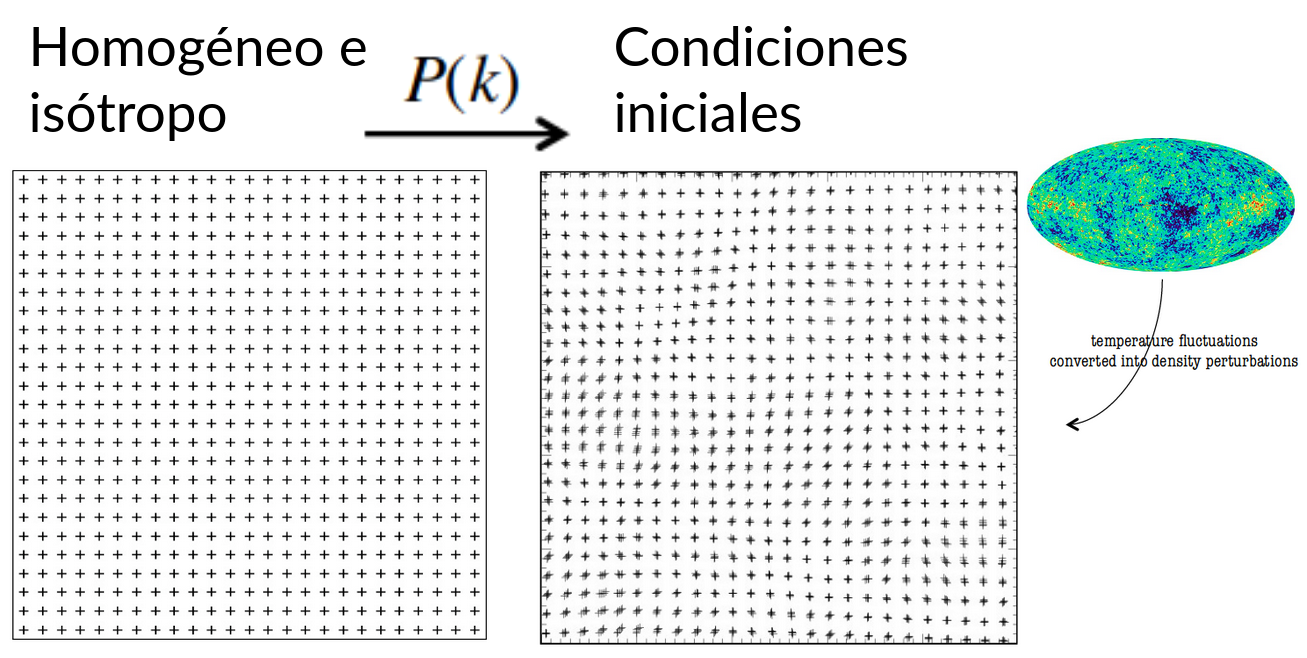
\includegraphics[width=12cm]{Figures/Captura de pantalla de 2020-01-11 16-26-38.png}
    \caption{\textbf{EDITA UNA IMAGEN CON ESTA ONDA. CITALO A KNEBE}}
    \label{Knebe}
\end{figure}{}

Lo que queremos hacer entonces es a partir de una distribuci\'on homogenea de particulas obtener una distribuci\'on que este levemente perturbada, cuyas fluctuaciones de densidad sean representativas de las de un universo temprano (figura \ref{Knebe}. Para esto se utiliza la \textit{Aproximaci\'on Zeldovich} \citep{Zeldovich1970}.

Esta consiste en obtener las posiciones $\textbf{x}(t)$ (denominadas posiciones eulerianas) a partir de las posiciones $\textbf{q}$ en una grilla homog\'enea (denominadas posiciones lagrangianas). La aproximaci\'on toma la forma dada por:

\begin{equation}
    \textbf{x}(t)=\textbf{q}+D(t)\textbf{S}(\textbf{q}) 
    \label{Zeldovich}
\end{equation}{}

La ecuaci\'on \ref{EcuacionDeltaAproximacion} se puede resolver num\'ericamente para obtener el valor de D(t). Esto es lo que comunmente se denomina \textit{Growth Factor} (Factor de crecimiento) que nos indica como se expande el universo con el tiempo y es una funci\'on que depende de la cosmolog\'ia que uno utilice.

El campo de desplazamiento \textbf{S}(\textbf{q} podemos escribirlo como el gradiente de un potencial \citep{Zeldovich1970}, y se puede demostrar que este potencial viene dado, a menos una constante, por las fluctuaciones de densidad $(\delta_{0})$. Entonces tenemos lo siguiente: 
\begin{equation}
    \textbf{S}(\textbf{q})=-\nabla\Psi
    \label{CampoS}
\end{equation}{}
\begin{equation}
    \nabla ^{2}\Psi=\delta_{0}
\end{equation}{}

En el espacio de Fourier esta ultima ecuaci\'on adopta una forma muy simple de:

\begin{equation}
    \hat{\Psi}=\frac{\hat{\delta}_{0}(k)}{k^{2}}
    \label{Transformadadelcampo}
\end{equation}{}

Tenemos entonces ahora todos los elementos para generar condiciones iniciales para una simulaci\'on. En resumen los pasos son los siguientes:
\begin{itemize}
    \item Dado un espectro de potencias P(k) voy a tener las amplitudes de las fluctuaciones a diferentes escalas espaciales.
    \item Vimos como son las probabilidades de obtener fluctuaciones de diferentes escalas, y si escribo $\delta(k)=a_{k} + i b_ {k}$ las probabilidades de $a_{k}$ y $b_{k}$ dependen de generar numeros aleatorios que sigan una distribuci\'on Normal.
    \item Habiendo generado las fluctuaciones puedo simplemente obtener el campo $\hat{Psi}$ siguiendo la ecuacion \ref{Transformadadelcampo}.
    \item Lo siguiente es antitransformar $\hat{\Psi}$ para obtener el campo en el espacio real $\Psi$.
    \item Y tomando el gradiente de este campo obtengo el campo de desplazamiento \textbf{S}. \ref{CampoS}
\end{itemize}{}

Las velocidades iniciales se obtienen facilmente derivando la ecuaci\'on \ref{Zeldovich}.
\begin{equation}
    \dot{\textbf{x}}=\dot{D}\textbf{S}(\textbf{q})
\end{equation}{}

\subsection{Limitaciones}
\label{Limitaciones}
Este m\'etodo tiene limitaciones que deben ser tenidas en cuenta a la hora de llevarlo a la practica. Estas son dos y vienen dadas por la cantidad de particulas que uno desee simular y por el tama\~no del \textit{box} cosmol\'ogico que uno utilice.

\begin{figure}
    \centering
    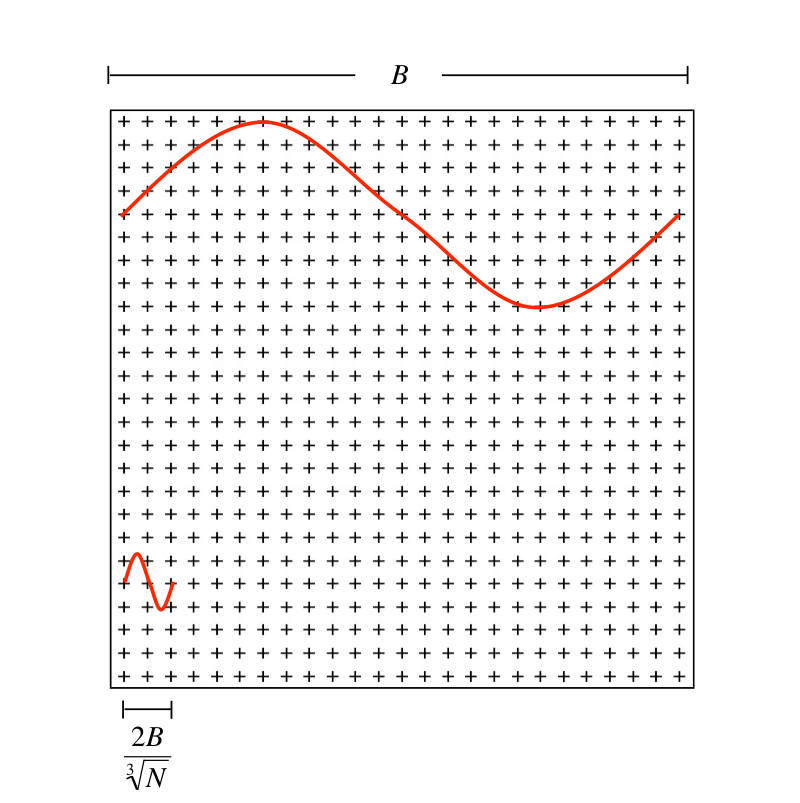
\includegraphics[width=12cm]{Figures/Captura de pantalla de 2019-10-02 17-37-57.png}
    \caption{Caption}
    \label{fig:my_label}
\end{figure}{}

Debido a que estamos reproduciendo una funci\'on en el espacio de fourier, las frecuencias mas largas que podemos reproducir vienen delimitadas por la regi\'on de periodicidad, que en nuestro caso es el tama\~no del \textit{box} que simulemos. 

Por otro lado, las frecuencias mas cortas que podamos reproducir estan delimitadas por el criterio de Niquist, y esto sera inversamente proporcional a la distancia media entreparticulas $^{3}\sqrt{N}$. Entonces cuantas mas particulas uno simule, la frecuencia de Niquist sera mas corta y asi podre simular frecuencias mas cortas. 


\subsection{Simulaci\'on}

Hasta aqu\'i hemos explicado como generar condiciones iniciales para una simulaci\'on. Estas condiciones iniciales comprenden a las posiciones y velocidades iniciales de las particulas. Lo siguiente entonces es integrar estas ecuaciones, para lo cual se utilizan c\'odigos de N-cuerpos. 

En el caso de que solo se simulen particulas de materia oscura, esta se movera solo por el campo gravitatorio generado por todas ellas. Este campo gravitatorio genera una potencial gravitatorio que genera a su vez una fuerza. Existen diversos m\'etodos para calcular los potenciales gravitarios, algunos de ellos son el \textit{particula-particula, Particle Mesh, TreePm, tecnicas de Fourier, etc.} 
Una elegante discusion de los diferentes m\'etodos es dada por \citet{SAAS}. 

\begin{figure}
 \centering
  \subfloat[Gatito]{
   \label{f:gato}
    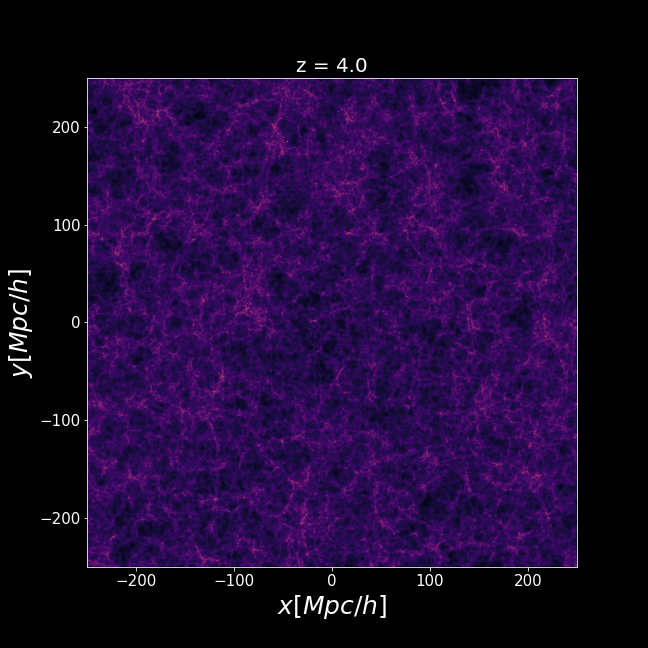
\includegraphics[width=0.3\textwidth]{Figures/base2.png}}
  \subfloat[Tigre]{
   \label{f:tigre}
    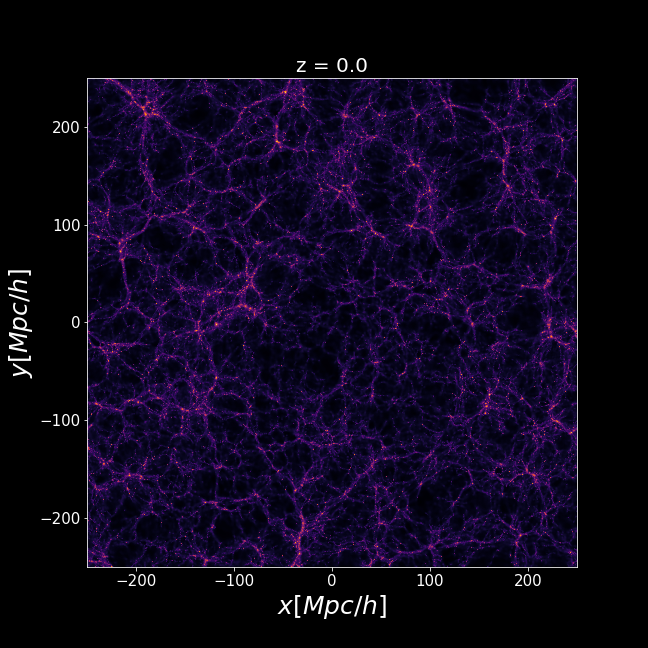
\includegraphics[width=0.3\textwidth]{Figures/base8.png}}
  
 \caption{Múltiples imágenes}
 \label{f:animales}
\end{figure}
 


\section{F\'isica Bari\'onica}

Los procesos astrof\'isicos que le ocurre a la materia barionica son de una enorme complejidad y dependen de una ampl\'isima gama de escalas. Por lo que implementarlos en un c\'odigo num\'erico requiere de un buen grado de model\'istica que var\'ia con las escalas que uno quiera estudiar. 

Principalmente en el universo los bariones se encuentran en estado gaseoso. A diferencia de la materia oscura, el gas se mueve no solo dominado por la gravedad sino que tambi\'en lo hace debido a los gradientes de presi\'on que generan fuerzas. Si queremos integrar entonces las ecuaciones de movimiento no solo de particulas de materia oscura, sino que tambi\'en particulas de gas, esto presenta una primera dificultad, ya que debemos ser capaces de generar a partir de particulas discretas campos \textit{continuos}, que puedan ser derivados para calcular propiedades (como la presi\'on). Existen diversas maneras de hacer esto, una de las mas importantes es lo que se conoce como \textbf{Smooth particle hidrodynamics} (\textit{SPH}) o en espa\~nol, \textit{Hidrodin\'amica de particulas suavizadas}.

\subsection{Hidrodin\'amica de particulas suavizadas}
\label{SPH}

\citet{Gingold1977} desarrollaron una manera de representar propiedades continuas de fluidos atrav\'es del uso de particulas. Esta t\'ecnica que originalmente se penso para el uso de c\'odigo magnetohidrodin\'amicos, pronto se popularizaron para el uso de calculos astrof\'isicos. La idea es simple y consiste en interpolar las propiedades en el espacio mediante el uso de un \textit{Kernel}. Se representa entonces cualquier campo \textbf{F}(\textbf{r} de la siguiente manera:
\begin{equation}
    \textbf{F}(\textbf{r})=\int \textbf{F}(\textbf{r}')W(\textbf{r}-\textbf{r}',h)d\textbf{r}'
    \label{IntegralSPH}
\end{equation}{}

La funci\'on W es el \textit{Kernel Interpolatorio}, normalmente se utilizan funciones de soporte compacto, como un spline c\'ubico. La variable h es el \textit{ancho} del kernel. Para ser factible implementar este m\'etodo en un c\'odigo num\'erico debemos discretizar la integral \ref{IntegralSPH}. Para particulas con una masa $m_{i}$ y una densidad $\rho_{j}$ podemos asignarles un \textit{volumen caracteristico} $V_{i}\sim m_{j}/\rho_{j}$ que utilizaremos como diferencial de volumen, entonces la ecuacion \ref{IntegralSPH} se aproxima de la siguiente manera:
\begin{equation}
    \textbf{F}(\textbf{r})\simeq \sum_{j} \frac{m_{j}}{\rho_{j}} F_{j} W(\textbf{r}-\textbf{r}_{j},h)
    \label{IntegralSPHDiscreta}
\end{equation}{}

\ref{IntegralSPHDiscreta} es una integral en el sentido \textit{Monte Carlo}. Para tener una buena estima de el valor del campo \textbf{F} en el punto \textbf{r} un debe efectuar la suma sobre una cantidad adecuada de particulas. Por supuesto que la mejor estima se obtiene al realizar la suma sobre todas las particulas, pero esto es num\'ericamente costoso. Realizar la suma sobre una cantidad $n\sim30$ genera una buena estima del campo. C\'odigos mas modernos como \texttt{\textbf{GIZMO}} la realizan sobre las 56 vecinas mas cercanas \citep{GIZMO2015}.

Por ultimo, para realizar la interpolaci\'on la variable h de el \textit{Kernel} W normalmente es la distancia a la n-\'esima vecina mas cercana. El \textit{Kernel} es tal que si $h\rightarrow 0$ $W \rightarrow \delta_{dirac}$, esto produce que una determinada propiedaded este localizada en un entorno peque\~no, mientras que si h es \textit{grande} las propiedades se distribuyen ampliamente en el espacio. 

\subsection{Modelos Astrof\'isicos \textit{Subgrid}}

La t\'ecnica de SPH, asi como otros m\'etodos como el particle mesh, adaptative mesh \textbf{CITAS} permiten integrar las ecuaciones de particulas de gas y de esta manera seguir su din\'amica. Ahora bien, procesos sumamente complejos producen que los bariones colapsen y formen nebulosas, a su vez estas formen estrellas que luego explotan como supernovas, estas aumentan la temperatura del gas circundante, se forman agujeros negros, y muchisimos otros procesos que ocurren a escalas mucho mas all\'a de las que pueden resolver las computadoras mas modernas. Debido entonces a que interacciones de estas escalas no pueden resolverse directamente en simulaciones cosmologicas se implementan otras alternativas para poder estudiar las propiedades bari\'onicas del universo.

Para poder reproducir fen\'omenos astrof\'isicos en simulaciones cosmologicas se implementan lo que se conoce como modelos \textit{sub-grid}. La idea es reproducir fen\'omenos que ocurren mas all\'a de el nivel de resoluci\'on de la simulaci\'on. Estos modelos reproducen en un sentido estad\'istico las propiedades barionicas del universo. 

La cantidad de modelos es muy ampl\'ia y abarca una amplia gama de complejidad. Aqu\'i se explican los principios b\'asicos sobre los que se calculan propiedades bari\'onicas en el modelo de \citet{Springel2003}.
La idea es que las particulas de SPH tienen una \textit{parte} de poblaci\'on condensada (c) que se encuentra en presi\'on de equilibrio y otra \textit{parte} caliente (h). Las nubes frias o poblaci\'on condensada proveen el material disponble para la formaci\'on estelar. En estas particulas \textit{hibridas} solo la poblaci\'on caliente esta sujeta a las ecuaciones d ela hidrodin\'amica. La parte fria interactua bajo gravedad pero si participa en los intercambios de energ\'ia y masa con la fase caliente. De modo que la densidad total de una particula de gas es la suma de las densidades de las dos poblaciones. 
\begin{equation}
    \rho = \rho_{h} + \rho_{c}
\end{equation}{}
Se modelan entonces 3 procesos que intercabian masa y energ\'ia entre las 2 fases.
\begin{itemize}
    \item \textbf{Formaci\'on Estelar}: 
    \begin{equation}
        \frac{d{\rho_{\star}}}{d{t}}=\frac{\rho_{c}}{t_{\star}}-\beta\frac{\rho_{c}}{t_{\star}}
    \end{equation}{}
    $t_{\star}$ representa un tiempo caracteristico en que las nubes fr\'ias convierten estrellas y $\beta$ es la fracci\'on de las estrellas m\'asivas que se forman. Estas estrellas tienen tiempos de vida muy cortos e instant\'aneamente explotan como supernovas. Tanto $\beta$ como $t_{\star}$ son par\'ametros del modelo. Notese que la fracci\'on $\beta$ que produce supernovas va a generar instant\'aneamente un intercambio de energ\'ia mediante \textit{feedback}. 
    
    \item \textbf{Calentamiento por \textit{feedback}}
    \begin{equation}
    \frac{d}{dt}(\rho_{h}u_{h})|_{SN}=\epsilon_{SN}\frac{d\rho_{\star}}{dt}=\beta u_{SN}\frac{\rho_{c}}{t_{\star}}
    \end{equation}{}
    
    $\epsilon_{SN}$ es la cantidad de energ\'ia que libera una supernova y es otro par\'ametro del modelo. El calentamiento producido por las supernovas lo que va a producir es un aumento de la energ\'ia interna (u) de las particulas cercanas, calentando de esta manera la fase caliente de las particulas.
    
    Este aumento de temperatura va a producir que las nubes fr\'ias se evaporen, retornando de esta manera material a la fase caliente. 
    \begin{equation}
        \frac{d\rho_{c}}{dt_{\star}}=A\beta\frac{\rho_{c}}{t_{\star}}
    \end{equation}{}
    donde A es la eficiencia de evaporaci\'on y tambi\'en constituye un par\'ametro del modelo. 
    
    \item \textbf{Crecimiento de nubes frias}: 
    \begin{equation}
        \frac{d\rho_{c}}{dt}|_{TI}=-\frac{d\rho_{h}}{dt}|_{TI}=\frac{1}{u_{h}-u_{c}}\Lambda_{net}(\rho_{h},u_{h})
    \end{equation}{}
    La fase caliente va a producir procesos radiativos que van a producir un enfriamiento (\textit{cooling}) generando de esta manera que el gas caliente se transforme en gas frio. Este proceso va a depender de la \textit{Funci\'on de cooling} $\Lambda_{net}$ que uno implemente. 
    
\end{itemize}{}

As\'i de esta manera el modelo lo que produce es un intercambio entre las fases de gas que es autoregulatorio y reproduce estad\'isticamente propiedades astrof\'isicas del universo. En un esquema general, cuando la poblaci\'on de gas fr\'io sea lo suficientemente grande se formaran estrellas. Estas produciran supernovas que reinsertaran energ\'ia al ambiente por \textit{feedback} calentando de esta manera el gas. Este gas caliente comenzara a radiar y de esta manera se enfriara, aumentan la poblaci\'on caliente, y el ciclo se reanuda. 

El esquema aqui presentado es el correspondiente a \citet{Springel2003} y constituye uno de los mas simples modelos subgrid. Existen muchisimos modelos que reproducen otros fen\'omenos que aqu\'i se ignoran como por ejemplo la formaci\'on de agujeros negros supermasivos \textcolor{red}{textbf{BUSCAR CITA}} introduciendo otros tipos de feedback mas complejos. 

\section{Re-simulaciones }

En la secci\'on \ref{Limitaciones} se indico cuales eran las limitaciones que existen a la hora de realizar simulaciones y estas eran el tama\~no del \textit{box} y la cantidad de particulas que se utilicen. Si uno obtiene en un \textit{box peque\~no} una cantidad \textit{grande} de particulas, uno va a tener una simulaci\'on de mucha resoluci\'on. La resoluci\'on se refiere a la masa de las particulas que uno tenga, si esta masa disminuye entonces uno gana resoluci\'on, ya que va a poder muestrear una misma estructura con mas particulas, ganando asi detalles. 

Entonces si uno quiere hacer una simulaci\'on con mucha resoluci\'on va a tener que poner la mayor cantidad de particulas que pueda en su \textit{box}. Esto va a generar un problema ya que cuanto mas particulas uno quiera simular, mayor sera el tiempo de computo que uno requiera para integrar sus ecuaciones de movimientos. Existen situaciones en cambio en que a uno puede interesarle tener mucha resoluci\'on en tan solo una regi\'on de el \textit{box} y poca en otra. En estos casos se utiliza la t\'ecnica de \textit{Re-simulaciones} o simulaciones \textit{Zoom-in}. Por ejemplo uno querr\'ia simular un cumulo, y tener mucha resoluci\'on en la galaxia central y el resto de las galaxias miembros del grupo tenerlas solo para que ejerzan efectos tidales sobre la central. 

En general, la resimulaci\'on consiste en identificar en una simulaci\'on una regi\'on que a uno le interese, y luego volver a realizar la simulaci\'on pero obteniendo mas resoluci\'on en esa regi\'on. Entonces realizar una re-simulacion consta de al menos dos etapas. Primero se genera una simulaci\'on \textit{base} y luego se realiza al re-simulaci\'on en todo el \textit{box} original, con mayor resoluci\'on en alguna regi\'on. 

Para poder realizar esto, uno tiene que a las condiciones iniciales de la simulaci\'on \textit{base} agregarle perturbaciones de escalas mas chicas. En la regi\'on de inter\'es se agregan al mismo tiempo mas particulas disminuyendo asi la distancia media entre particulas. De esta manera en esta regi\'on las particulas seran sensibles a las nuevas perturbaciones que se agregaron en las condidiones iniciales.

Luego se vuelven a integrar las ecuaciones de movimientos de todas las particulas y el resultado final es la obtenci\'on de mayor resoluci\'on en la regi\'on de inter\'es. 




\begin{figure}
 \centering
  \subfloat[Gatito]{
   \label{f:gato}
    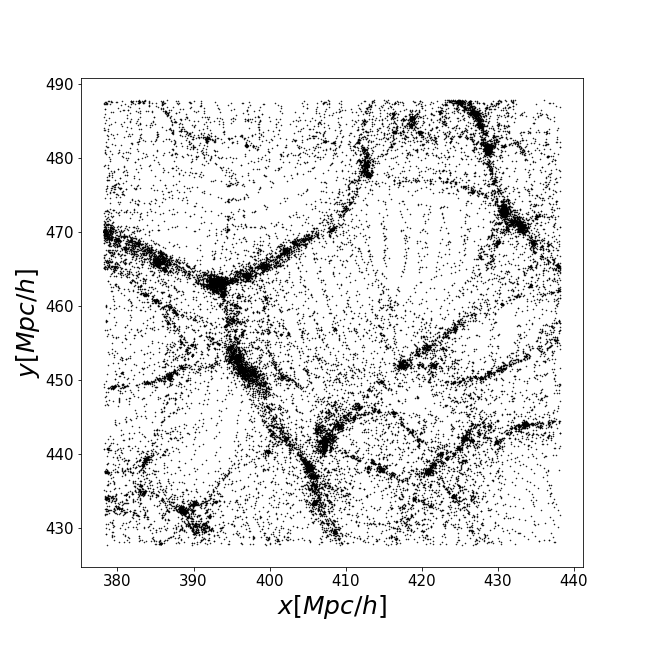
\includegraphics[width=0.3\textwidth]{Figures/proceso1.png}}
  \subfloat[Tigre]{
   \label{f:tigre}
    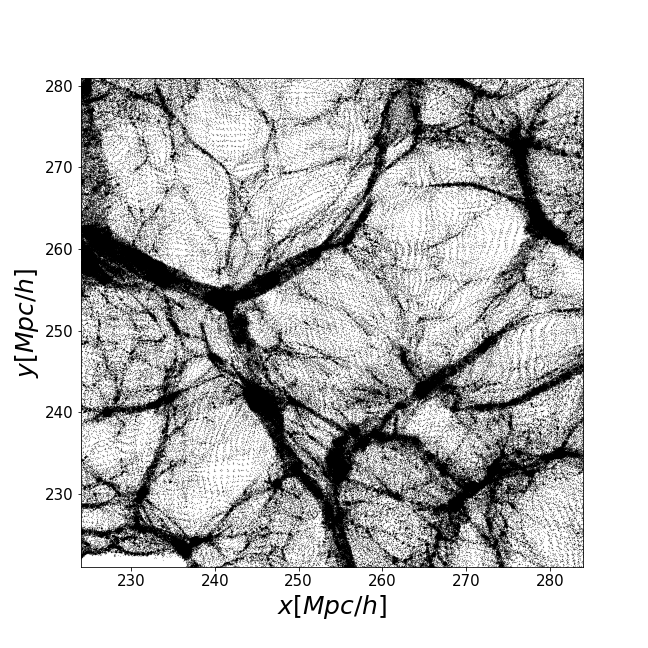
\includegraphics[width=0.3\textwidth]{Figures/proceso6.png}}
  
 \caption{Múltiples imágenes}
 \label{Resimulacion}
 
\end{figure}
 

La figura \ref{Resimulacion} presenta una simulaci\'on zoom-in realizada sobre un \textit{box} de 500 Mpc de lado. La imagen de el lado derecho es la resimulacion de la regi\'on de inter\'es (izquierda). Se puede observar que la resoluci\'on alcanzada es de mayor grado permitiendo de esta manera obtener mayor nivel de detalle. Pero en terminos generales las estructuras son las mismas, solo que con resouciones diferentes. 



\section{Halos de materia oscura}

Las particulas de materia oscura forman estructuras virializadas que se conocen como \textbf{halos}. Es en estas regiones donde los bariones colapsan para formar las galaxias. Por lo cual las estructuras trazadas por halos de materia oscura en las simulaciones deben ser an\'alogas a aquellas trazadas por galaxias. Existen diversos c\'odigos num\'ericos que identifican los halos en simulaciones y estos se construyen sobre diferentes fundamentos te\'oricos. A lo largo de este trabajo utilizaremos el c\'odigo \texttt{ROCKSTAR} desarrollado por \citet{Rockstar}  para la identificaci\'o de los halos de materia oscura en las simulaciones. Es importante destacar que este c\'odigo solo trabaja sobre las particulas de materia oscura. 


\section{Identificaci\'on}

Para identificar vac\'ios existen diferentes criterios, nosotros utilizamos el m\'etodo de \citep{Ruiz2015} donde los voids se definen como estructuras esf\'ericas cuyo contras de densidad integrado, definido por:
\begin{equation}
    \Delta(r)=\frac{3}{r^{3}}\int_ {0}^{r}\delta(r')r'^{2}dr'
    \label{ContrasteDensidadIntegrada}
\end{equation}{}
es de $\Delta=-0.9$.

El algoritmo trabaja de la siguiente manera:
\begin{itemize}
    \item Se comienza realizando una teselaci\'on de Voronoi sobre el cat\'alogo de halos o galaxias. Esta teselaci\'on consiste en calcular para cada punto trazador (halos) la regi\'on que esta mas cerca de este que de otro trazador.
    \item Se estima el campo de densidad, que consistira en $\rho_{celda}=\frac{1}{area celda}$. 
    \item Luego se eligira como candidatos a voids aquellas celdas que contengan una $\delta_ {celda}<-0.8$
    \item Se calcula el contraste de densidad integrada \ref{ContrasteDensidadIntegrada} en esferas alrededor de los trazadores seleccionados, hasta que alcancen $\Delta=-0.9$
    \item Mediante una caminata aleatoria alrededor de los trazadores se relocaliza un nuevo centro, desde donde se comienza a integrar el contraste $\Delta$ nuevamente. Si este alcanza $\Delta=-0.9$ a un radio mayor, se lo fija como nuevo centro.
    
\end{itemize}{}
De esta manera se hace iterativamente hasta lograr convergencia. 
\chapter{Resimulaciones de Vacios Cosmol\'ogicos} % Main chapter title

\label{Voids} %



\section{Simulaci\'on Base}

Se realiz\'o una simulaci\'on \textit{base} de solo materia oscura en un \textit{box} cosmologico de 500 Mpc de lado con $512^{3}$ particulas. Para esto se utiliz\'o el c\'odigo \texttt{\textbf{MUSIC}} \citep{MUSIC} para la generaci\'on de condiciones iniciales (a z=50) mientras que la integraci\'on se llevo al cabo con el c\'odigo \texttt{\textbf{GIZMO}} \citep{GIZMO2015}. 

Sobre esta simulaci\'on se identificaron los halos de materia oscura utilizando el identificador de halos \texttt{\textbf{ROCKSTAR}} \citep{Rockstar}. 

La figura \ref{Base2snap} presenta dos \textit{snapshots} de la misma, uno a z=4 y otro a z=0. Podemos observar como la estructura evoluciona claramente a medida que pasa el tiempo. La simulaci\'on a z=4 presenta un universo mucho mas homog\'eneo que a z=0. Las regiones donde se vislumbra alguna sobre densidad o subdensidad en la primera, son muy amplificadas a z=0 contituyendo grandes vac\'ios o filamentos o nodos de mucha densidad. 


\begin{figure}
    \centering
    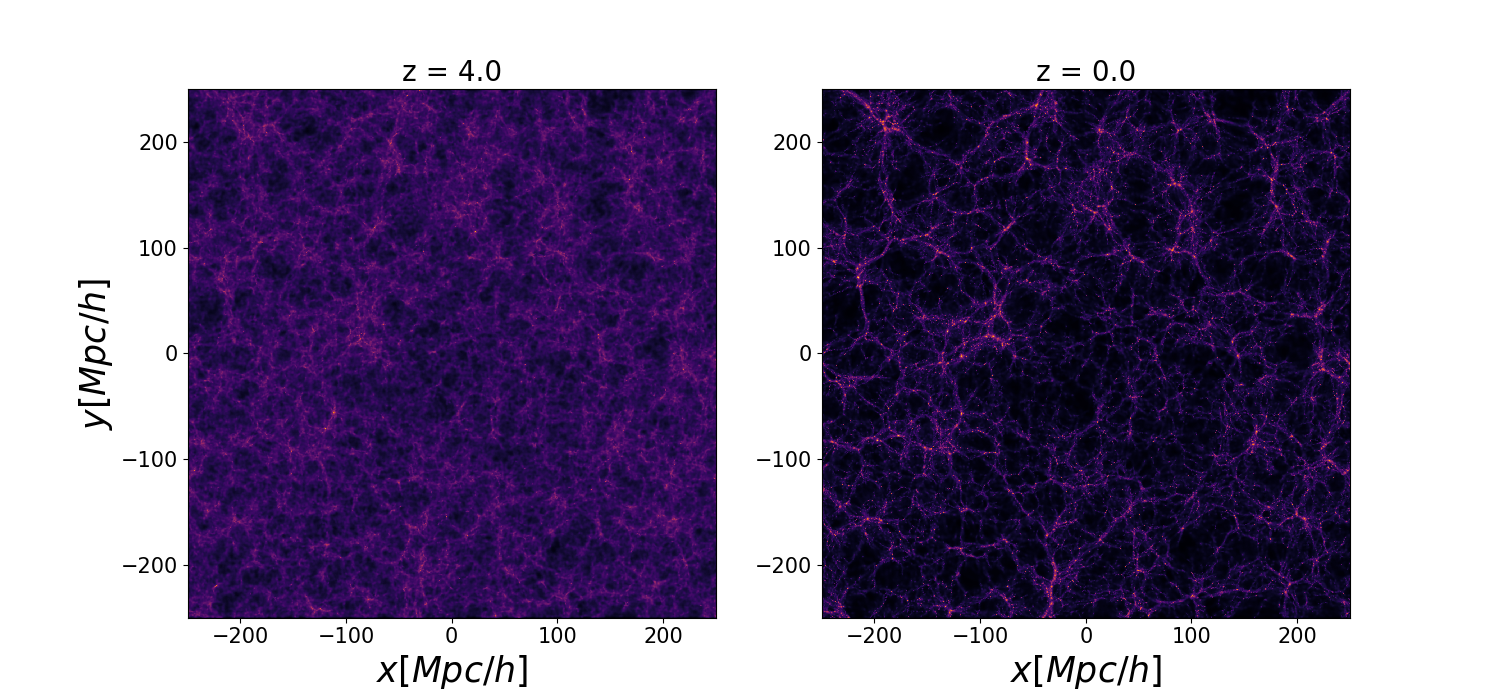
\includegraphics[width=15cm]{Figures/Base_2snap.png}
    \caption{Caption}
    \label{Base2snap}
\end{figure}{}

Tal como se menciono en la secci\'on \textbf{ALGUNA} la zonas de mas alta densidad atraen la materia por medio de su intenso potencial gravitacional. Con motivo de ilustrar este comportamiento se identifico una regi\'on de alta densidad y se calculo el campo de velocidad de el entorno. Esto se muestra en la figura \ref{Streamlines} donde podemos ver como las l\'ineas de campo de velocidad se dirigen hacia las zonas mas oscuras que corresponden a regiones de alta densidad. En la escala de colores de las l\'ineas se representa la intensidad de la velocidad. Se aprecia entonces que el campo alcanza su mayor intensidad en las proximidades de las zonas densas, siendo menores en los centros subdensos. 

\begin{figure}
    \centering
    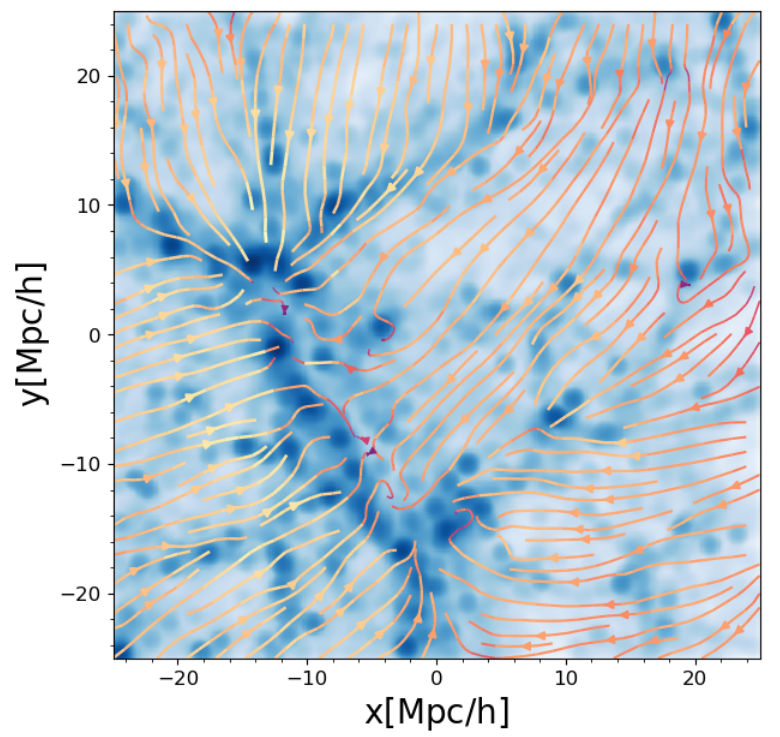
\includegraphics[width=13cm]{Figures/Streamlines.png}
    \caption{Caption}
    \label{Streamlines}
\end{figure}{}

\section{Identificaci\'on de Vac\'ios}

Con el algoritmo descripto en la secci\'on se identificaron los voids utilizados sobre la simulaci\'on \textit{base} utilizando el cat\'alogo de halos con un corte en 20 particulas. Los voids identificados entonces corresponden a los trazados por halos de $1.4$ $10^{12}M_{\odot}$. Sobre este cat\'alogo se identificaron 1384 voids. 
La figura \ref{VoidsIdentificados} es un corte transversal de la simulaci\'on donde las esferas marcan algunos de los voids identificados en la simulaci\'on. 

\begin{figure}
    \centering
    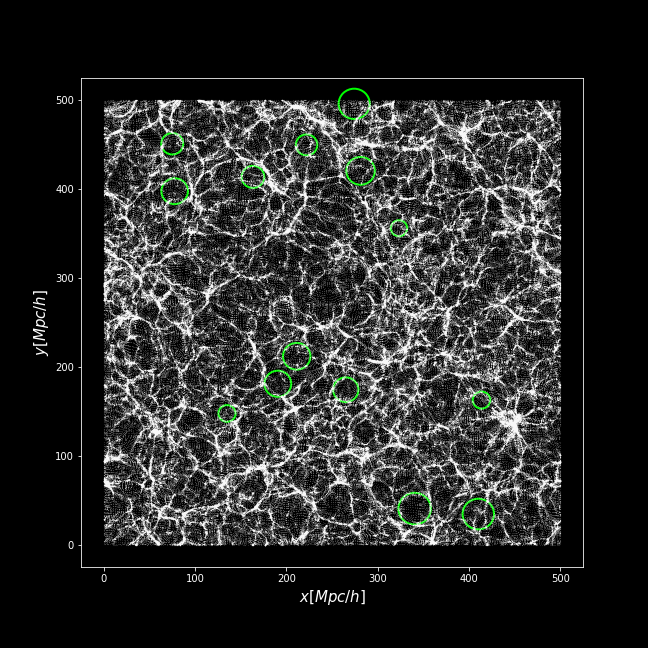
\includegraphics[width=12cm]{Figures/voids_r2.png}
    \caption{Caption}
    \label{VoidsIdentificados}
    
\end{figure}{}

Con el cat\'alogo de voids construido se contruyeron los perfiles de densidad integrada que pueden verse en la figure \ref{PerfilesVoids}. Cuando se observan los perfiles $\Delta$ los voids tienen dos tipos de comportamiento. Aquellos que alcanzan una $\Delta$ superior a la media del universo ($\Delta=0$) para luego decrecer hasta estabilizarse, y aquellos que crecen en $\Delta$ lentamente. Los primeros son los denominados voids \textbf{Tipo S} y los segundos los denominados \textbf{Tipo R}. Los tipo S presentan paredes muy sobredensas que se encuentran en proceso de colapso, esto produce que t\'ipicamente sean mas chicos que los tipo R \citep{Ceccarelli2013}.
\begin{figure}
    \centering
    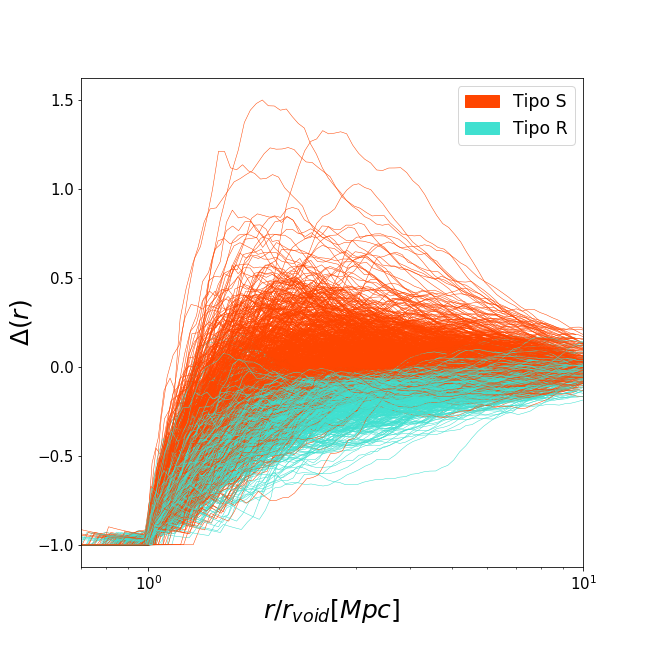
\includegraphics[width=12cm]{Figures/voids_sep.png}
    \caption{Caption}
    \label{PerfilesVoids}
\end{figure}{}

De la muestra de $\sim$ 1300 voids se seleccionaron 2, uno tipo S y uno R. Los perfiles de los voids seleccionados se presentan en la figura \ref{perfileshalos}. 

\begin{figure}
    \centering
    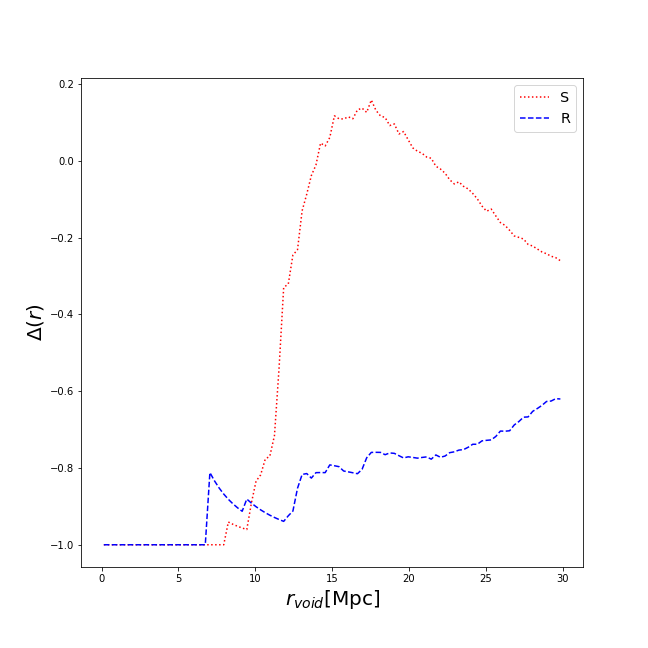
\includegraphics[width=\linewidth]{Figures/perfiles_halos.png}
    \caption{Caption}
    \label{perfileshalos}
\end{figure}{}

\section{Voids Resimulados}

Sobre el cat\'alogo de voids construidos se resimularon 2 vac\'ios, agregando particulsa de gas y recetas de \textit{feedback} y formaci\'on estelar siguiendo el modelo de \citet{Springel2003}. Un void tipo S y otro tipo R. Estos fueron seleccionados de modo que sean \textit{muy S y R} para de esta manera sean lo mas representativos posibles de la poblaci\'on general de cada tipo. Tanto la simulaci\'on \textit{base} como las resimulaciones fueron realizadas con el c\'odigo p\'ublico \texttt{\textbf{GIZMO}} \citep{GIZMO2015} y las condiciones iniciales iniciales se generan con el c\'odigo \texttt{\textbf{MUSIC}} \citep{MUSIC}. En la tabla \ref{Simulaciones0} del ap\'endice se presentan los datos de las simulaciones y resimulaciones utilizadas para este trabajo. 

En la figura \ref{Resi} se compara la regi\'on original de la simulaci\'on \textit{base} con su resimulaci\'on. Solo estamos representando particulas de materia oscura. Ambas son un corte transversal de 4 Mpc. Se observa que la estructura general es la misma en ambas simulaciones, pero obteniendose mayor resoluci\'on en el caso de la resimulaci\'on. 

\begin{figure}
    \centering
    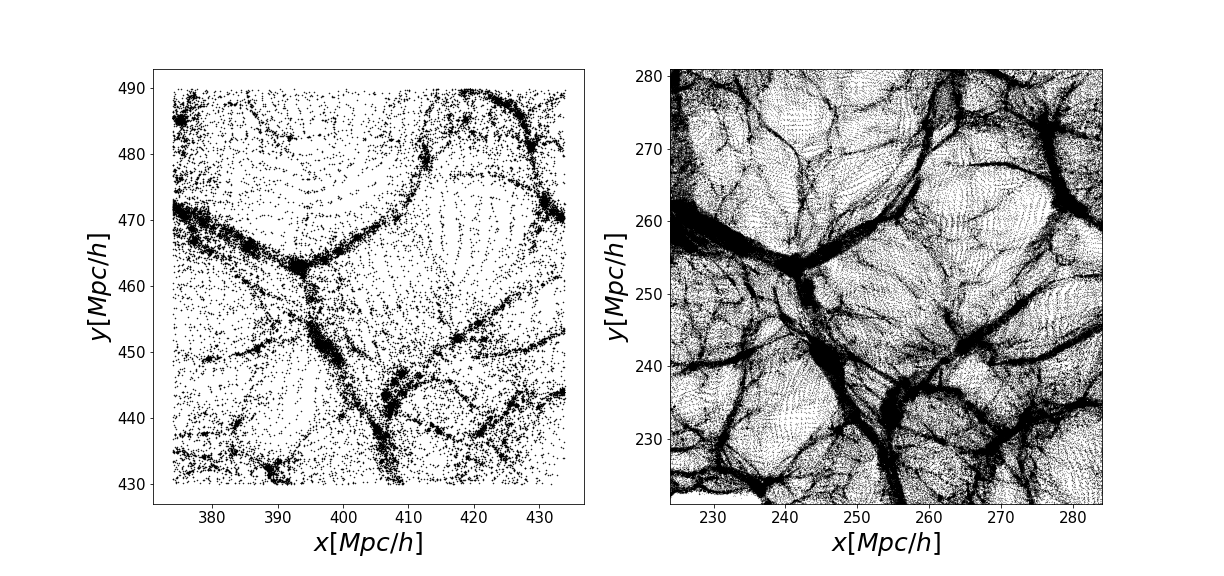
\includegraphics[width=15cm]{Figures/Resi.png}
    \caption{Caption}
    \label{fig:my_label}
\end{figure}{}


En la figura \ref{VoidsIn} se presenta el gas contenido en ambos voids. Ambas secciones pasan por el centro de los voids y la seccion transversal se corresponden al diametro de los voids proyectados sobre el eje z. Los gr\'aficos fueron realizados con el c\'odigo publico \texttt{\textbf{SPH-VIEWER}} \citep{SphViewer}. Este c\'odigo permite estimar los campos de densidad a partir de la implementaci\'on de la t\'ecnica de SPH introduciendo las \textit{longitudes de suavizado} de las particulas. \textbf{PONER ALGO DE ESTO EN LA PARTE SPH CAPITULO}.
\begin{figure}
    \centering
    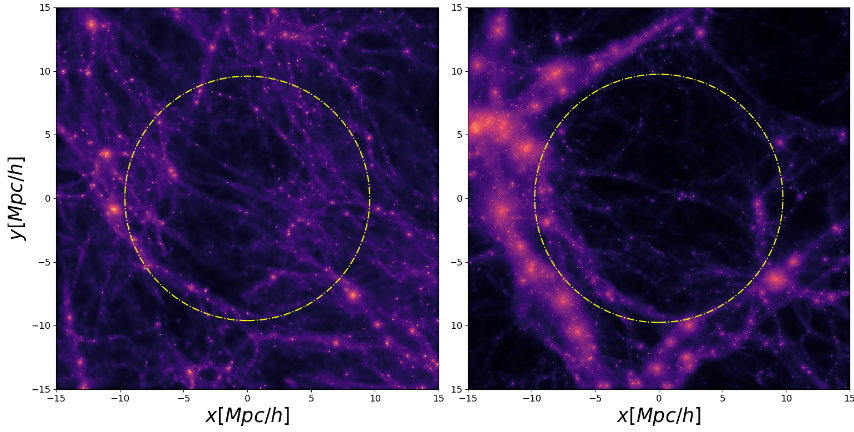
\includegraphics[width=15cm]{Figures/SphVoids.png}
    \caption{Caption}
    \label{VoidsIn}
\end{figure}{}
A partir de \ref{VoidsIn} puede apreciarse como las resimulaciones permiten la obtenci\'on de subestructura dentro de los voids. Podemos ver como estos estan atravezados por una fina red de filamentos y ciertos halos. En el caso del void R, vemos como este carece de una pared sobredensa a diferencia de el void S (derecha) donde vemos como esta envuelto por una gran sobredensidad con importantes nodos. 


\section{Perfiles}




\begin{figure}
    \centering
    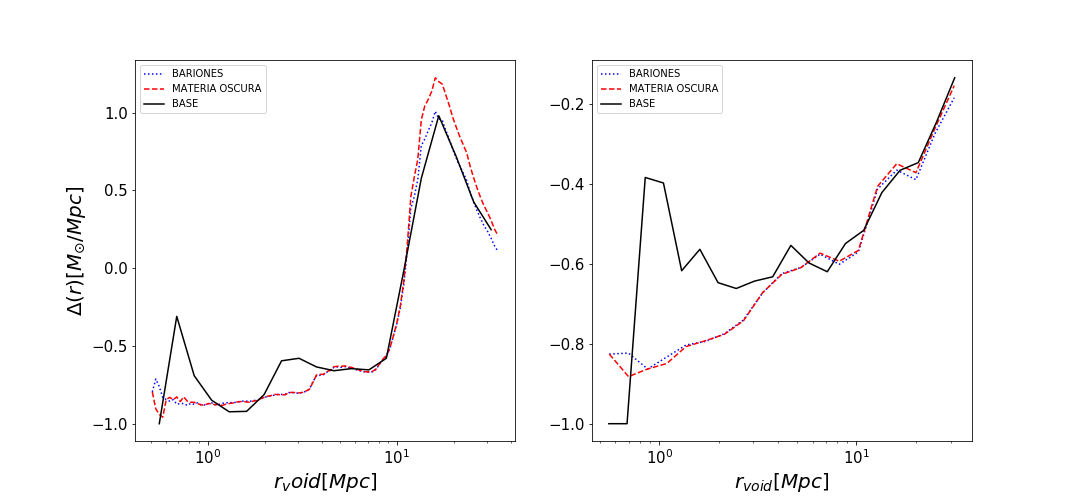
\includegraphics[width=\linewidth]{Figures/PerfilesIntegradsos.png}
    \caption{Caption}
    \label{fig:my_label}
\end{figure}{}

\begin{figure}
    \centering
    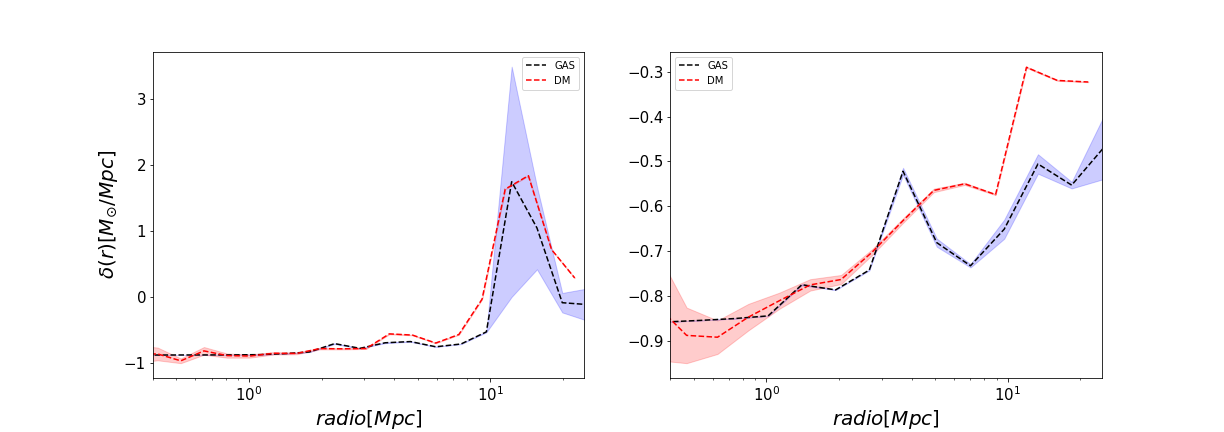
\includegraphics[width=\linewidth]{Figures/perfiles_sph.png}
    \caption{Caption}
    \label{fig:my_label}
\end{figure}{}
\chapter{Propiedades de los halos}
\label{PropiedadesHalos}


En este capitulo nos enfocamos en el an\'alisis de los halos de materia oscura y sus diferentes propiedades bari\'onicas. Tal como se menciono en la seccion ALGUNA las galaxias en los vac\'ios cosmologicos presentan diferentes caracteristicas respecto a aquellas que habitan ambientes de mayor densidad. Es por esto que es esperable que estas diferencias se manifiesten en cuanto a los halos de materia oscura. Con esto en mente, identificamos los halos de materia oscura en los vac\'ios y realizamos una comparaci\'on entre las propiedades de estos dentro de los voids y en las regiones externas. 

\section{Halos y resoluci\'on}

Para la identificaci\'on de halos en las simulaciones, se utiliz\'o el c\'odigo publico \textbf{\texttt{ROCKSTAR}} \citep{Rockstar} (\textit{Robust Overdensity Calculation using K-Space Topologically Adaptive Refinement} ). El c\'odigo se corre solo sobre las particulas de materia oscura de las simulaciones. El \textit{output} del identificador incluye diversas propiedades de los halos encontrados (como la posici\'on del halo, cantidad de particulas o el radio virial $R_{vir}$), pero no es posible conocer \textit{que particulas} pertenecen a cada halo. 

Para conocer que particulas pertenecen a cada halo, uno puede buscar en la simulaci\'on que particulas se encuentran a una cierta distancia del centro del halo (dato otorgado por \textbf{\texttt{ROCKSTAR}}). Siguiendo esta idea se identificaron las particulas que se encuentren a 2 $R_{vir}$ del halo, construyendo asi halos \'esfericos. De esta manera, se estima la poblacion de particulas de gas, estrellas y materia oscura de los halos. Cabe destacar que la forma real de los halos de materia oscura no es esf\'erica (cita ?), raz\'on por la cual se elige buscar part\'icula mas all\'a del $R_{vir}$. 

Debido a que el identificador \textbf{\texttt{ROCKSTAR}} trabaja solo sobre la materia oscura, hay un sesgo en la masa de los halos que construye. El cat\'alogo de halos que se obtiene con el c\'odigo es de estructuras de al menos 10 particulas de materia oscura, pero como vimos en la secci\'on \ref{SPH} las propiedades de las particulas de SPH se distribuyen sobre una regi\'on que alcanza a la n-esima vecina mas cercana. En el caso de \textbf{\texttt{GIZMO}}, n=56 particulas. De modo que para halos de menos de 56 particulas, la 56-vecina de alguna de las particulas SPH del halo va a estar fuera de este, mientras que para un halo de mas de 56 particulas de SPH la 56-vecina de las particulas de gas va a estar dentro del halo. Este razonamiento va en el sentido de decir que las particulas de gas que pertenezcan a un halo que tenga menos de 56 particulas SPH van a tener parte de su masa fuera del halo. De modo que en este trabajo solo se utilizaron aquellos halos que contengan al menos 56 particulas de gas. (EN REALIDAD FUERON 60 ! )

La figura \ref{PlotControl} presenta la relaci\'on de masa de bariones y materia oscura en funci\'on de la cantidad de particulas de los halos. La l\'inea blanca punteada representa a la fracci\'on cosmologica ($\sim 0.18$. Se puede observar que para halos de pocas particulas la relaci\'on $M_{bar}/M_{dm}$ se aleja mucho de el valor te\'orico cosmologico. \textbf{Esto puede deberse a problemas de resoluci\'on?}. La l\'inea amarilla se\~nala 56 particulas, podemos ver que mas all\'a de este valor la fracci\'on $M_{bar}/M_{dm}$ comienza a parecerse a el valor te\'orico. 



\begin{figure}
    \centering
    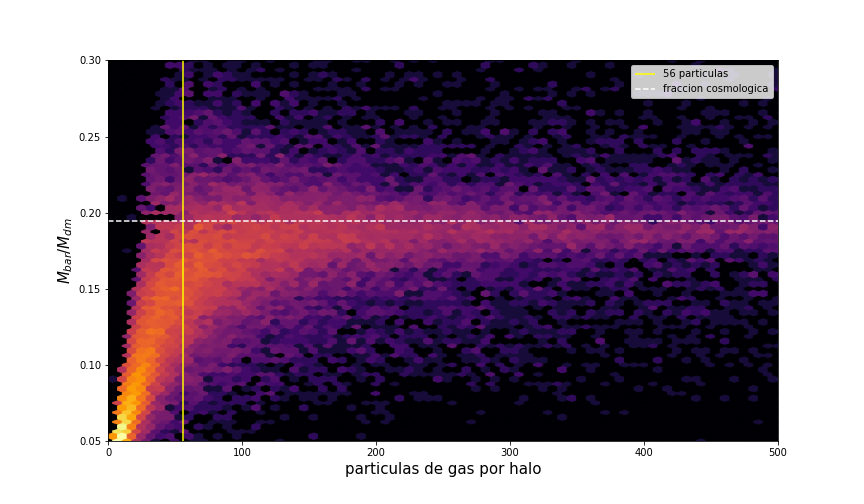
\includegraphics[width=12cm]{Figures/PlotControl.png}
    \caption{Caption}
    \label{PlotControl}
\end{figure}{}


\section{Perfil del Void }

Se explor\'o la posibilidad de que el contenido bari\'onico de los halos de materia oscura tengan alguna dependencia con el entorno, estudiando su distancia al centro del void. Para lo cual se seleccionaron aquellos halos que contengan al menos 56 particulas de gas siguiendo el criterio establecido en la secci\'on anterior y se contruyo el gr\'afico de la figura \ref{PerfilFracciones}.
\begin{figure}
    \centering
    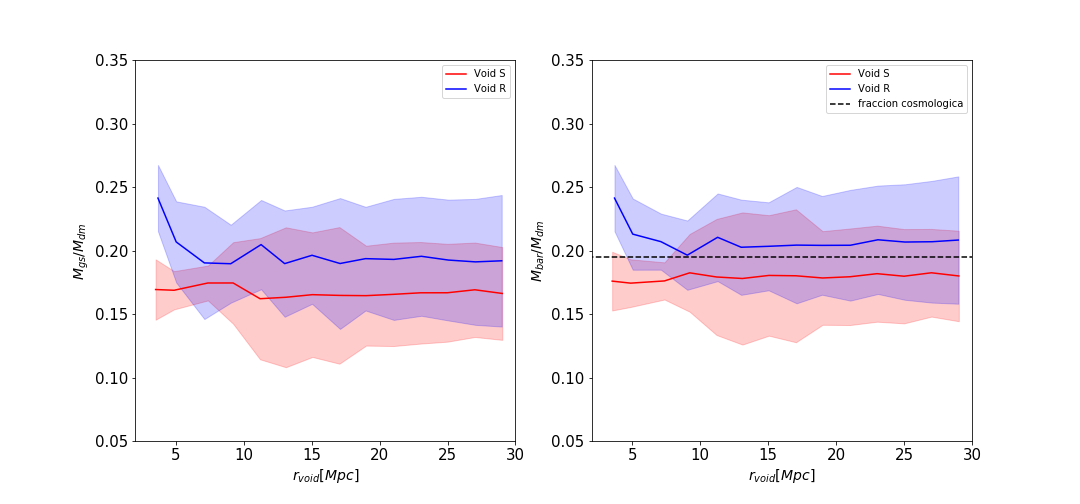
\includegraphics[width=13cm]{Figures/FraccionPerfil.png}
    \caption{Caption}
    \label{PerfilFracciones}
\end{figure}{}
La figura de la izquierda corresponde a la fracci\'on de gas en los halos y la figura de la derecha representa a la fracci\'on de bariones, donde el contenido bari\'onico comprende tanto al gas como las estrellas. Las l\'ineas fueron contruidas teniendo el cuenta la media de cada fracci\'on en cada bin de distancia. La dispersi\'on corresponde a la desviaci\'on est\'andar. 

Si bien la tendencia general es que los halos del void R tengan una fracci\'on mayor de gas o bariones, las diferencias estan contenidas en las dispersi\'ones. En la figura \ref{PerfilFraccionesBar} se presenta la proporsi\'on de estrellas y gas, para halos con al menos una estrella. En este caso la dispersi\'on es demasiado grande y la tendencia no es clara aunque pareciera ser que el void S transformo mas parte de su gas en estrellas, ya que durante la mayor cantidad del perfil tiene una proporsi\'on mayor de estrellas que el void R.  

\begin{figure}
    \centering
    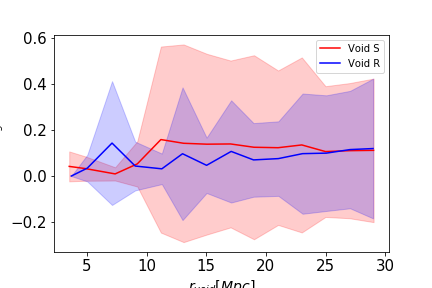
\includegraphics[width=7cm]{Figures/FraccionPerfil_barionic.png}
    \caption{Caption}
    \label{PerfilFraccionesBar}
\end{figure}{}

\section{An\'alisis de regiones}


El prop\'osito de este estudio es identificar que propiedades tienen los halos que pertenezcan a los voids que sean diferentes de las propiedades de halos de entornos mas densos, halos de una regi\'on \textit{homogenea}. Con  esto en mente debemos identificar en nuestras simulaciones alguna regi\'on que pueda ser representativa de un ambiente homog\'eneo. Recurrimos entonces a el contraste de densidad integrado, pero en este caso la integraci\'on se realizara inversamente, es decir, desde \textit{fuera del void} hacia su interior. Definimos entonces:
\begin{equation}
    \Delta_{back}(r)=\int^{in}_{out}\delta(r)dr
\end{equation}{}

Los l\'imites de integraci\'on ser\'an entonces \textit{in}=0 Mpc y \textit{out}=30Mpc. Es importante resaltar que respecto a que hay que tener especial cuidado respecto a el l\'imite externo de integraci\'on (\textit{out}) ya que siempre debemos cuidar de no irnos a regiones tan externas de la simulaci\'on como para contener particulas tidales, ya que como se menciono en la secci\'on ALGUNA estas regiones no estan bien resueltas.

La figura \ref{PerfilesInversos} presenta el contraste de densidad integrado $\Delta_{back}(r)$ desde la regi\'on externa de los voids hacia sus interioriores. De esta manera observamos que en la regi\'on perteneciente a 30-25 Mpc el contraste de densidad es practicamente cero, con lo cual estar\'iamos en una regi\'on \textit{homog\'enea}.

Para seleccionar los halos pertenecientes al void, debemos ir un poco mas all\'a de el radio de cada void. Esto se debe a que la resoluci\'on de las simulaciones realizadas no es suficientemente importante como para obtener una cantidad estad\'isticamente significativa de halos. De modo que debemos relajar un poco el criterio de la definici\'on de void. Clasificamos como halos \textit{del void} aquellos que esten a una distancia tal que $\Delta(r)<-0.7$. Esta condici\'on se cumple a diferentes radios para cada void, siendo entonces $r_{S}=10 Mpc$ y $r_{R}=13 Mpc$.



\begin{figure}[h]
\centering
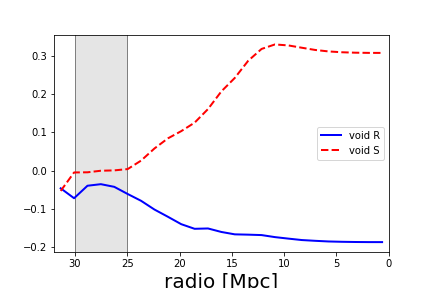
\includegraphics[width=10cm]{Figures/PerfilesInversos.png}
\decoRule
\caption[asd]{}
\label{PerfilesInversos}
\end{figure}

\subsection{Funciones de Masa}




\subsection{Cortes en masa}

Estudiar la dependencia de los halos con el entorno y al mismo tiempo explorar si existe correlaci\'on con la masa de los halos, decidimos separar los halos por bines de masa. De esta manera identificamos los halos realizando 3 cortes indicados en la tabla \ref{CortesMasa}. El criterio para realizar los cortes fue el de mantener significancia estad\'istica. De realizar mas cortes la cantidad de halos en cada uno habr\'ia sido chica como para analizar propiedades globales de las poblaciones.  


\begin{table}[ht]
\begin{tabular}{|l|l|l|l|l|l|}
\hline
  & < 120 particulas  &  120-300 particulas & 300-800 particulas  \\ \hline
S & 48  & 73 &  48              \\ \hline
R & 111  & 92  &    36             \\ \hline
\end{tabular}
\caption{Cantidad de particulas para los halos identificados dentro del void en los diferentes cortes en masa}
\label{CortesMasa}
\end{table}

En la figura \ref{Gs/Dm} presentamos la fracci\'on de masa de gas sobre materia oscura de los halos con los diferentes cortes de masa y diferentes ambientes. Encontramos una tendencia clara en los primeros dos cortes de masa a que los halos de el void S presentan una menor cantidad de gas en relaci\'on a la materia oscura en comparaci\'on al void R. Los halos de fuera de los voids presentan un comportamiento medio entre el de los vac\'ios. Para el tercer corte en masa las distribuciones parecen comportarse similarmente. La l\'inea punteada se\~nala la fracci\'on cosmologica ($\Omega_{bar}/\Omega_{dm}\sim 0.18$). Como en este caso solo estamos mirando las part\'iculas de gas uno podr\'ia pensar que el void S tiene entonces una menor fracci\'on gas/dm debido a que formo estrellas. Para explorar esta idea podemos mirar entonces la fracci\'on bariones sobre materia oscura de los halos.

Las distribuciones de la fracci\'no de bariones sobre materia oscura se presentan en la figura \ref{Bar/Dm} y podemos apreciar que en t\'erminos generales el comportamiento es similar al de la figura \ref{Gs/Dm} donde solo estudiabamos el gas. Esto se debe a que el contenido de estrellas de los halos chicos es insignificante debido a que la resoluci\'on de las simulaciones no alcanza a transformar el gas en estrellas. Con lo cual vemos que los halos de el void S siguen teniendo un menor contenido bari\'onico que los de el R y que los de la regi\'on externa. 

\textbf{MENOS GAS EL VOID S PORQUE TUVO MAS MERGERS. UNA MAYOR TASA DE MERGER VA A HACER QUE EL GAS SE CALIENTE ENTONCES ESTE TENDRA MAYOR TEMPERATURA}


\begin{figure}[h]
\centering
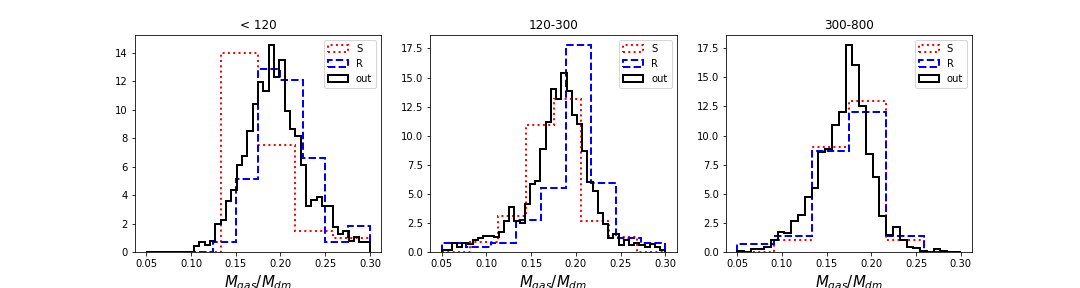
\includegraphics[width=\textwidth]{Figures/Fraccion_cortemasa1.png}
\decoRule
\caption[asd]{Este es fraccion de \textbf{GAS} \textbf{AGREGAR FRACCION COSMOLOGICA}}
\label{Gs/Dm}
\end{figure}


\begin{figure}[h]
\centering
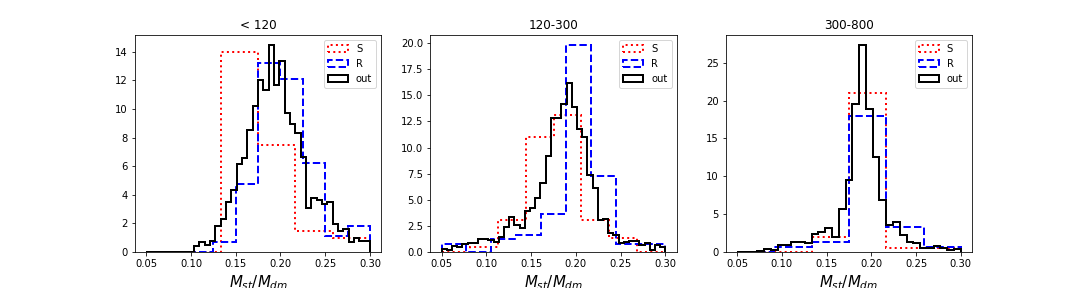
\includegraphics[width=\textwidth]{Figures/Fraccion_cortemasa2.png}
\decoRule
\caption[asd]{Este es fraccion de \textbf{GAS + ESTRELLAS} Entonces las diferencias no se deben a que uno formo mas estrellas que otro. }
\label{Bar/Dm}
\end{figure}


Una propiedad importante para caracterizar el gas es estudiar su temperatura. Podemos asignar una temperatura a un halo considerando el promedio de las temperaturas de gas que lo componen. En la figura \ref{Temperaturas} presentamos la temperatura de los halos. Podemos visualizar una tendencia En las primeras dos regiones (pero fundamentalmente en la primera) a que los halos de el void S estan mas calientes que los halos de el void R, y tambi\'en que los halos de la regi\'on externa. En el tercer corte en masa el comportamiento es contrario ya que la tendencia es que los halos de el void S son mas fr\'ios que los de el R. 


\begin{figure}[h]
\centering
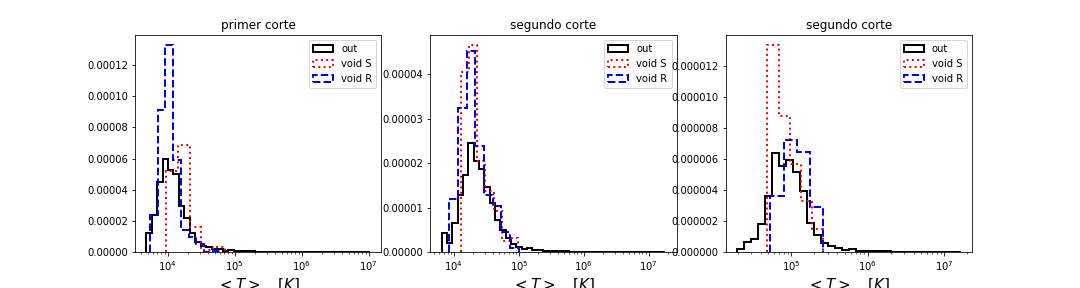
\includegraphics[width=\textwidth]{Figures/temperatura_cortemasa_mean.png}
\decoRule
\caption[asd]{Proba \textbf{sacar el log en el eje y} y meter 11 bines..}
\label{Temperaturas}
\end{figure}

Una posible explicaci\'on para las diferencias encontradas entre el void S y el R en cuanto a la temperatura y contenido de gas de los halos, es que hayan experimentado una tasa de mergers diferentes. Los mergers pueden producir que un halo pierda gas debido a la \textit{ram pressure} \textcolor{red}{\textbf{BUSCAR CITA CLASES HERNAN}} y al mismo tiempo el gas que conserve el halo aumente su temperatura. Debido a que la din\'amica de los voids S y R es fundamentalmente diferente ya que unos se hayan en expansi\'on y otros en contracci\'on, es esperable que la historia de mergers de sus halos sea diferente. \textcolor{green}{Recordemos que las diferencias observadas corresponden a los primeros dos cortes en masa. Mergers de halos grandes son poco probables, lo mas esperable es que los halos grandes \textit{mergen} con halos chicos, pero halos pequen\~os afectaran en menor medida las propiedades de el halo grande, en comparaci\'on a el \textit{merger} de dos halos pequen\~os, y esta podr\'ia ser la raz\'on por la cual no vemos muchas diferencias entre las propiedades de los halos en el tercer corte en masa.}


En la figura \ref{DensCorteMasa} se indica las densidades de gas y materia oscura de los halos $(\rho_{gs}$ y $\rho_{dm}$. Esta densidad es la masa que contiene el halo dividido el radio del mismo (recordemos que los identificamos como 2 $R_{vir}$. Si observamos la densidad de gas, podemos observar una tendencia marginal de los halos del void S a ser mas densos que los halos del void R. Los halos fuera del void pueden alcanzar densidades tanto menores como mayores pero esto se debe a que la muestra es significativamente mayor. No se percibe una tendencia sistem\'atica a un comportamiento caracter\'istico de estos. Al observar la densidad de materia oscura, una comparaci\'on entre los voids para indicar de nuevo que los halos del void S son mas densos que los del R, con la misma salvedad indicada para los halos fuera del void. 






\begin{figure}[h]
\centering
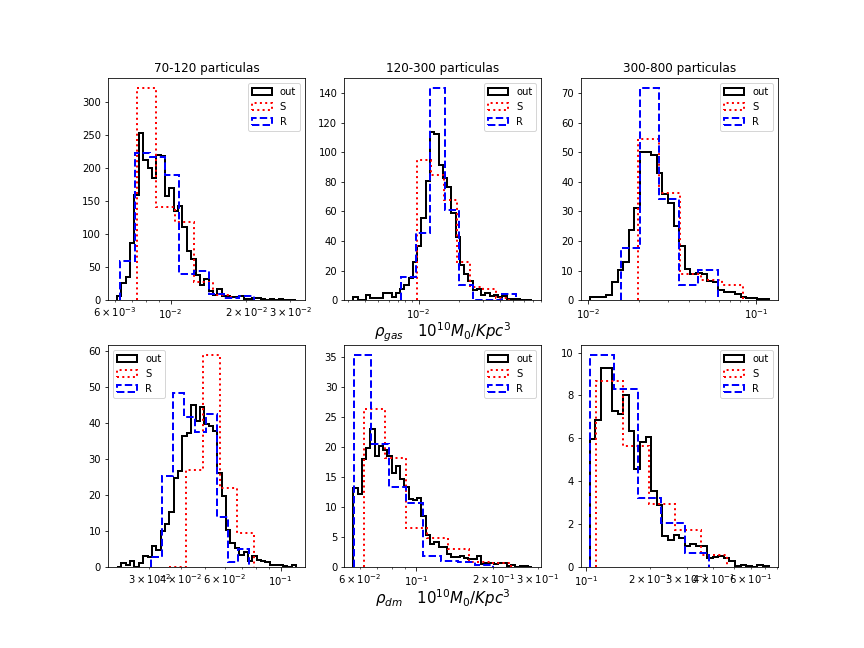
\includegraphics[width=\textwidth]{Figures/Densidades_cortemasa.png}
\decoRule
\caption[asd]{Esta densidad es la cantidad de particulas del halo en 2 radios viriales dividido esta distancia. }
\label{DensCorteMasa}
\end{figure}

Si bien la se\~nal encontrada en la figura \ref{DensCorteMasa} es muy d\'ebil, parecer\'ia indicar que los halos de el void S son m\'as densos que los de el void R, y esto es compatible con lo sen\~alado respecto a que puedade deberse a una diferente historia de \textit{mergers}.



%\begin{figure}[h]
%\centering
%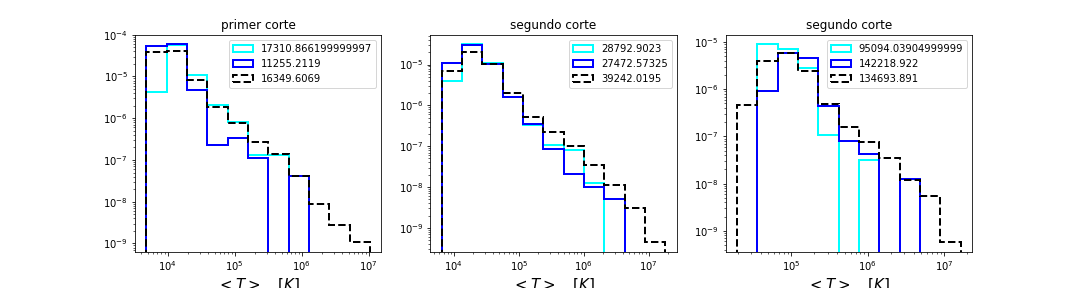
\includegraphics[width=10cm]{Figures/temperatura_cortemasa_median.png}
%\decoRule
%\caption[asd]{}
%\label{fig:Electron}
%\end{figure}


%Para el primer corte
%\begin{tabular}{c|c|c|c|c}
%    - & media & $\sigma/\sqrt{n}$ & mediana & rango cuadratico \\
% \hline   S & 47482.2 & 12608 & 17310& 9036\\
% \hline   R & 47675.3 & 16175 & 11255 & 5170\\
%\hline    U & 166890.1 & 17029  & 16349 &35189.\\

%\hline
%\end{tabular}{}

%Para el segundo corte
%\begin{tabular}{c|c|c|c|c}
%    - & media & $\sigma/\sqrt{n}$ & mediana & rango cuadratico \\
% \hline   S & 96689& 25194 & 28792 & 9036\\
% \hline   R & 89407 & 29988 & 27472 & 5170\\
%\hline    U & 359823 & 26899 & 39242 & 92987\\
%
%\hline
%\end{tabular}{}


%\begin{table}[]
%\begin{tabular}{|l|l|l|l|l|l|}
%\hline
%  & mean                          & $\sigma/\sqrt{n}$ & median & iqs & 92987 \\ \hline
%S & 4.7 $10^{4}$ & 1.3 $10^{4}$            & 0.05   &     &       \\ \hline
%R & 4.7 $10^{4}$ & 1.6 $10^{4}$             & 0.07   &     &       \\ \hline
%U & 1.7 $10^{5}$ & 1.7 $10^{4}$               & 0.06   &     &       \\ \hline
%\end{tabular}
%\end{table}

\section{Entornos Locales}

Un enfoque complementario a lo desarrollado hasta aqu\'i es estudiar el entorno de las estrellas, independientemente de las propiedades de los halos. Si bien todas las estrellas forman parte de halos conceptualmente estamos haciendo algo diferente. 

Estudiaremos entonces el entorno local de las estrellas observando las densidades de materia oscura, gas y estrellas mismas. De esta manera buscamos cuantificar si la formaci\'on estelar en las regiones subdensas presenta caracter\'isticas particulares en comparaci\'on de la contraparte de una mayor densidad. 
 Para realizar esto medimos la distancia a la n-\'esima vecina y utilizamos esta distancia para contruir densidades locales. 

Teniendo en cuenta que tenemos casi 10 veces mas particulas de gas o materia oscura que particulas de estrellas, estimamos las densidades locales utilizando la distancia a la 50-vecina mas cercana para el gas y la materia oscura ($\rho_{gs}$ y $\rho_{dm}$) y la 5-vecina mas cercana para las estrellas ( $\rho_{st}$). Los resultados se presentan en la figura \ref{densidades locales}. Se presentan entonces la densidad de estrellas, gas y materia oscura alrededor de las particulas estelares en nuestra simulaci\'on. 

A la izquierda en la figura \ref{densidades locales} se presenta el entorno estelar. No apreciamos diferencias significativas entre los voids y afuera de estos, aunque pareciera existir una leve se\~nal de que el void R presenta una mayor densidad estelar aunque lejos de ser significativa. 

\begin{figure}
    \centering
    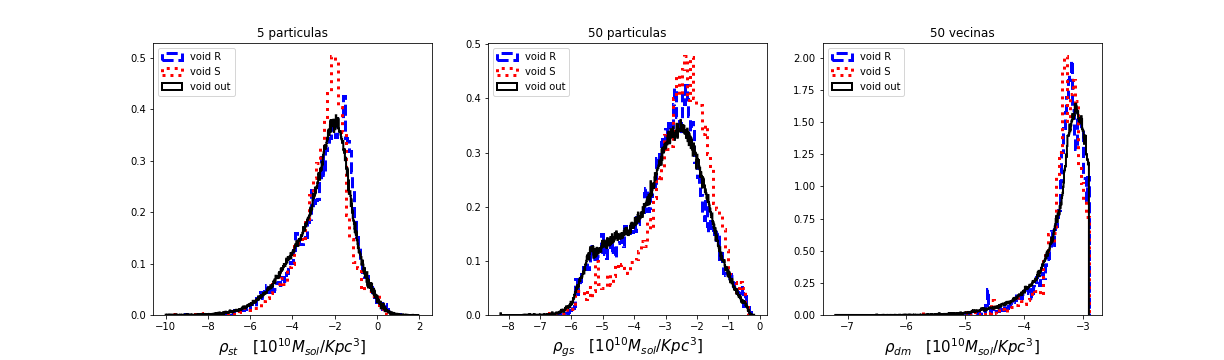
\includegraphics[width=\textwidth]{Figures/densidades_locales.png}
    \caption{Caption}
    \label{densidades locales}
\end{figure}{}

La densidad de gas se presenta en la figura central. Se tiene aqui que el void R y la regi\'on externa se comportan practicamente igual. El caso del void S es mas interesante porque pareciera existir una tendencia a ser mas denso en gas. 

Para estudiar la materia oscura se realiz\'o un corte para eliminar aquellas particulas que presenten una densidad mucho mas all\'a de la longitud de \textit{softening} ($l_{s}$) de la simulaci\'on, ya que a estas escalas tenemos muchas impresiciones en cuanto a la integraci\'on de las particulas. De modo que el corte se realiz\'o en lo que corresponde a una densidad local estimada en un radio de $\sim 1.8 l_{s}$. Tenemos entonces el resultado a la derecha de la figura \ref{densidades locales} donde se observa una leve tendencia en los voids a ser menos densos que la regi\'on externa. Particularmente el void S siendo menos denso que el R. 


El estudio del entorno local aqu\'i representado no es del todo robusto ya que se cuantifica la densidad utilizando una cantidad fija de particulas vecinas y esto no permite estimar la densidad en mas de una escala. Un estudio mas adecuado ser\'ia llevado al cabo utilizando funciones de correlaci\'on, pudiendo de esta manera cuantificar la densidad en una ampl\'ia gama de escalas. 

A\'un bajo estas limitaciones, se observo una tendencia de el void S a tener una mayor densidad de gas alrededor de sus estrellas, lo cual cuadra con lo se\~nalado en la secci\'on anterior ya que como se observo los halos del void S tenian una mayor temperatura. Si el gas se encuentra cercano a las estrellas el \textit{feedback} de estas lo calentara. 

\section{Resumen}
Arranque viendo que los halos del S tiene un mayor contenido de estrellas pesados por masa de gas. Al mismo tiempo en el S tengo menos gas/dm que en el R. Esto lo veo en las fracciones en funcion de los perfiles pero tambien en los primeros dos cortes en masa. Teniendo en cuenta que estan mas calientes y que la densidad de gas alrededor de estrellas es mayor puede deberse a que el feedback calienta el gas y por eos estan mas calientes. Por otro lado, una mayor tasa de mergers pudo por un lado desencadenar procesos de formaci\'on estelar y por otro lado haberle arrancado parte del gas, siendo por esto que tienen menos gas/dm y mas st/gs. (\textbf{aunque el menor st/gs puede ser simplemente porque tiene menos gas...}
\chapter{Estudio de Diagramas de Fases}
\label{DF}





\section{Diagrama de Fases}
\begin{figure}
    \centering
    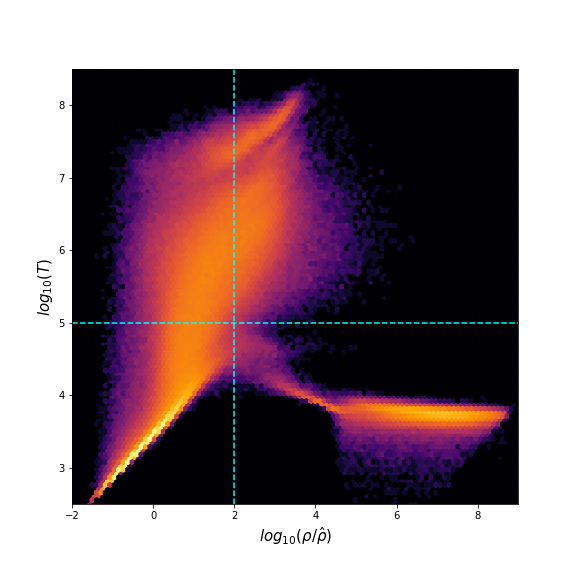
\includegraphics[width=14cm]{Figures/DF.png}
    \caption{Diagrama de Fase de la simulacion cosmologica. $\hat{\rho}$ es la desnidad media barionica del universo. NO HAY PROBLEMA CON LA FRACCION DE ESTRELLAS? Aca estoy alcanzando densidades de 8, que son altas (generalmente solo alcanzan hasta 6, ej paper que nos paso fede) pero debe ser por el modelo de SF, ya que aca da igual \citep{Springel2002}. KE ONDA. Poner etiqueta de las regiones}
    \label{DF}
\end{figure}{}

Las propiedades de los bariones pueden ser estudiadas observando los diagramas de fases, como el de la figura \ref{DF} donde las particulas de SPH se binean en el espacio de densidad y temperatura. Los procesos astrof\'isicos que ocurren a medida que el universo va evolucionando producen que las particulas de gas experimenten cambios en su densidad y temperatura. El colapso de los halos producen aumentos de densidad en el gas, feedback de supernovas producen aumento de la temperatura del gas, etc. 

Debido entonces a procesos astrof\'isicos, el gas va atravesando diferentes regiones del diagrama de fases, delimitadas por densidad y temperatura (linea punteada figura \ref{DF}. Estas regiones representan a particulas de gas que comparten ciertas propiedades f\'isicas en t\'erminos generales. Diversos autores utilizan diferentes criterios para clasificar de esta manera al gas (\cite{Schaal2016}, \cite{Martizzi2019}). En este trabajo se adopta el criterio utilizado por \citep{Huang2019} debido a que su simplicidad permite captar de manera general el comportamiento del gas. 

De esta manera entonces el gas se encuentra en el universo en 4 fases divididas por una temperatura  de  T=$10^{5}$K y una densidad $\delta_{th}$ definida por \citep{Kitayama1996} (( \citet{Dave2010} ACA ESTA BIEN, EN EL DE FEDE ESTA MAL LA FORMULA !!)) aquella en la que los halos se encuentran virilizados FIJATE BIEN ESTO:

\begin{equation}
    \delta_ {th}=6\pi^{2}(1+0.4093(1/f_{\Omega}-1)^{0.9052}-1
\end{equation}{}

\begin{equation}
    f_{\Omega}=\frac{\Omega_{m}(1+z)^{3}}{\Omega_{m}(1+z)^{3} + (1-\Omega_ {m} - \Omega_{\Lambda})(1+z)^{2} + \Omega_{\Lambda}}
\end{equation}{}
\begin{itemize}
    \item Gas difuso: Este gas es primordial, de baja densidad. La mayoria de este se encuentra en una curva que establece un balance entre enfriamiento adiab\'atico y calentamiento por fotoionizaci\'on. 
    \item WHIM: Las particulas de gas de esta regi\'on se encuentras ionizadas y a bajas densidades ya que son desplazadas aqu\'i debido a que en su proceso de colapso a los halos son calentadas por \textit{shocks} y frenan su caida a los halos.
    \item Condensado: Esta fase contiene gas frio que se encuentra dentro de los halos. 
    \item Caliente: Este gas se encuentra dentro de los halos, \textit{shocks} y \textit{feedbacks} debido a procesos astrof\'isicos elevan su temperatura. 
\end{itemize}{}
Cabe destacar que una quinta regi\'on se debe a el gas con formaci\'on estelar. Es gas dentro de los halos (condensado). Pero la resoluci\'on obtenida en nuestras simulaciones hace que en general las particulas pasen de estar Condensadas a convertirse en estrellas, sin permanecer mucho tiempo en la region de formaci\'on estelar. Es debido a esto que decidimos omitir esta regi\'on en el an\'alisis siguiente. 





\section{Perfiles del gas}

Tal como se sen\~alo con anterioridad, el gas en el universo se encuentra en diferentes \textit{fases} segun sus caracteristicas f\'isicas y sus propiedades f\'isicas van a depender de el entorno en el que se encuentren. De modo que las diferentes fases del gas trazan diferentemente las estructuras del universo, en particulas los perfiles de los vac\'ios cosmol\'ogicos. 

La tabla \ref{FraccionesGasTabla} contiene las fracciones $(f_{fase})$ de las fases en las que se encuentra el universo actual. Con esta informaci\'on es posible conocer la densidad media de cada fase $\hat{\rho}_{fase}$ que va a venir dada por:
\begin{equation}
    \hat{\rho}_{fase}=\rho_{crit}\Omega_{bar}f_{fase}
\end{equation}{}

Conociendo la densidad media de las fases es posible calcular el contraste de densidad siguiendo la ecuaci\'on \ref{ContrasteDensidad} y de esta manera podemos construir los perfiles de la figura \ref{PerfilGas}.


\begin{figure}
    \centering
    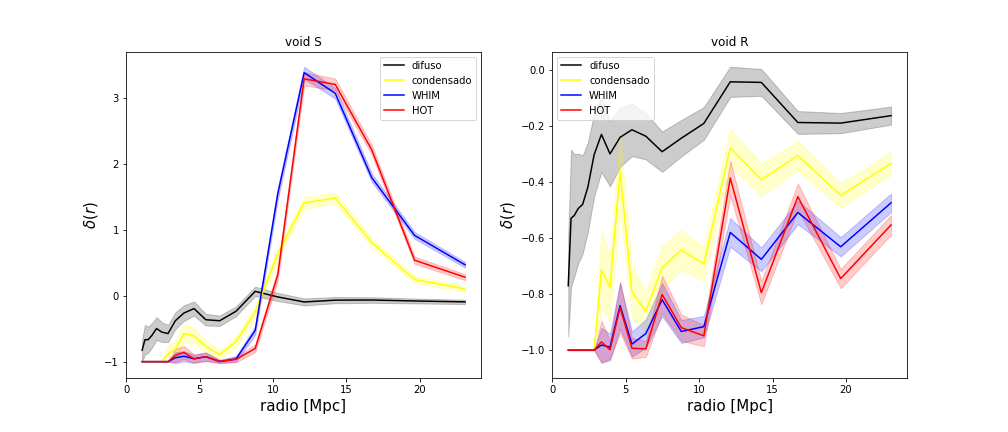
\includegraphics[width=14cm]{Figures/perfilgas.png}
    \caption{Caption}
    \label{PerfilGas}
\end{figure}{}

Es interesante observar que las diferentes fases del gas trazan la estructura de manera muy diferente. En el caso de el void S podemos ver como el gas \textit{Whim} y \textit{HOT} trazan la pared de el vac\'io de una manera muy pronunciada, mientras que el gas \textit{condensado} es sensible a la pared pero de forma menos intensa. El gas \textit{difuso} parece ser impermeable a la estructura ya que casi no presenta variaciones a lo largo del perfil, solo en el centro del void dentro de $\sim 5$ Mpc se observa un decrecimiento significativo de este perfil. 

El perfil de el void R presenta un crecimiento continuo desde el centro del vac\'io hacia el exterior. En el caso de el gas difuso el comportamiento parece ser similar a el void S ya que tenemos que crece fuertemente hasta $\sim 5$ Mpc pero luego parece estabilizarse, mas all\'a de un leve pico en el radio del void ($r\sim10$ Mpc. Las dem\'as fases de el gas trazan el perfil de una manera similar marcando un continu\'o crecimiento. 

Una diferencia importante parece ser marcada por el gas condensado y el gas caliente (en sus dos fases \textit{HOT} y \textit{WHIM}). Para el void S el gas condensado tiene un contraste menos intenso, mientras que para el void R el gas condensado tiene un contraste siempre mayor que el gas caliente. \textcolor{green}{Esto podr\'ia deberse a que el void S tiene una pared muy importante de gran densidad, donde se concentran los procesos de formaci\'on estelar, que mediante el feedback se encargan de calentar el gas y marcando de esta manera el contraste de densidad intenso que se observa para el gas en sus fases caliente.}

En la figura \ref{VoidFases} observamos un corte transversal que pasa por el centro del void S donde podemos ver donde se encuentra el gas de cada Fase. Podemos ver que el contraste es mas t\'enue en el gas difuso, que lo podemos encontrar tanto en las estructuras filamentosas que se observan como en la regi\'on interna que pertenece al centro del void. El gas \textit{condensado} y \textit{hot} se encuentra en regiones localizadas de los filamentos, en los halos. Esto es obvio ya que estamos hablando de gas a alta densidad que se encuentra colapsado en los halos de materia oscura. El gas \textit{WHIM} se encuentra como podemos ver en la estructura filamentosa que circunda al void. Esta gas es calentado en el proceso de colapso de los halos por lo cual es esperable que se halle entonces cerca de los mismos. 

\begin{figure}
    \centering
    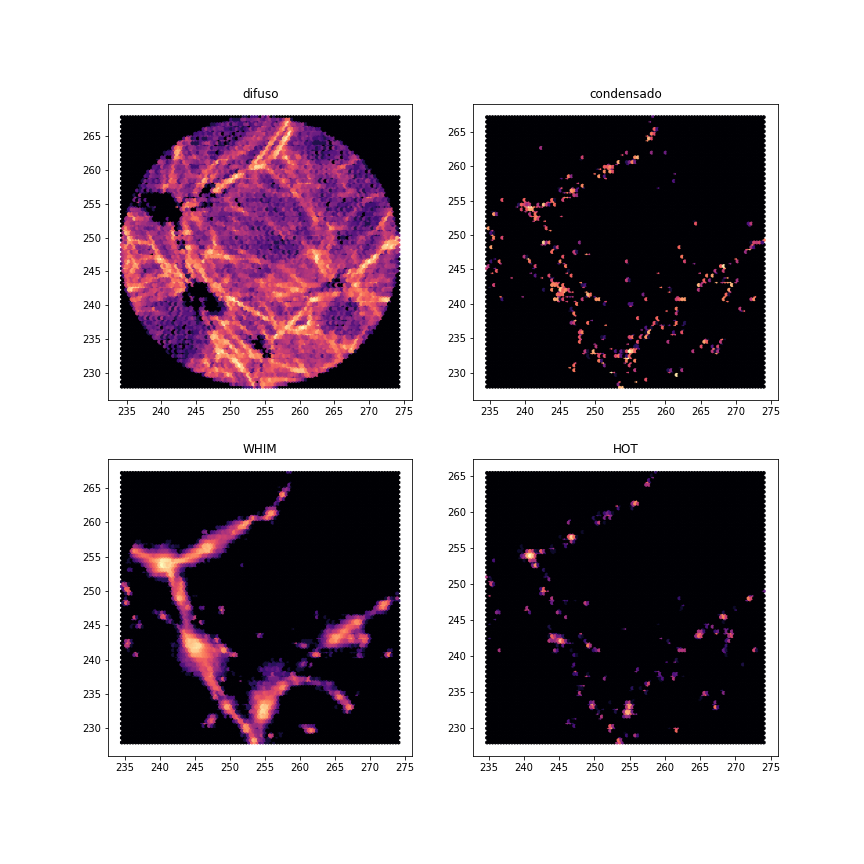
\includegraphics[width=14cm]{Figures/FasesHexbin_S.png}
    \caption{Caption}
    \label{VoidFases}
\end{figure}{}

\section{Universos pristinos}

Galaxias que habitan los voids tienen una historia de formaci\'on estelar y evoluci\'on qu\'mica de aquellas que habitan entornos de mas alta densidad. REF  (see e.g. Peebles 2001;Gottl ̈ober et al. 2003; Hoeft et al. 2006; Hahn et al. 2007a,b, andreferences therein).

Esto puede entenderse ya que los voids poseen un flujo de halos hacia las paredes de los mismos. (ACA MANDAR A EL PLOT DE EL PERF DE VELOCIDADES) por lo que la historia evolutiva de los halos y sus mergers va a ser diferente de aquellos halos que habiten entornos de mas alta densidad. En particular es esperable que la tasa de mergers de galaxias sea menor en los voids, de esta manera, las galaxias que habiten estos entornos ser\'an menos evolucionadas. 

Estas propiedades observadas de las galaxias que habitan los voids \citep{Kreckel2016} permiten pensar a los voids como universos pristinos, en el sentido de que las galaxias que habiten estos ambientes podr\'ian ser representativas de la poblaci\'on de galaxias de un universo temprano a alto redshift. 

Con motivo de explorar esta idea nos centramos en el estudio de los diagramas de fases, para evaluar en que medida las fracciones de bariones en cada fase del gas dentro de los voids puede compararse con las fracciones de bariones de el universo temprano. Es esperable que el universo temprano presente un mayor contenido de gas \textit{difuso} y menor contenido de gas dentro de los halos, ya sea en su fase de \textit{condensado} o \textit{caliente}. La figura \ref{TimeMachine} (central) presenta en diagrama de fases del universo a $z\sim3.2$ donde efectivamente podemos observar lo se\~nalado. La mayor parte del gas ocupa la region correspondiente a gas \textit{difuso} (un $\sim 85\%$) en comparaci\'on de al universo a z=0 donde el gas difuso ocupa un $\sim45\%$


\begin{table}[ht]
\begin{tabular}{c|c|c|c|c|c}
    - & void S & void R & universo $z\sim 3.2$ &universo $z\sim 2.7$ &universo z=0 \\
\hline    difuso     & 86.2  & 81.1  & 87.1  &  82.6   & 44.7\\
\hline    WHIM       & 1.6   & 4.2   & 2.2   &  4.2    & 24.8\\
\hline    caliente   & 2.3   & 4.5   & 1.1   &  2.3    & 16.8\\
\hline    condensado & 9.8   & 10.1  & 9.4   &  10.9   & 14.3\\
\hline
\end{tabular}
\caption{..}
\label{FraccionesGasTabla}
\end{table}

De modo que puede realizarse una comparaci\'on \textit{gruesa} estudiando fracciones de bariones dentro del void a z=0 con una regi\'on homogenea del universo a diferentes redshifts para ver donde son mas similares las fracciones de gas. Para lo cual se utilizo la simulacion BASE ?? Externo al vOIDS?? 

Para seleccionar las particulas pertenecientes al void, se busco que el contraste adimencional de densidad integrado de la masa sea $\Delta(r)_{masa}<-0.6$. Esto se corresponde a los radios $r_{S}=8.1Mpc$ y $r_{R}=8.8 Mpc$ para los diferentes voids. Con las particulas seleccionadas dentro de estos radios se contruyeron los diagramas de fase de la figura \ref{TimeMachine} (izquierda y derecha). 


La figura \ref{Error} representa el error cuadr\'atico (\ref{ErrorFormula}) de las fracciones de gas del void-universo a diferentes edades. Podemos observar que el universo a $z\sim2.9$ se asemeja al void R, mientras que a $z\sim3.5$ el se asemeja al void S, en este \'ultimo caso, las similitudes son mayores. 


\begin{equation}
    \epsilon=\sum_{i=fases}(f^{void}_{i}-f^{univ}_{i})^{2}
    \label{ErrorFormula}
\end{equation}{}


Una primera vista a la figura \ref{TimeMachine} permite apreciar la similitud de los diagramas de fases. Practicamente observamos una carencia de particulas calientes a diferencia de el diagrama \ref{DF}. Esto se debe, en el caso del universo a z$\sim$3 a que los halos no han terminado de colapsarse y los que hay son peque\~nos. Esto produce que no hayan formado una cantidad suficiente de estrellas como para calentar el entorno. En el caso de los voids, al ser ambientes subdensos el proceso de formaci\'on de los halos se retrasa respecto a el universo en general. De esta manera es que se traza una similitud entre los voids y su similitud con el universo pristino. 

\textbf{Llama la atenci\'on que nuestra epoca de myor similitud coincide con la epoca de mayor formaci\'on estelear de nuestras simulaciones.}





\begin{figure}
    \centering
    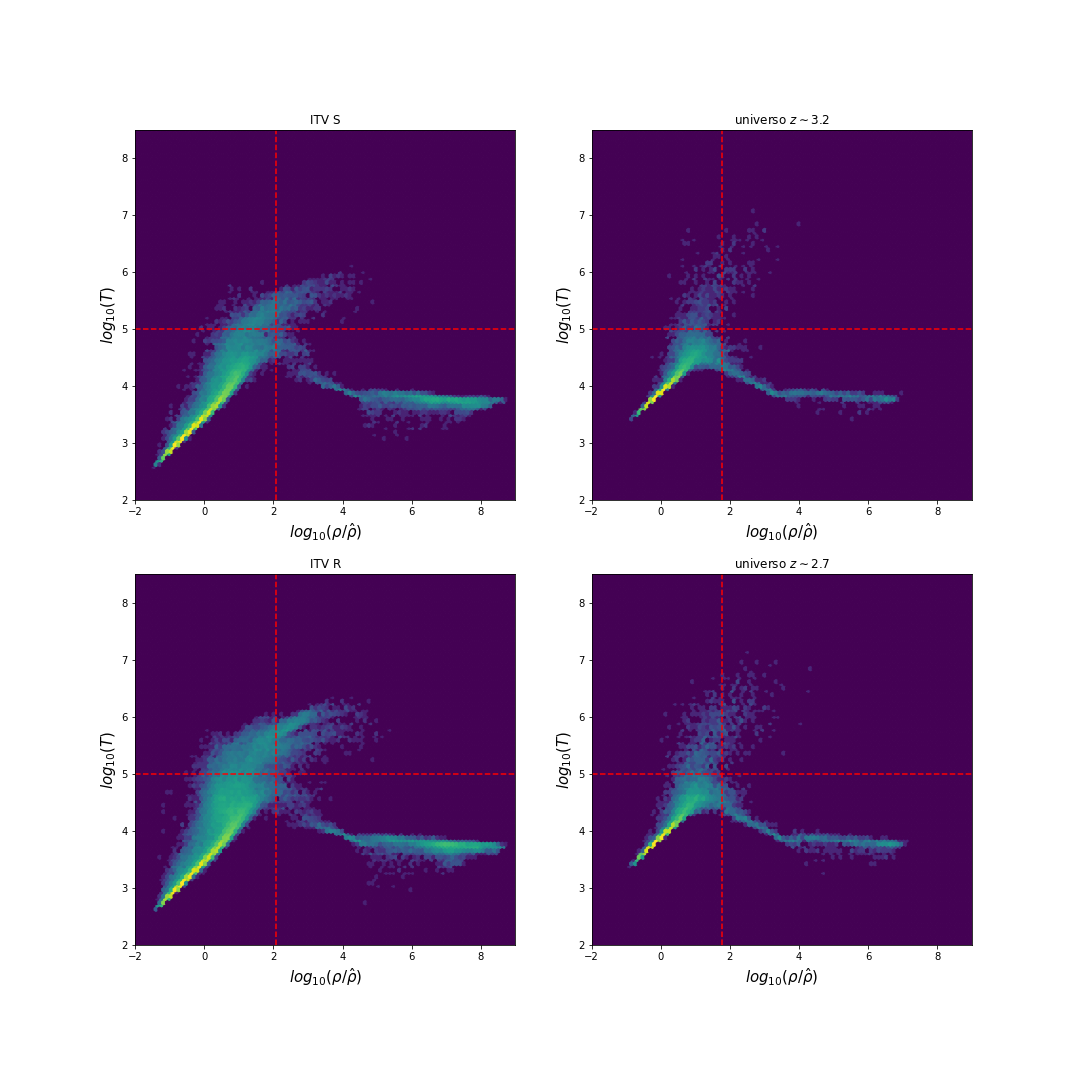
\includegraphics[width=14cm]{Figures/TimeMachine_DF.png}
    \caption{Caption}
    \label{TimeMachine}
\end{figure}{}

\begin{figure}
    \centering
    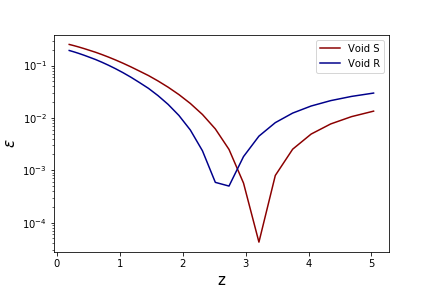
\includegraphics[width=12cm]{Figures/TimeMachine_error.png}
    \caption{Error cuadratico de las fracciones de gas del universo en comparaci\'on a los voids. }
    \label{Error}
\end{figure}{}

Como puede apreciarse en la figura \ref{TimeMachine} el gas difuso parece comportarse como una relaci\'on de potencia entre la densidad y la temperatura. Esto fue estudiado por \citep{Hui1997} donde se demostro que existe una relaci\'on de tal naturaleza que modela los procesos de contracci\'on adiab\'atica y calentamiento por fotoionizaci\'on. 
\begin{equation}
    T=T_{0}(1+\delta)^{\gamma-1}
    \label{EcuacionEstado}
\end{equation}{}
La relaci\'on \ref{EcuacionEstado} modela entonces el comportamiento del gas poco denso del IGM. 







\chapter{Simulaciones utilizadas} % Main appendix title

\label{Apendice} % For referencing this appendix elsewhere, use \ref{AppendixA}

\begin{table}[ht]
\begin{tabular}{c|c|c|c|c|c}
    - & n_{dm} & n_{gs}  &  m_{dm}   & m_{gs}   & box [Mpc] \\
\hline    Base     & 500^{3}  & -  & &  &  500   \\
\hline    Void S   & 3.0 10^{7}   &  3.0 10^{7} & 9.3 10^{8} &1.8 10^{8} & 80    \\
\hline    Void R   & 3.6 10^{7}   & 3.6 10^{7}   &9.3 10^{8} & 1.8 10^{8} & 80  \\
\hline    Ref      & 9.8   & 10.1  & 9.3 10^{8}    &1.8 10^{8} & 120 \\
\hline
\end{tabular}
\caption{..}
\label{Simulaciones0}
\end{table}

\begin{figure}
    \centering
    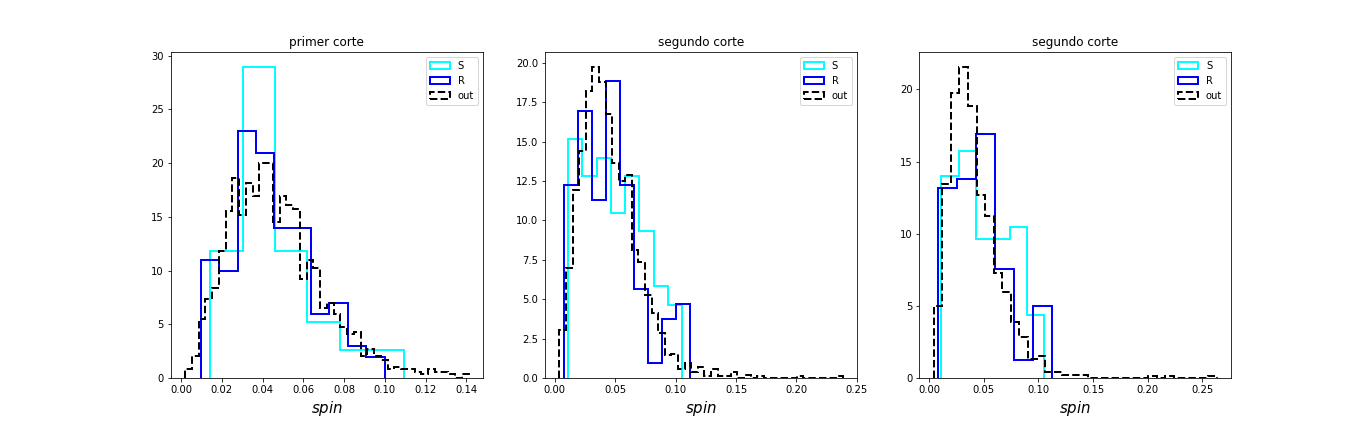
\includegraphics[width=13cm]{Figures/Spin_cortemasa.png}
    \caption{Caption}
    \label{fig:my_label}
\end{figure}{}
%% Chapter 1

\chapter{GAS/DM} % Main chapter title

\label{Chapter1} % For referencing the chapter elsewhere, use \ref{Chapter1} 

%----------------------------------------------------------------------------------------

% Define some commands to keep the formatting separated from the content 
\newcommand{\keyword}[1]{\textbf{#1}}
\newcommand{\tabhead}[1]{\textbf{#1}}
\newcommand{\code}[1]{\texttt{#1}}
\newcommand{\file}[1]{\texttt{\bfseries#1}}
\newcommand{\option}[1]{\texttt{\itshape#1}}

%----------------------------------------------------------------------------------------

\section{}









\section{Figures}


\begin{figure}[h]
\centering
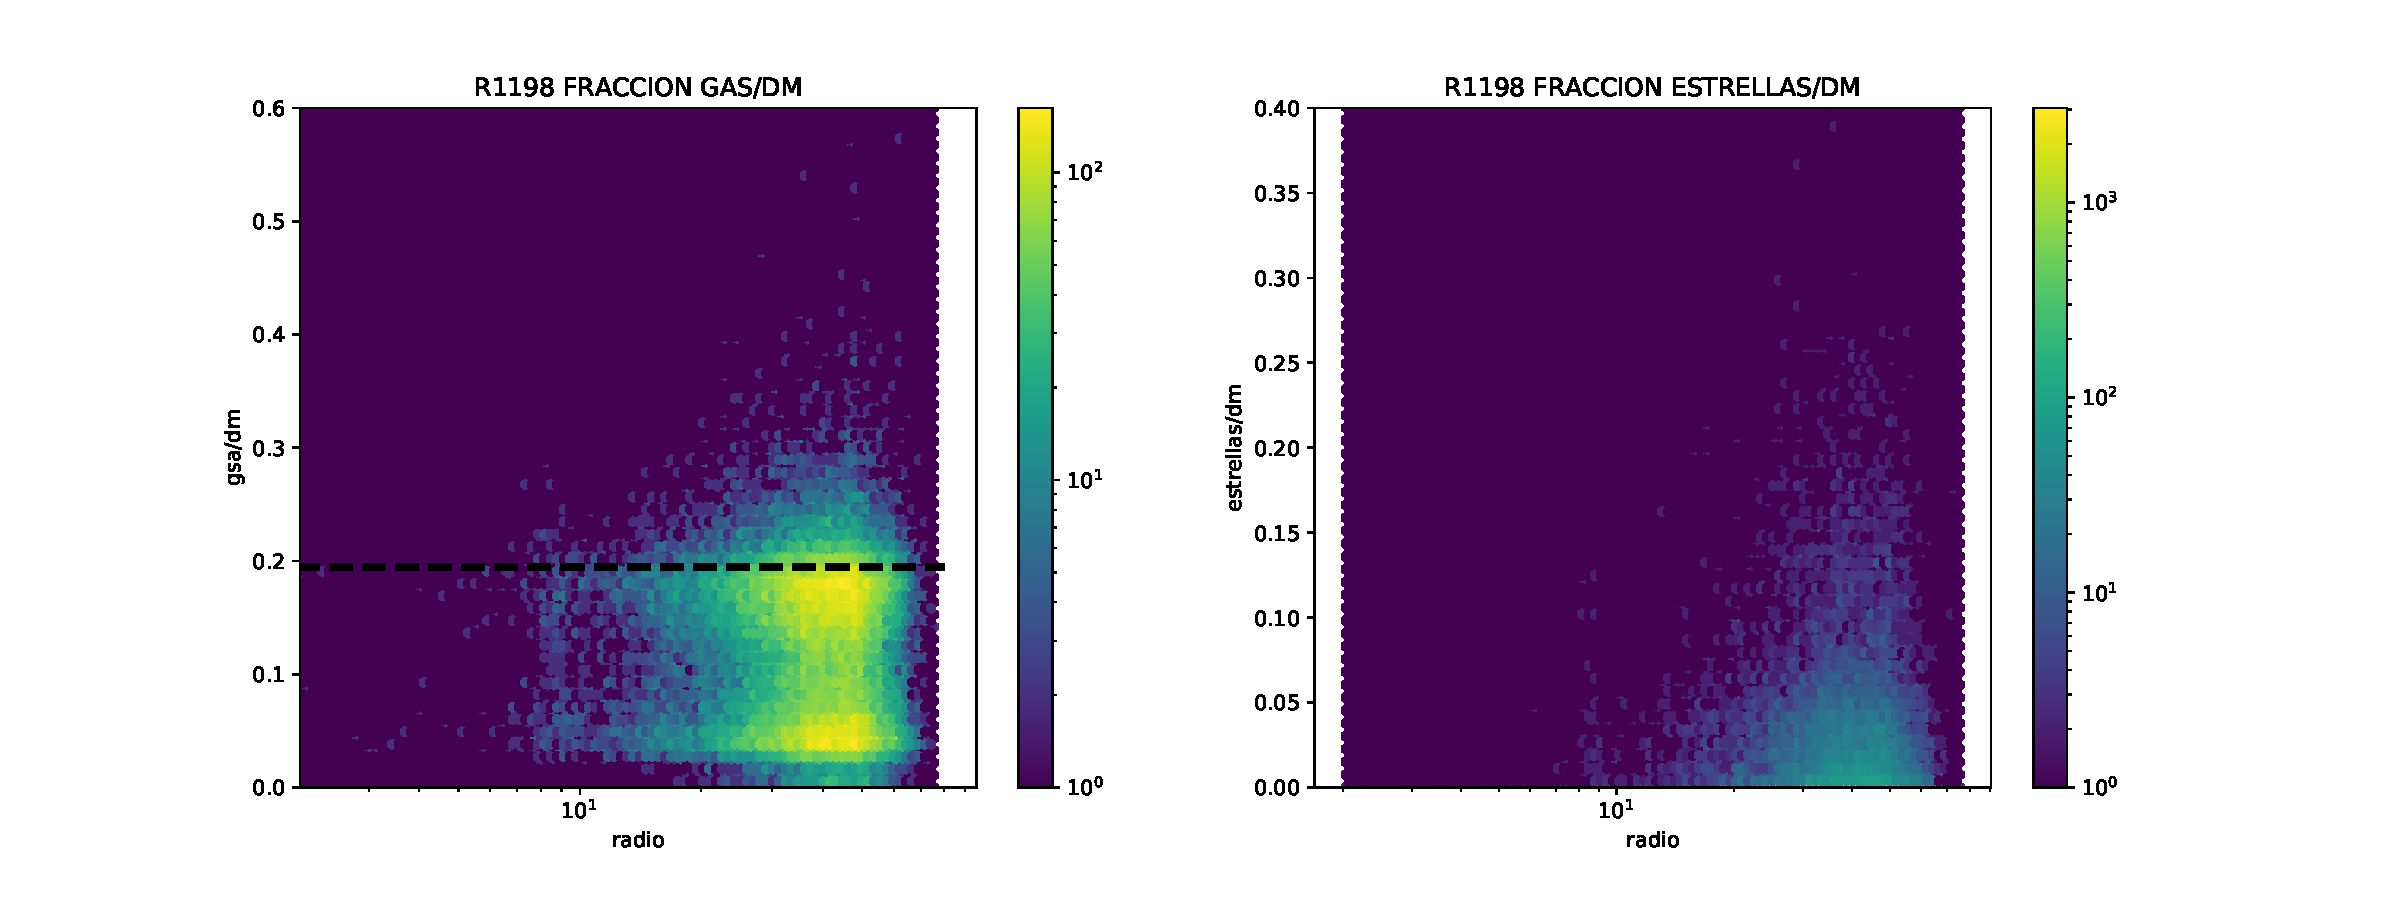
\includegraphics[width=1\textwidth]{Figures/R1198_scatterFRACCIONES.pdf}
\decoRule
\caption[R1198 BARIONES/DM perfil (scatter) ]{Fraccion de gas sobre DM en funcion del centro del void, tamaño del void $\sim$ 9.5 Mpc. A la derecha la fraccion es de Estrellas sobre DM}
\label{fig:Electron}
\end{figure}

\begin{figure}[h]
\centering
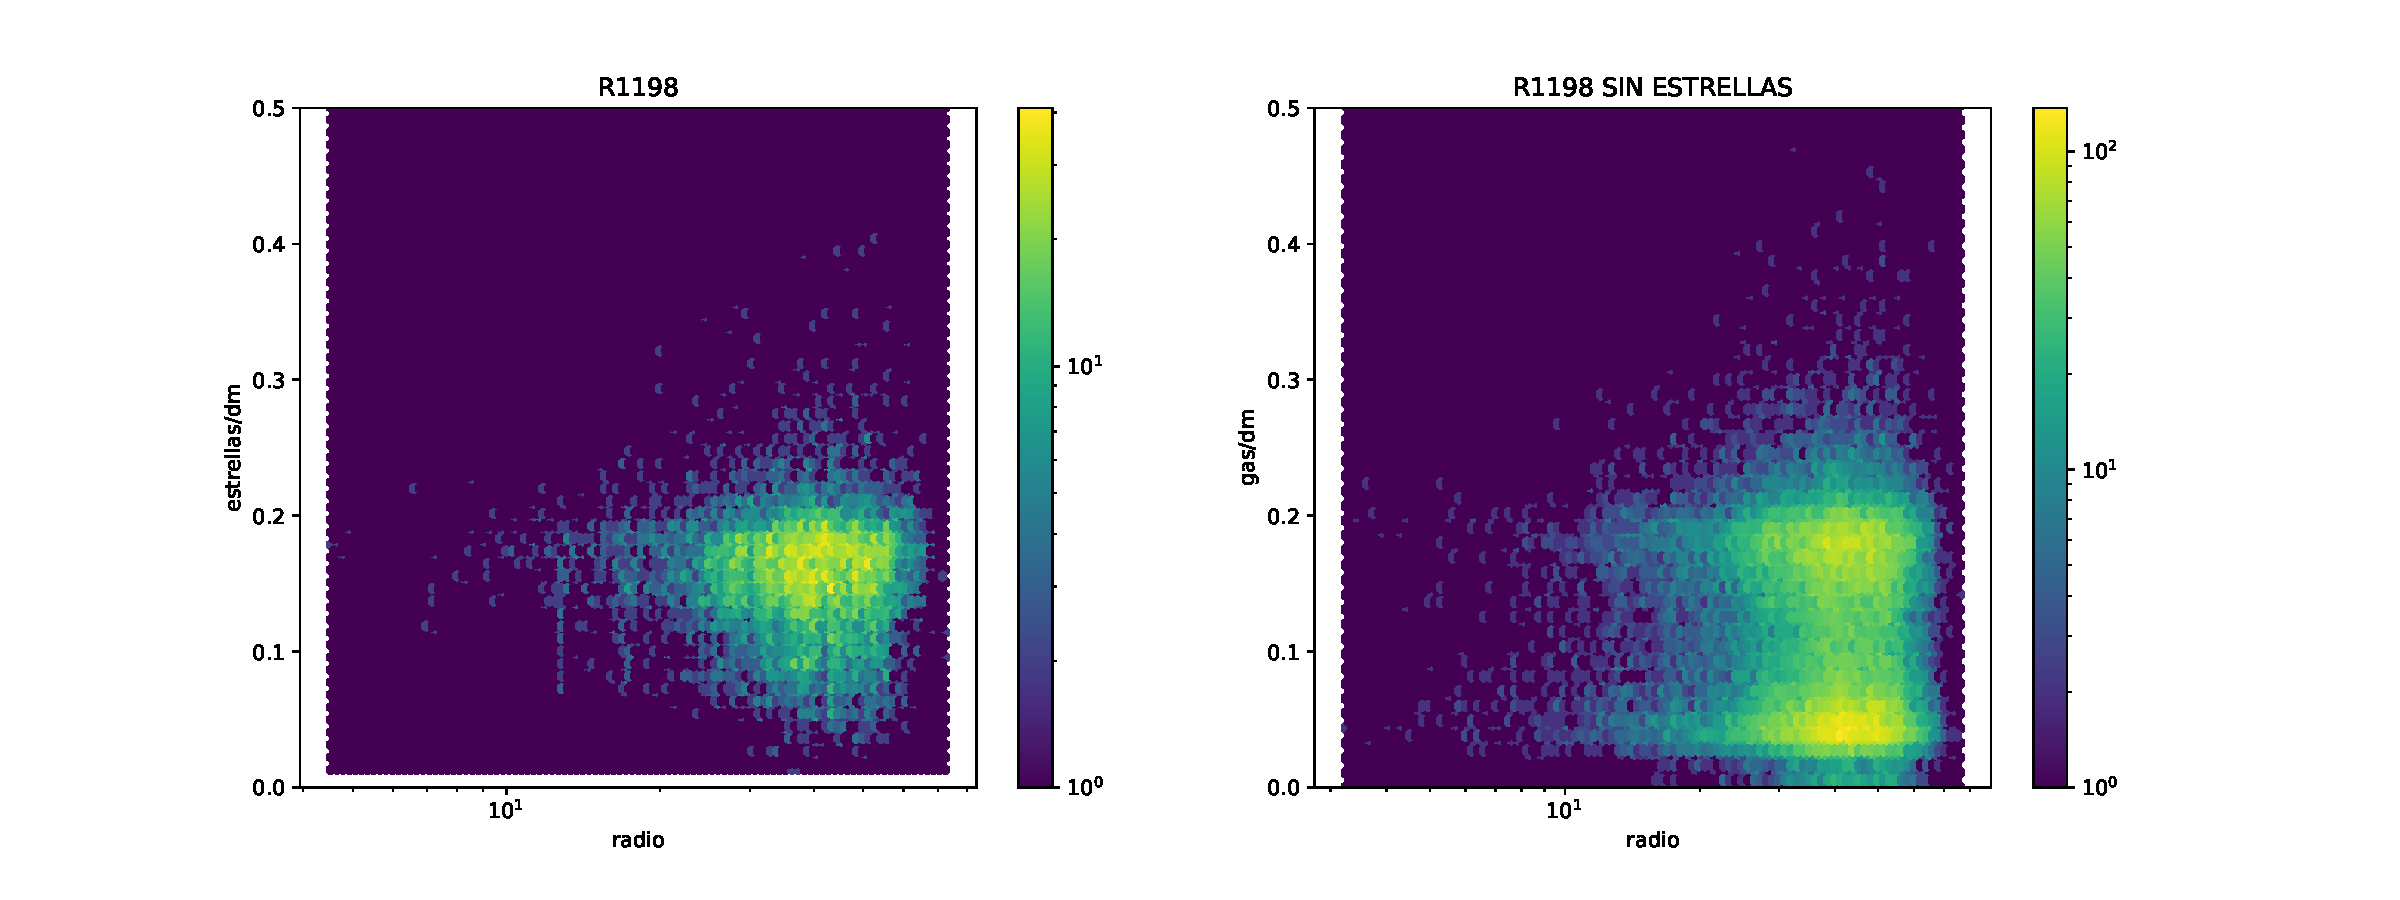
\includegraphics[width=1\textwidth]{Figures/R1198_scatterFRACCIONES_con&sinEST.pdf}
\decoRule
\caption[R1198 GAS/DM perfil (scatter) con y sin estrells]{Perfil de gas/dm para los halos. A  la izquierda estan los halos que contienen al menos una particula de estrellas. A la derehc a los que no tienen ninguna estrella}
\label{fig:Electron}
\end{figure}

\begin{figure}[h]
\centering
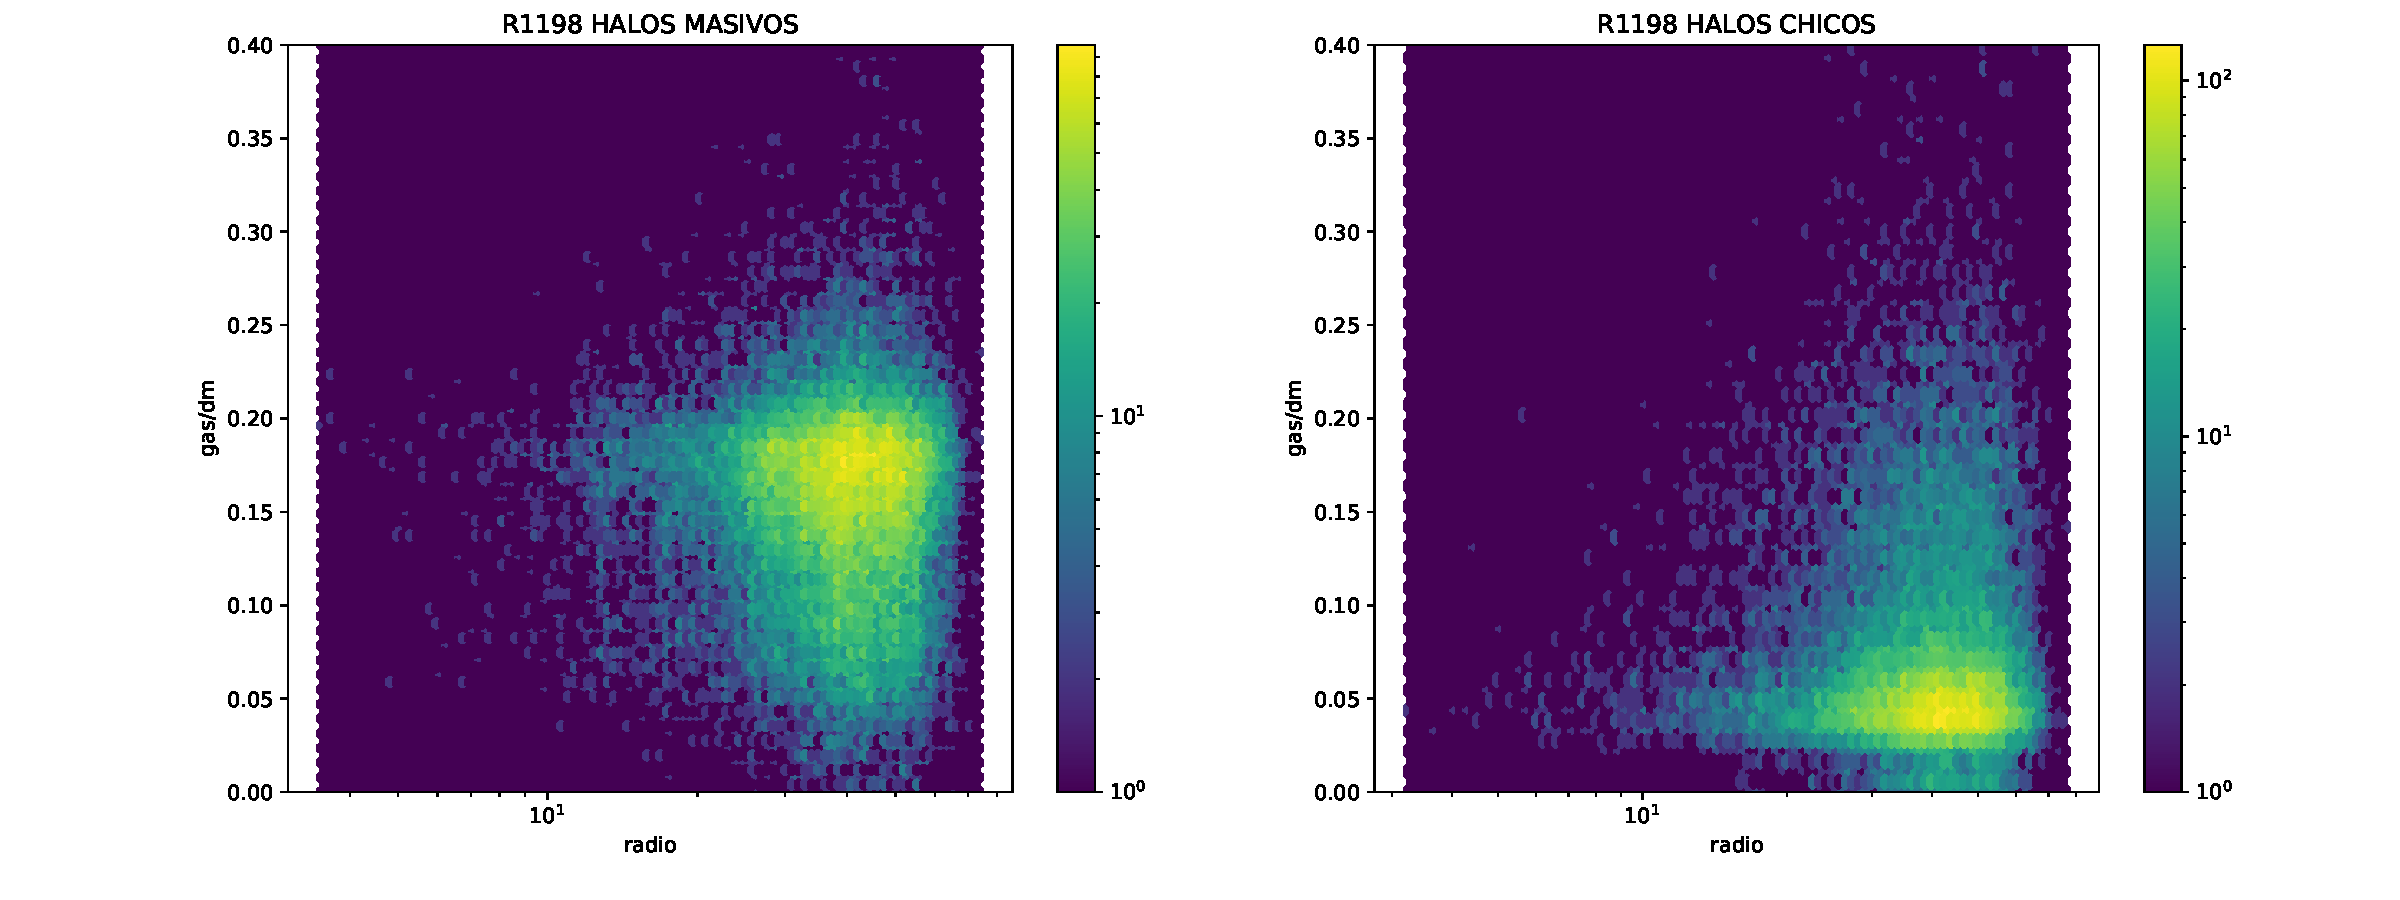
\includegraphics[width=1\textwidth]{Figures/R1198_scatterFRACCIONES_grandesYchicos.pdf}
\decoRule
\caption[R1198 GAS/DM perfil (scatter) halos grandes y chisos]{fraccion de gas sobre DM separando los halos por tamaño. Los halos GRANDES tienen mas de 50 particulas de DM, los chicos menos de 50. }
\label{fig:Electron}
\end{figure}


\begin{figure}[h]
\centering
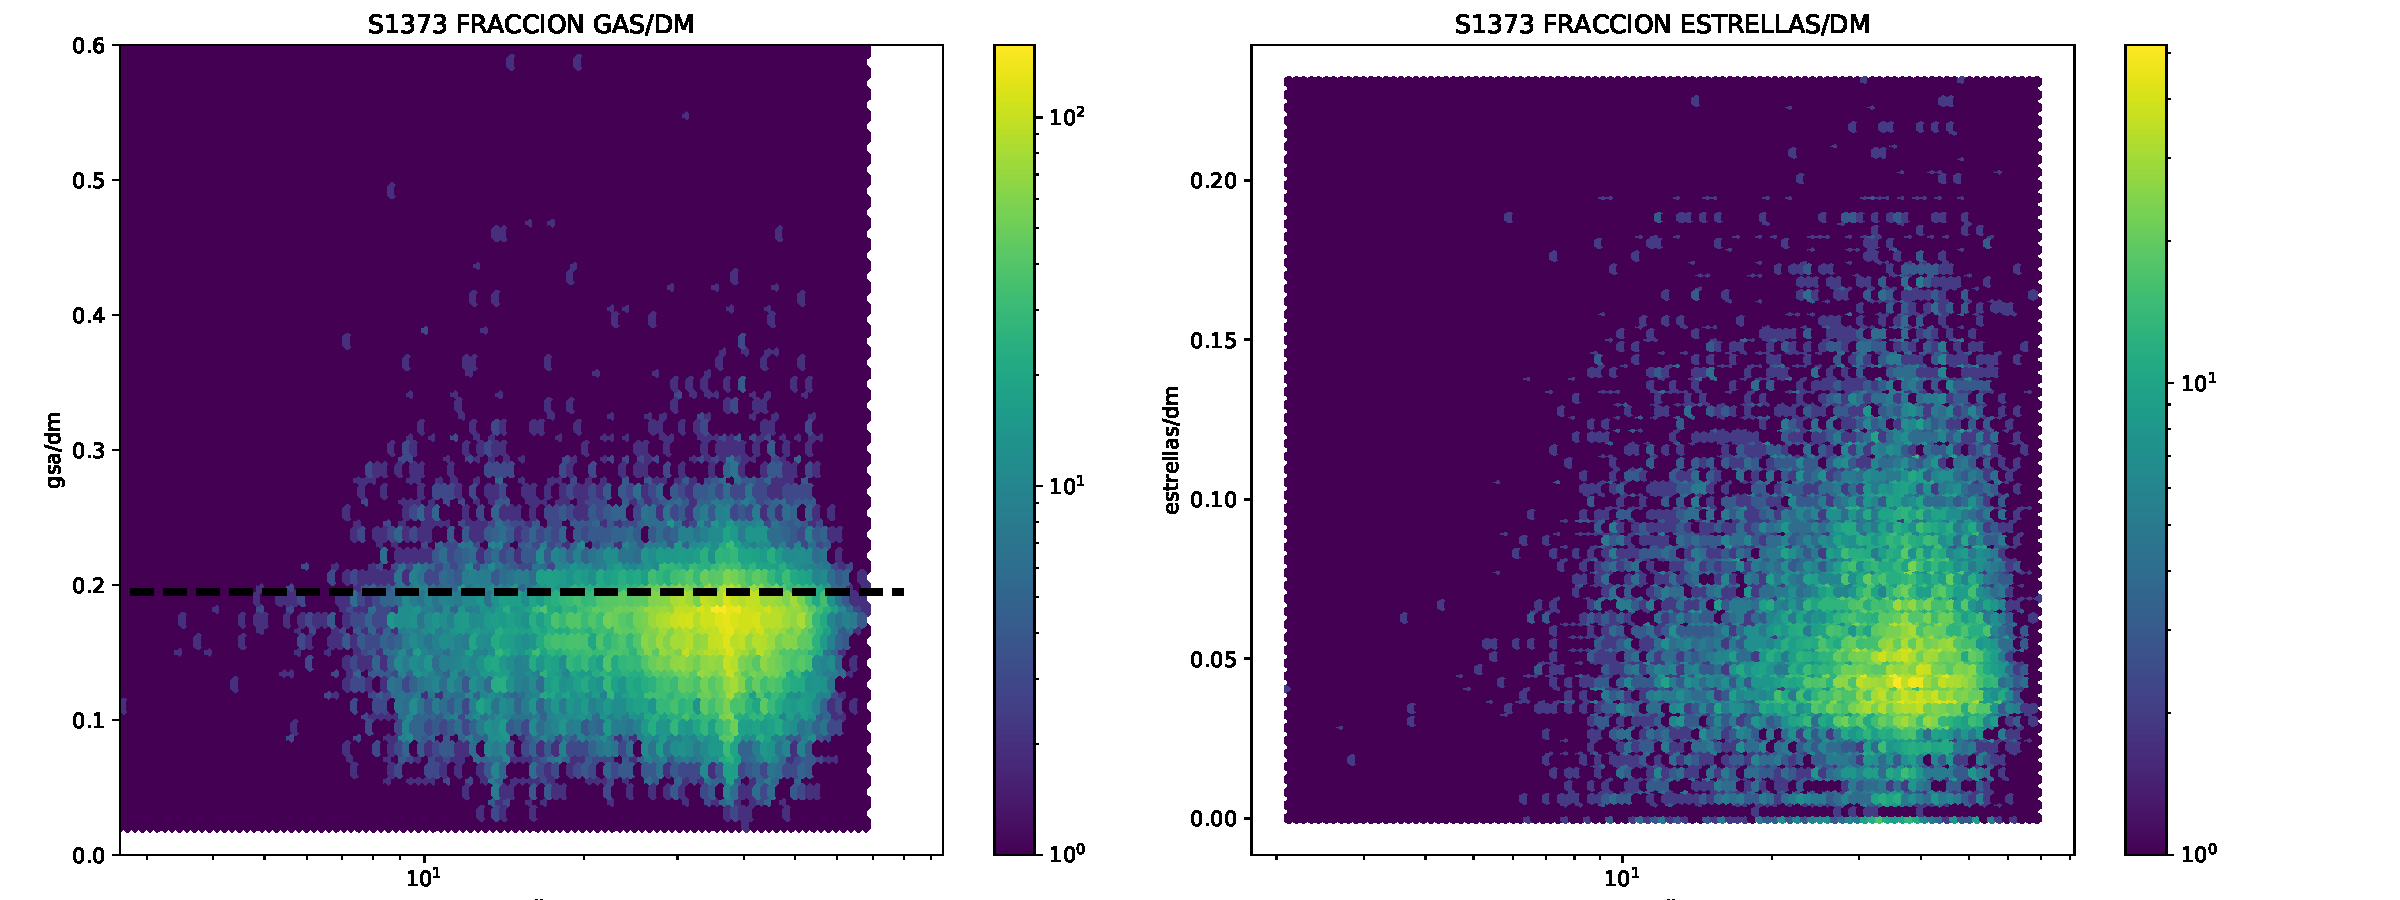
\includegraphics[width=18cm]{Figures/S1373_scatterFRACCIONES2.pdf}
\decoRule
\caption[S1373 GAS/DM perfil (scatter)]{El SPH considera las 32 ? particulas mas cercanas para calcular el hsml, entonces un halo que tenga al menos 32 particulas de gas va a tener sus 23 vecinas en el halo (casi seguro) entonces la masa de gas de ese halo van a ser todas las particulas en el (IZQUIERDA). A unn halos con menos de 32 particulas de gas, le va a pasar que sus particulas de gas van a tener masa FUERA del halo DERECHA).}
\label{fig:Electron}
\end{figure}








\begin{figure}[h]
\centering
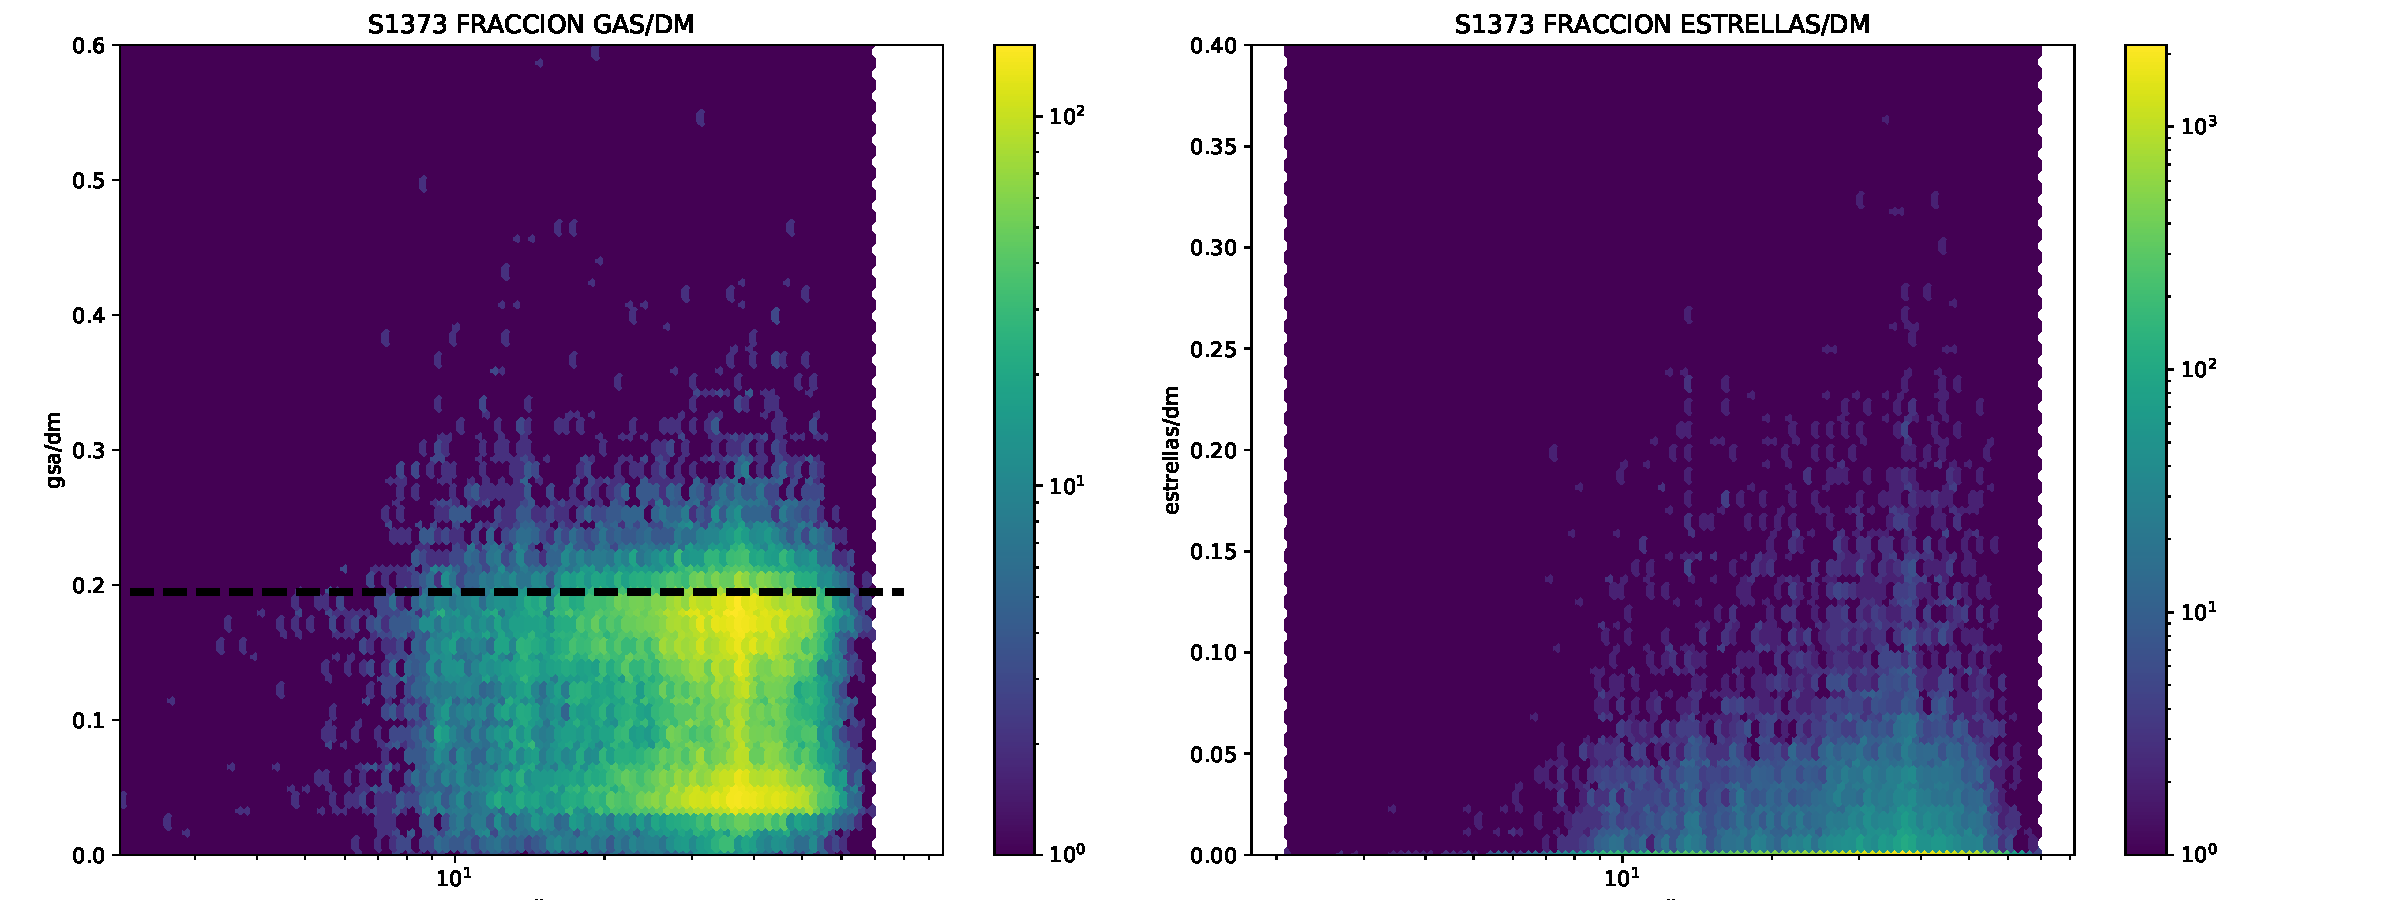
\includegraphics[width=18cm]{Figures/S1373_scatterFRACCIONES.pdf}
\decoRule
\caption[S1373 GAS/DM perfil (scatter)]{Fraccion de gas sobre DM en funcion del centro del void, tamaño del void $\sim$ 9.5 Mpc. A la derecha la fraccion es de Estrellas sobre DM}
\label{fig:Electron}
\end{figure}

\begin{figure}[h]
\centering
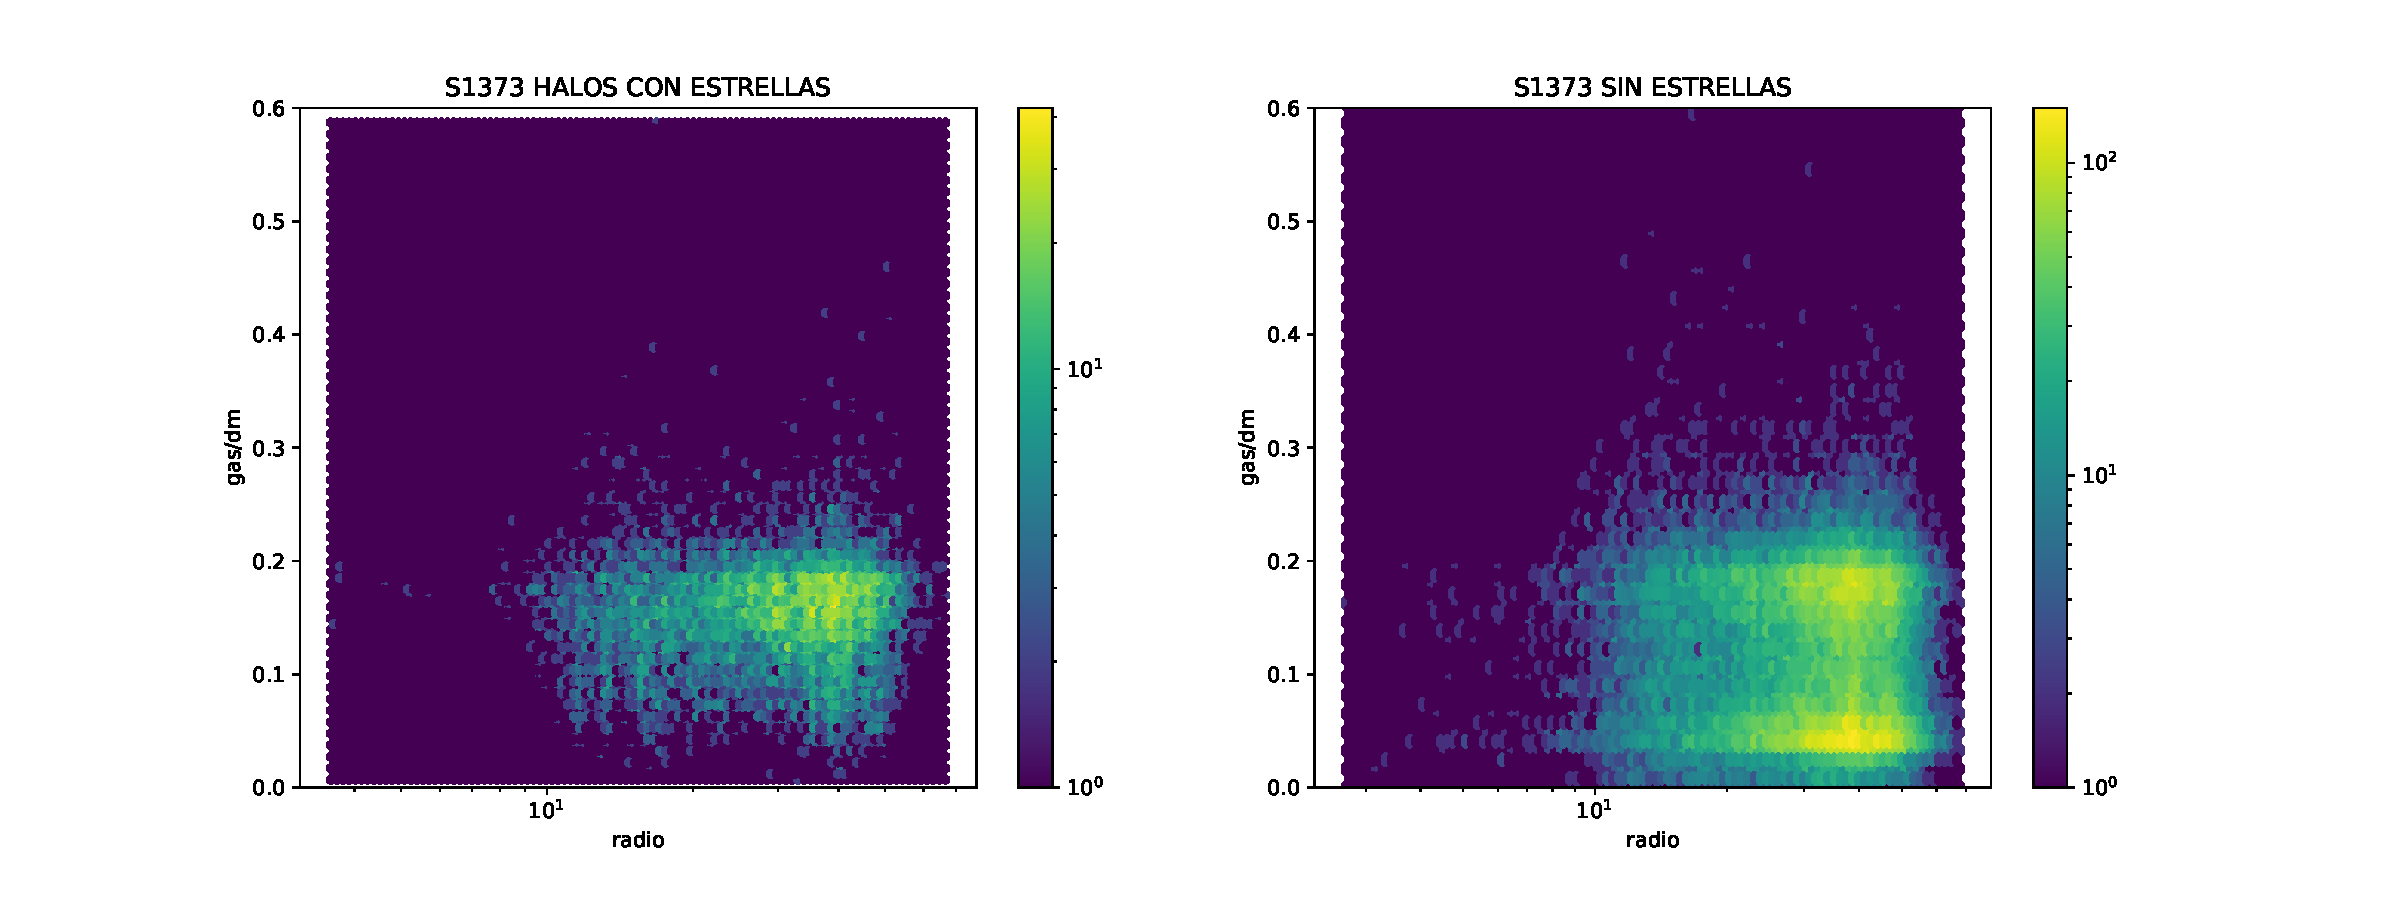
\includegraphics[width=18cm]{Figures/S1373_scatterFRACCIONES_con&sinEST.pdf}
\decoRule
\caption[R1198 GAS/DM perfil (scatter) con y sin estrellas]{Perfil de gas/dm para los halos. A  la izquierda estan los halos que contienen al menos una particula de estrellas. A la derehc a los que no tienen ninguna estrella}
\label{fig:Electron}
\end{figure}

\begin{figure}[h]
\centering
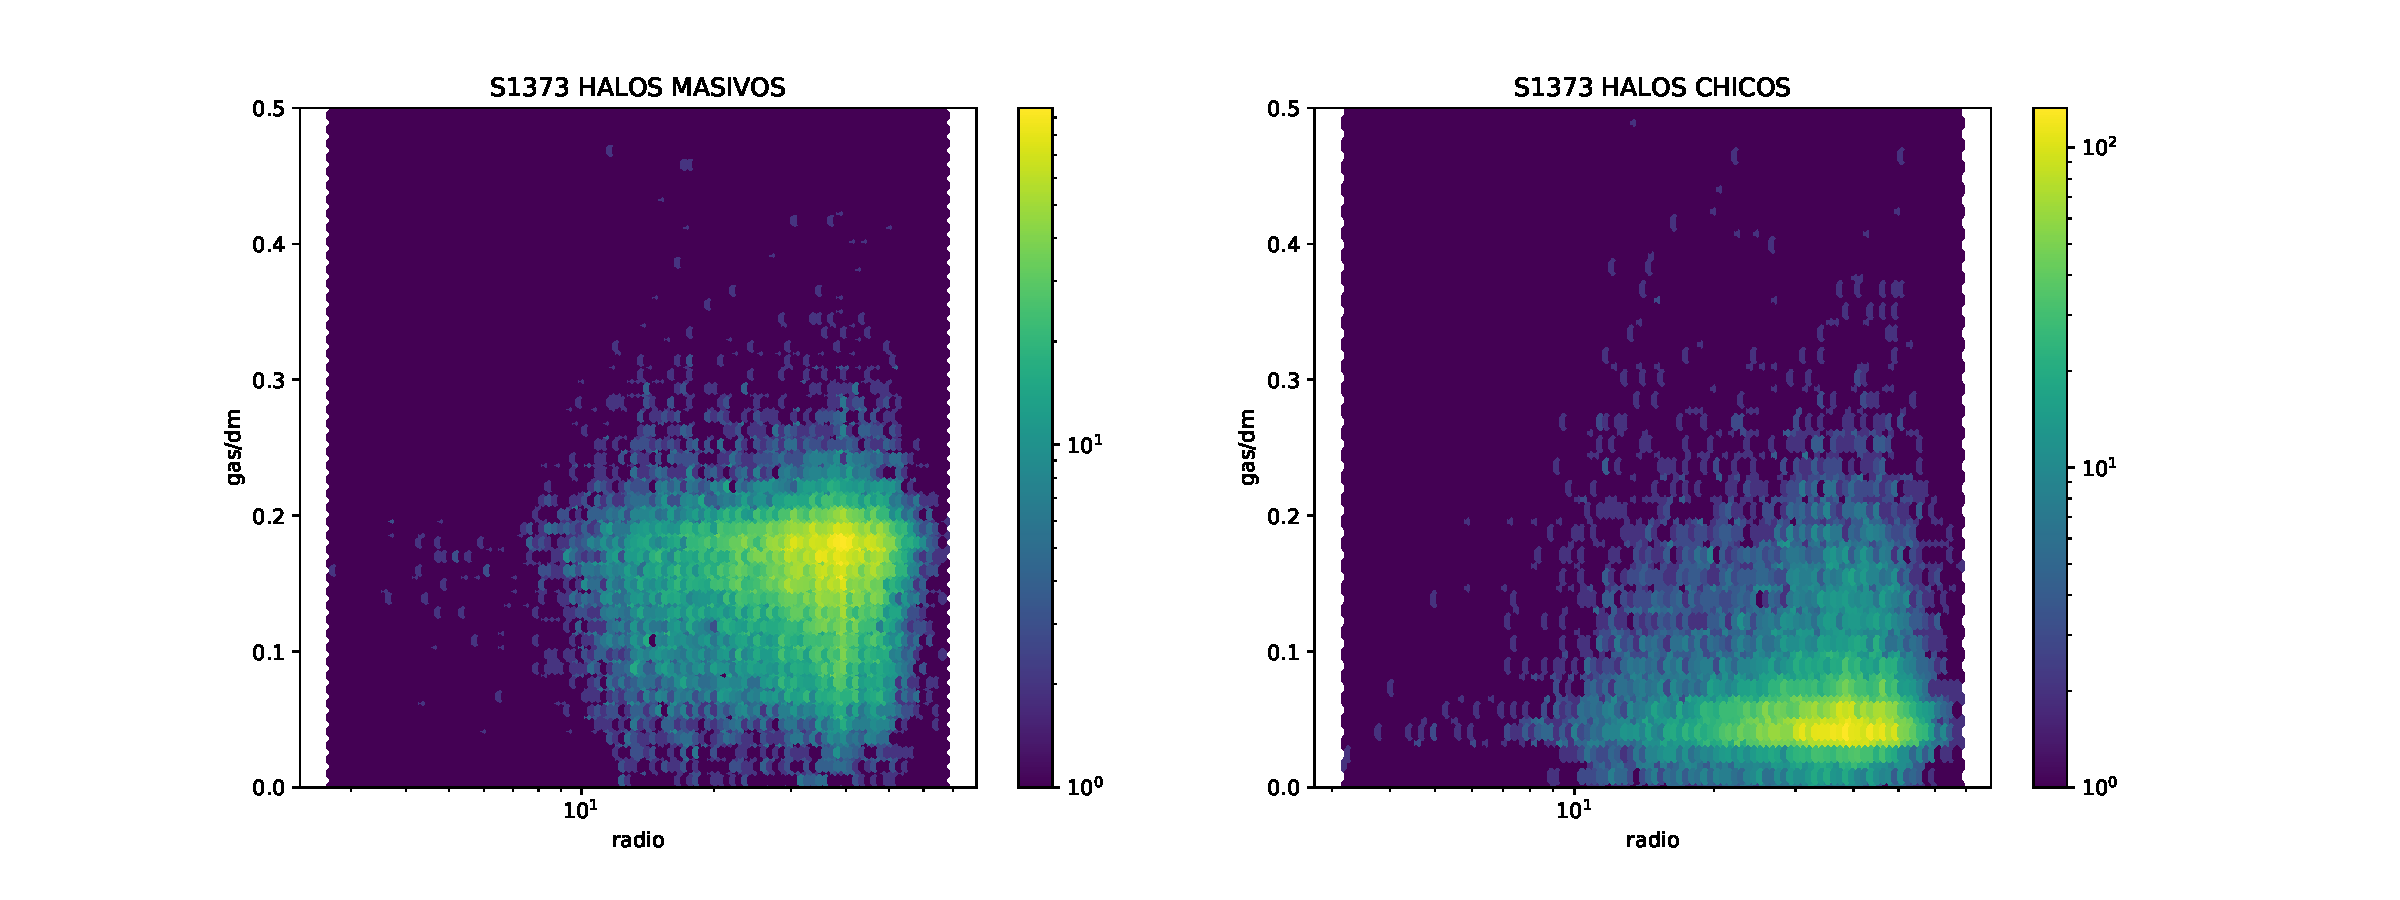
\includegraphics[width=18cm]{Figures/S1373_scatterFRACCIONES_grandesYchicos.pdf}
\decoRule
\caption[R1198 GAS/DM perfil (scatter) halos grandes y chicos]{fraccion de gas sobre DM separando los halos por tamaño. Los halos GRANDES tienen mas de 50 particulas de DM, los chicos menos de 50. }
\label{fig:Electron}
\end{figure}


%% Chapter 1

\chapter{DIAGRAMAS DE FASE} % Main chapter title

(paper Shuiyao Huang et al. 2019) 



Most of these
gas particles lie on a well-defined curve in the phase diagram,
which is established by a balance between adiabatic cooling and photoionization heating. A fraction of gas particles are shock heated
when they collapse into the gravitational potential of dark matter
sheets and filaments and are driven into warm-and-hot ionized gas
outside of haloes (upper left) or fall into dark matter haloes and
become hot halo gas (upper right). Radiative cooling later plays a
critical role in the further condensation of gas into the condensed
region (lower right) where SF can occur. In addition, some gas goes
straight from the diffuse to the condensed region, i.e. cold mode
accretion (Keres et al. ˇ 2005, 2009a).



Calcule las fracciones al estilo de Martizzi 2009 y me dio, corte en dens = 2.5 y temp = 5 (la temperatura es el mismo corte, la densidad lo meti a ojo) Me dan muy diferentes. ESTO ES PARA EL VOID S
\begin{figure}[h]
\centering
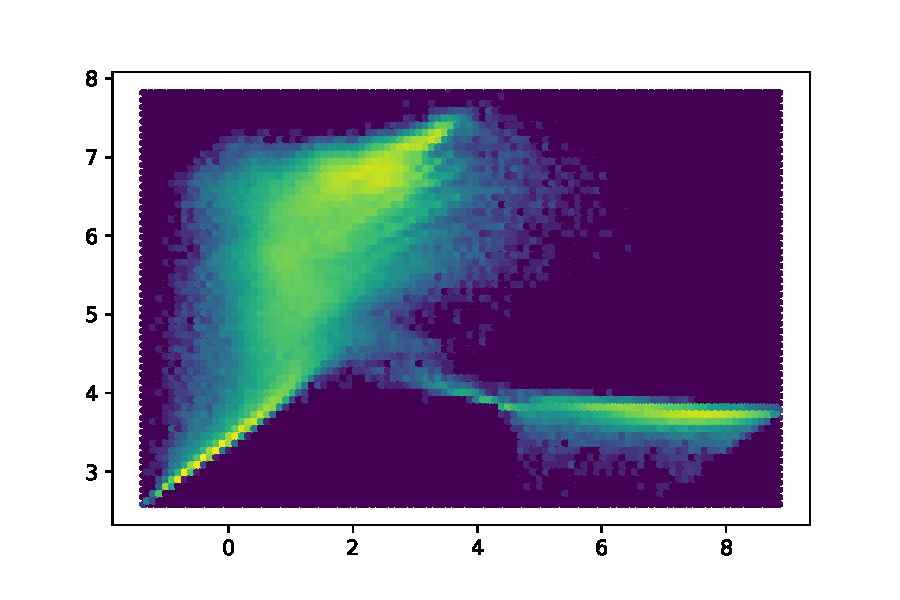
\includegraphics[width=14cm]{Figures/S1373_diagfaseVOID.pdf}
\decoRule
\caption[Diagrama de Fase TODAS particulas]{Densidad vs Temperatura considerando las particulas del void r<9.75}
\label{fig:Electron}
\end{figure}


fraccion DIF 0.19707932560856978

fraccion HALO 0.13583764565477252

fraccion WHIM 0.49660098890788423

fraccion WCGM 0.1704743649519073

fraccion SF 7.674876866194279e-06
\label{Chapter2} % For referencing the chapter elsewhere, use \ref{Chapter1} 

%----------------------------------------------------------------------------------------

% Define some commands to keep the formatting separated from the content 

%----------------------------------------------------------------------------------------
\section{R1198}

\begin{figure}[h]
\centering
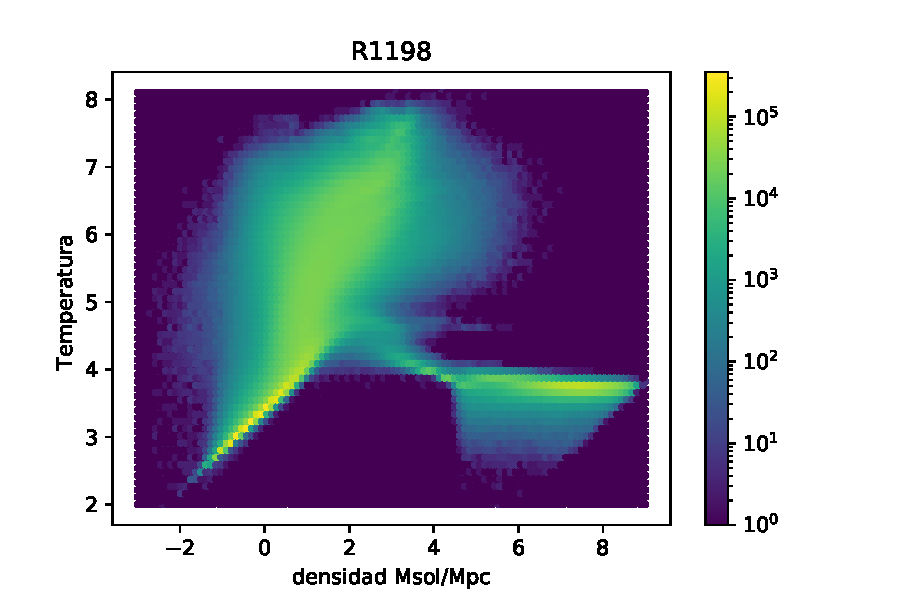
\includegraphics[width=18cm]{Figures/R1198_diagfase.pdf}
\decoRule
\caption[Diagrama de Fase TODAS particulas]{Densidad vs Temperatura considerando todas las particulas $\sim$ 33 millones}
\label{fig:Electron}
\end{figure}

\begin{figure}[h]
\centering
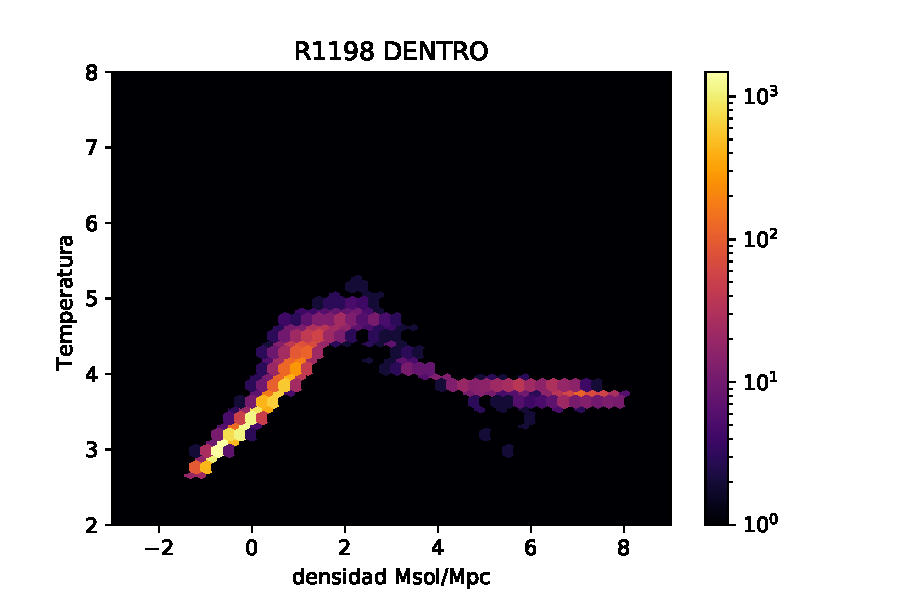
\includegraphics[width=18cm]{Figures/R1198_diagfase_int.pdf}
\decoRule
\caption[Diagrama de Fase R internas]{particulas dentro de un radio de 6 mpc}
\label{fig:Electron}
\end{figure}
\begin{figure}[h]
\centering
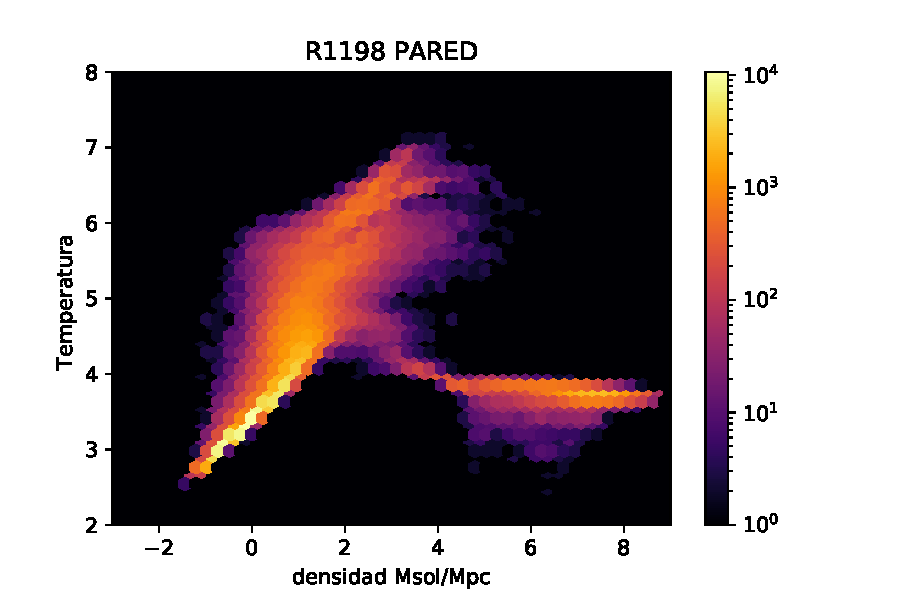
\includegraphics[width=18cm]{Figures/R1198_diagfase_wll.pdf}
\decoRule
\caption[Diagrama de Fase R pared]{particulas entre 6 y 12 Mpc}
\label{fig:Electron}
\end{figure}
\begin{figure}[h]
\centering
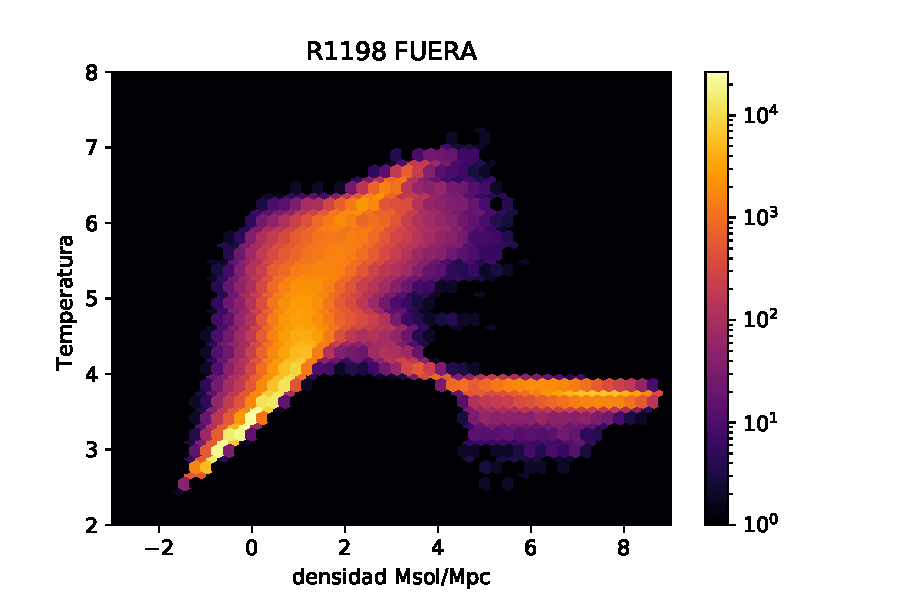
\includegraphics[width=18cm]{Figures/R1198_diagfase_ext.pdf}
\decoRule
\caption[Diagrama de Fase R externas]{particulas entre 12 y 18 Mpc}
\label{fig:Electron}
\end{figure}




\section{S1373}

\begin{figure}[h]
\centering
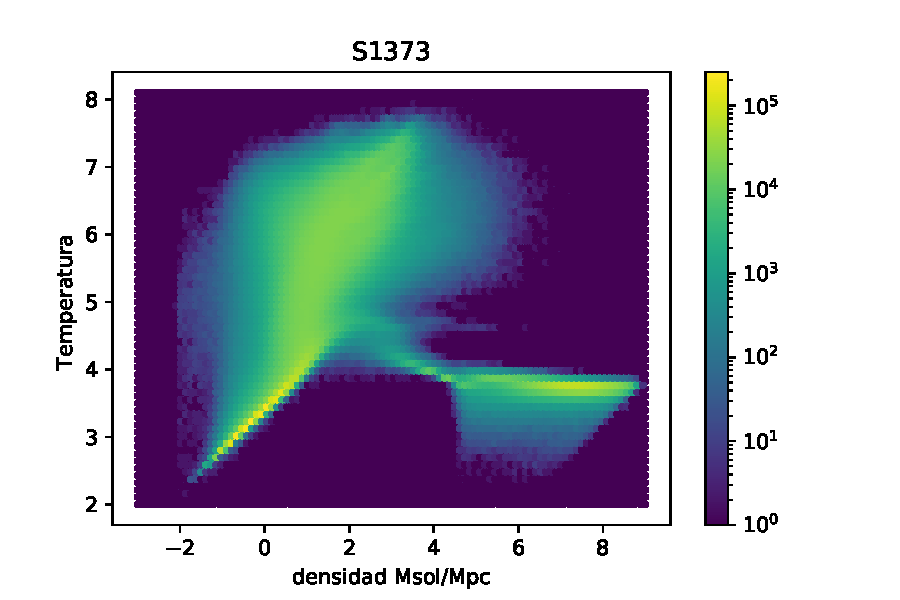
\includegraphics[width=18cm]{Figures/S1373_diagfase.pdf}
\decoRule
\caption[Diagrama de Fase TODAS particulas]{Densidad vs Temperatura considerando todas las particulas $\sim$ 33 millones}
\label{fig:Electron}
\end{figure}



\begin{figure}[h]
\centering
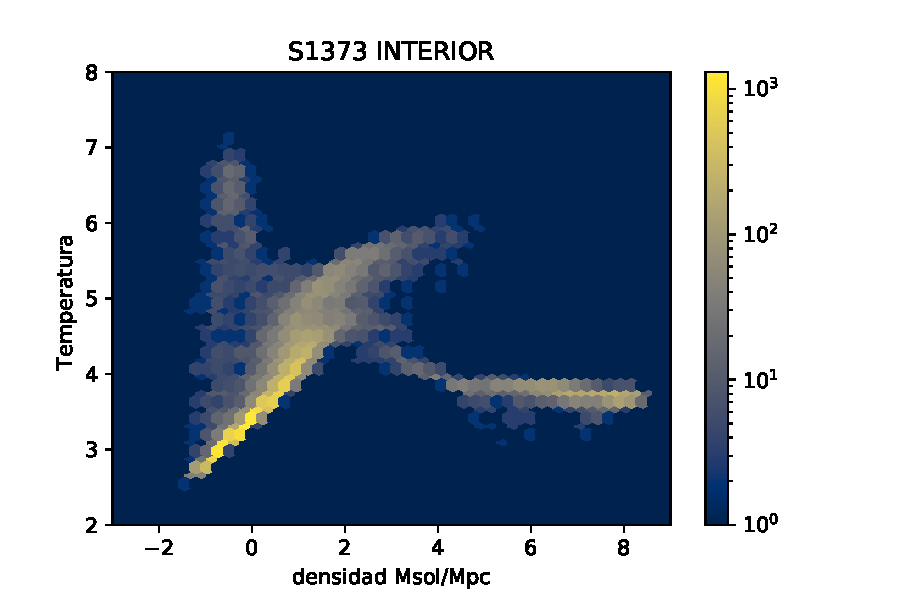
\includegraphics[width=18cm]{Figures/S1373_diagfase_int.pdf}
\decoRule
\caption[Diagrama de Fase S internas]{particulas dentro de un radio de 6 mpc}
\label{fig:Electron}
\end{figure}
\begin{figure}[h]
\centering
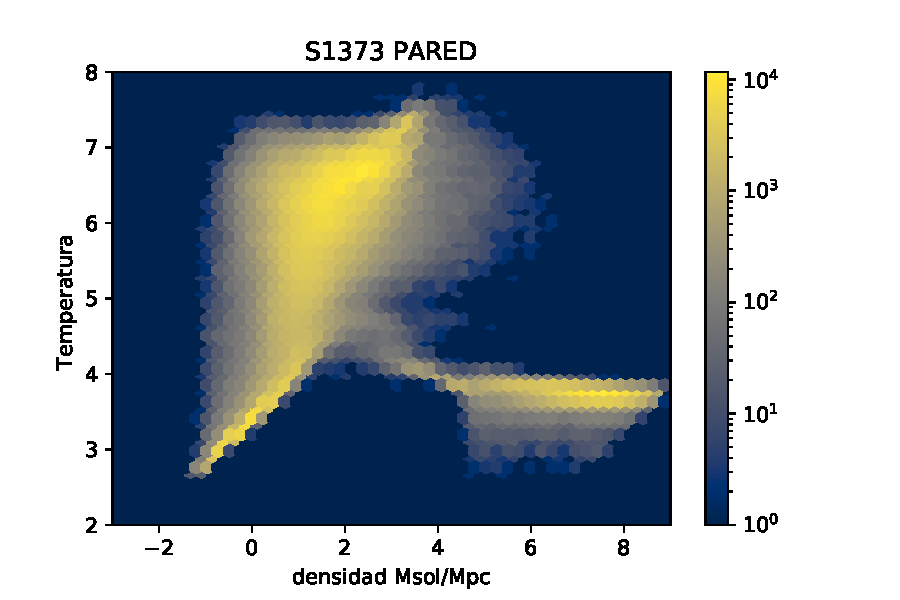
\includegraphics[width=18cm]{Figures/S1373_diagfase_wll.pdf}
\decoRule
\caption[Diagrama de Fase S pared]{particulas entre 6 y 12 Mpc}
\label{fig:Electron}
\end{figure}
\begin{figure}[h]
\centering
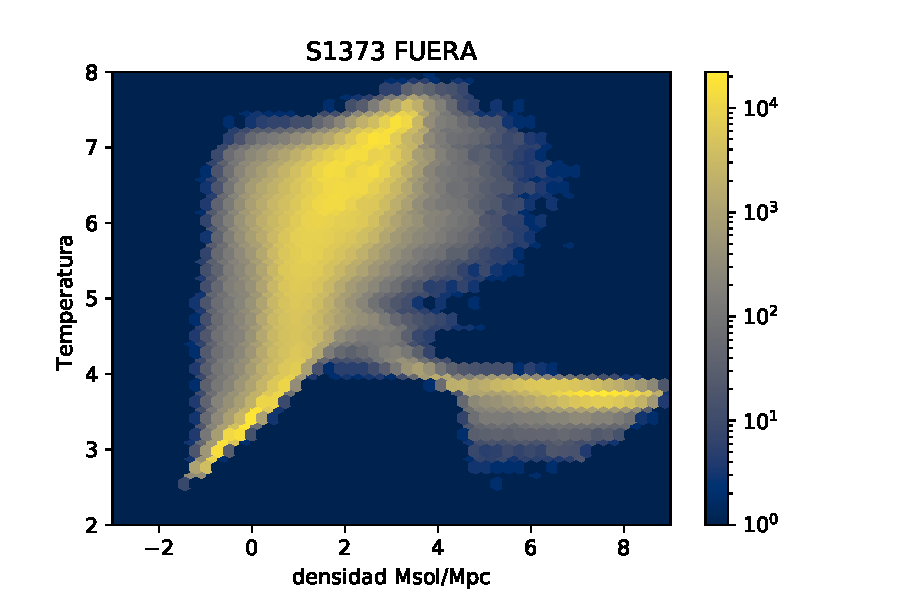
\includegraphics[width=18cm]{Figures/S1373_diagfase_ext.pdf}
\decoRule
\caption[Diagrama de Fase S externas]{particulas entre 12 y 18 Mpc}
\label{fig:Electron}
\end{figure} 
%\chapter{look back time}

Agarre el Void S mas alla de el radio de void (15 < r > 25) donde la densidad es mas parecida que a la del universo  e hice los diagramas de fase a diferentes redshift. 

\begin{figure}[h]
\centering
\includegraphics[width=18cm]{Figures/S_df_s25.pdf}
\decoRule
\caption[Fraccione stellar vs gas]{Fracciones de gs/dm vs estrellas/dm }
\label{fig:Electron}
\end{figure}

\begin{figure}[h]
\centering
\includegraphics[width=18cm]{Figures/S_df_s20.pdf}
\decoRule
\caption[Fraccione stellar vs gas]{Fracciones de gs/dm vs estrellas/dm }
\label{fig:Electron}
\end{figure}

\begin{figure}[h]
\centering
\includegraphics[width=18cm]{Figures/S_df_s15.pdf}
\decoRule
\caption[Fraccione stellar vs gas]{Fracciones de gs/dm vs estrellas/dm }
\label{fig:Electron}
\end{figure}
%\chapter{4}


\begin{figure}[h]
\centering
\includegraphics[width=18cm]{Figures/R1198_gas-est_frac.pdf}
\decoRule
\caption[Fraccione stellar vs gas]{Fracciones de gs/dm vs estrellas/dm }
\label{fig:Electron}
\end{figure}

\begin{figure}[h]
\centering
\includegraphics[width=18cm]{Figures/S1373_gas-est_frac.pdf}
\decoRule
\caption[Fraccione stellar vs gas]{Fracciones de gs/dm vs estrellas/dm }
\label{fig:Electron}
\end{figure}

\begin{figure}[h]
\centering
\includegraphics[width=18cm]{Figures/S1373_fraccionesdebarions.pdf}
\decoRule
\caption[Fraccione stellar vs gas]{Fracciones de gs/dm vs estrellas/dm para el VOID (r<10 Mpc y para el entorno r>10}
\label{fig:Electron}
\end{figure}

\begin{figure}[h]
\centering
\includegraphics[width=18cm]{Figures/R1198_frac-spin.pdf}
\decoRule
\caption[Fraccione stellar vs gas]{Fracciones de gs/dm vs estrellas/dm para el VOID (r<10 Mpc y para el entorno r>10}
\label{fig:Electron}
\end{figure}

\begin{figure}[h]
\centering
\includegraphics[width=18cm]{Figures/SF.pdf}
\decoRule
\caption[Fraccione stellar vs gas]{Fracciones de gs/dm vs estrellas/dm para el VOID (r<10 Mpc y para el entorno r>10}
\label{fig:Electron}
\end{figure}

\begin{figure}[h]
\centering
\includegraphics[width=18cm]{Figures/ESTRELLAS.pdf}
\decoRule
\caption[Fraccione stellar vs gas]{Fracciones de gs/dm vs estrellas/dm para el VOID (r<10 Mpc y para el entorno r>10}
\label{fig:Electron}
\end{figure}

\begin{figure}[h]
\centering
\includegraphics[width=18cm]{Figures/GAS.pdf}
\decoRule
\caption[Fraccione stellar vs gas]{Fracciones de gs/dm vs estrellas/dm para el VOID (r<10 Mpc y para el entorno r>10}
\label{fig:Electron}
\end{figure}

\begin{figure}[h]
\centering
\includegraphics[width=18cm]{Figures/R1198_SFhist.pdf}
\decoRule
\caption[R1198 SF distribucion]{histograma de las 245 particulas de gas con formaci\'on estelar}
\label{fig:Electron}
\end{figure}

\begin{figure}[h]
\centering
\includegraphics[width=18cm]{Figures/S1373_SFhist.pdf}
\decoRule
\caption[S1373 SF distribucion]{histograma de las 205 particulas de gas con formaci\'on estelar}
\label{fig:Electron}
\end{figure} 
%\chapter{5}

\begin{figure}[h]
\centering
\includegraphics[width=10cm]{Figures/RSF_history.pdf}
\decoRule
\caption[RSF hsitory]{perfil diferencial de formacion estelar a diferentes redshift}
\label{fig:Electron}
\end{figure}

\begin{figure}[h]
\centering
\includegraphics[width=10cm]{Figures/SSF_history.pdf}
\decoRule
\caption[SSF hsitory]{perfil diferencial de formacion estelar a diferentes redshift}
\label{fig:Electron}
\end{figure}

\begin{figure}[h]
\centering
\includegraphics[width=18cm]{Figures/R_sctFRACC1.pdf}
\decoRule
\caption[perfil del void R]{}
\label{fig:Electron}
\end{figure}

\begin{figure}[h]
\centering
\includegraphics[width=18cm]{Figures/R_sctFRACC2.pdf}
\decoRule
\caption[perfil del void R]{}
\label{fig:Electron}
\end{figure}

\begin{figure}[h]
\centering
\includegraphics[width=18cm]{Figures/R_sctFRACC3.pdf}
\decoRule
\caption[perfil del void R]{}
\label{fig:Electron}
\end{figure}

\begin{figure}[h]
\centering
\includegraphics[width=18cm]{Figures/R_sctFRACC4.pdf}
\decoRule
\caption[perfil del void R]{}
\label{fig:Electron}
\end{figure}


\begin{figure}[h]
\centering
\includegraphics[width=18cm]{Figures/S_sctFRACC1.pdf}
\decoRule
\caption[perfil del void R]{}
\label{fig:Electron}
\end{figure}
\begin{figure}[h]
\centering
\includegraphics[width=18cm]{Figures/S_sctFRACC2.pdf}
\decoRule
\caption[perfil del void R]{}
\label{fig:Electron}
\end{figure}
\begin{figure}[h]
\centering
\includegraphics[width=18cm]{Figures/S_sctFRACC3.pdf}
\decoRule
\caption[perfil del void R]{}
\label{fig:Electron}
\end{figure}
\begin{figure}[h]
\centering
\includegraphics[width=18cm]{Figures/S_sctFRACC4.pdf}
\decoRule
\caption[perfil del void R]{}
\label{fig:Electron}
\end{figure}



\begin{figure}[h]
\centering
\includegraphics[width=10cm]{Figures/S_hsml.pdf}
\decoRule
\caption[asd]{VOID S distribucion para los maximo hsml/radio virial }
\label{fig:Electron}
\end{figure}

\begin{figure}[h]
\centering
\includegraphics[width=10cm]{Figures/R_hsml.pdf}
\decoRule
\caption[asd]{VOID R distribucion para los maximo hsml/radio virial }
\label{fig:Electron}
\end{figure}

\begin{figure}[h]
\centering
\includegraphics[width=18cm]{Figures/R_control1.pdf}
\decoRule
\caption[asd]{VOID R distribucion para los maximo hsml/radio virial }
\label{fig:Electron}
\end{figure}

\begin{figure}[h]
\centering
\includegraphics[width=15cm]{Figures/R1198_DF1.pdf}
\decoRule
\caption[asd]{diagramas de fase para el void R1198}
\label{fig:Electron}
\end{figure}

\begin{figure}[h]
\centering
\includegraphics[width=15cm]{Figures/S1373_DF1.pdf}
\decoRule
\caption[asd]{diagramas de fase para el void S}
\label{fig:Electron}
\end{figure}

\begin{figure}[h]
\centering
\includegraphics[width=15cm]{Figures/R1198_sph1.pdf}
\decoRule
\caption[asd]{diagramas de fase para el void S}
\label{fig:Electron}
\end{figure}

\begin{figure}[h]
\centering
\includegraphics[width=15cm]{Figures/S1373_sph1.pdf}
\decoRule
\caption[asd]{diagramas de fase para el void S}
\label{fig:Electron}
\end{figure}

\begin{figure}[h]
\centering
\includegraphics[width=15cm]{Figures/S1373_sph2.pdf}
\decoRule
\caption[asd]{diagramas de fase para el void S}
\label{fig:Electron}
\end{figure}

\begin{figure}[h]
\centering
\includegraphics[width=15cm]{Figures/S1373_sph3.pdf}
\decoRule
\caption[asd]{Perfil de densidad diferencial para el void S. Se promediaron 200 muestras cada 10. }
\label{fig:Electron}
\end{figure}

\begin{figure}[h]
\centering
\includegraphics[width=15cm]{Figures/R1198_sph3.pdf}
\decoRule
\caption[asd]{Perfil de densidad diferencial para el void R. Se promediaron 200 muestras cada 10. }
\label{fig:Electron}
\end{figure}

\begin{figure}[h]
\centering
\includegraphics[width=15cm]{Figures/R1198_zoomin1.pdf}
\decoRule
\caption[asd]{resimulacion del void R }
\label{fig:Electron}
\end{figure}

\begin{figure}[h]
\centering
\includegraphics[width=15cm]{Figures/S1373_zoomin1.pdf}
\decoRule
\caption[asd]{resiumacion del void S }
\label{fig:Electron}
\end{figure} 
%\chapter*{Chapter6}

\label{PostSemi}


\begin{figure}[h]
\centering
\includegraphics[width=10cm]{Figures/fracciones_R.png}
\decoRule
\caption[asd]{VOID R: esto es en sextiles  }
\label{fig:Electron}
\end{figure}
\begin{figure}[h]
\centering
\includegraphics[width=10cm]{Figures/histogramas_R.png}
\decoRule
\caption[asd]{VOID R: SEXTILES  }
\label{fig:Electron}
\end{figure}

\begin{figure}[h]
\centering
\includegraphics[width=10cm]{Figures/fracciones_S.png}
\decoRule
\caption[asd]{VOID S SEXTILES  }
\label{fig:Electron}
\end{figure}
\begin{figure}[h]
\centering
\includegraphics[width=10cm]{Figures/histogramas_S.png}
\decoRule
\caption[asd]{VOID S  SEXTILES}
\label{fig:Electron}
\end{figure}

\begin{figure}[h]
\centering
\includegraphics[width=10cm]{Figures/DFprof_S.png}
\decoRule
\caption[asd]{VOID S  estos son intervalos de delta integrada, -1/-0.8; -0.8/-0.6, etc.. hasta 0. El numero de arriba de los plots es la distancia al centro del void.}
\label{fig:Electron}
\end{figure}


\begin{figure}[h]
\centering
\includegraphics[width=10cm]{Figures/DFprof_R.png}
\decoRule
\caption[asd]{VOID R estos son intervalos de delta integrada, -1/-0.8; -0.8/-0.6, etc.. hasta 0. El numero de arriba de los plots es la distancia al centro del void. }
\label{fig:Electron}
\end{figure}

\begin{figure}[h]
\centering
\includegraphics[width=10cm]{Figures/DF_wallS.png}
\decoRule
\caption[asd]{VOID S: esto es entre 5<r<11. El numero de arriba del plot es el redshit  }
\label{fig:Electron}
\end{figure}

\begin{figure}[h]
\centering
\includegraphics[width=10cm]{Figures/DF_inS.png}
\decoRule
\caption[asd]{VOID S: esto es para r<5  El numero de arriba del plot es el redshit    }
\label{fig:Electron}
\end{figure}

\begin{figure}[h]
\centering
\includegraphics[width=10cm]{Figures/DF_wallR.png}
\decoRule
\caption[asd]{VOID R: esto es entre 5<r<11  El numero de arriba del plot es el redshit   }
\label{fig:Electron}
\end{figure}

\begin{figure}[h]
\centering
\includegraphics[width=10cm]{Figures/DF_inR.png}
\decoRule
\caption[asd]{VOID R: esto es para r<5  El numero de arriba del plot es el redshit   }
\label{fig:Electron}
\end{figure}

\begin{figure}[h]
\centering
\includegraphics[width=10cm]{Figures/fraccionesDelta_S.png}
\decoRule
\caption[asd]{VOID S, las fracciones son para los halos que tienen estrellas. Cada plot es un intervalo de delta integrada }
\label{fig:Electron}
\end{figure}

\begin{figure}[h]
\centering
\includegraphics[width=10cm]{Figures/fraccionesDelta_R.png}
\decoRule
\caption[asd]{VOID R: halos con estrellas. Cada plot es un intervalo de delta integrada }
\label{fig:Electron}
\end{figure}

\begin{figure}[h]
\centering
\includegraphics[width=10cm]{Figures/FasesProf_R.png}
\decoRule
\caption[asd]{VOID R. Estos son particulas/vol.  }
\label{fig:Electron}
\end{figure}

\begin{figure}[h]
\centering
\includegraphics[width=10cm]{Figures/ProfFases_R.png}
\decoRule
\caption[asd]{VOID R: Con jacknife, con 48 realizaciones,500 mediciones y promedios cada 20 }
\label{fig:Electron}
\end{figure}

\begin{figure}[h]
\centering
\includegraphics[width=10cm]{Figures/FasesProf_S.png}
\decoRule
\caption[asd]{VOID S , p articulas/volumen}
\label{fig:Electron}
\end{figure}

\begin{figure}[h]
\centering
\includegraphics[width=10cm]{Figures/ProfFases_S.png}
\decoRule
\caption[asd]{VOID S: Con jacknife, con 48 realizaciones, 500 mediciones y promedios cada 20. }
\label{fig:Electron}
\end{figure}





\begin{figure}[h]
\centering
\includegraphics[width=10cm]{Figures/FasesHexbin_S.png}
\decoRule
\caption[asd]{VOID S, es un corte transversal de 4 Mpc de profundidad que pasa por el centro del void }
\label{fig:Electron}
\end{figure}

\begin{figure}[h]
\centering
\includegraphics[width=10cm]{Figures/FasesHexbin_R.png}
\decoRule
\caption[asd]{VOID R, es un corte transversal de 4 Mpc de profundidad que pasa por el centro del void }
\label{fig:Electron}
\end{figure}
%\chapter*{Chapter7}


Teniendo en cuenta que los voids fueron identificados en halos de 20 particulas, me fije cual es la masa minima que corresponde a esos halos ($M\sim 71$), entonces estos tienen una masa minima de $\sim 140 \hspace{1}[10^{10}M_{\odot}]$, pero una fracci\'on de 0.18 de esa masa es bariones y el resto es DM, entonces la masa de materia oscura de esos halos es 116, y en la resimulacion se corresponde a halos que tengan al menos 1231 particulas de materia oscura. Entonces hice los perfiles de halos con un corte en 1231 particulas para elegir donde cortar entre adentro y afuera. 

Elegi  $\Delta=-0.7$ para hacer el corte, porque si ponia menos me quedaban muy pocos halos. Eso se corresponde de un radio de $R_{S}=10\hspace{1}Mpc$ y $R_{R}=13$. Y la regi\'on de fuera del void es $R_{S}=25-30$ que es donde $\Delta\sim0$. 

Para hacer los cortes por masa, primero hice un corte inferior en elegir halos que tengan al menos 60 particulas de gas (con la idea esa de que un halo con esa cantidad de particulas esta bien resuelto) y despues elegi los rangos de 60-120 y 120-1000. (la idea era cortar en 100 pero me quedan pocos halos). Los cortes en 120 y 1000 son mirando las particulas de materia oscura. 
Entonces me terminan quedando:
menos de 120 particulas:

48 halos void S

111 halos void R

entre 120-1000 particulas:

126 halos void S

136 halos void R

\begin{figure}[h]
\centering
\includegraphics[width=10cm]{Figures/Fraccion_cortemasa.png}
\decoRule
\caption[asd]{Estas son las fracciones de masa de los halos, mirando el gas. Ahi puede haber algo con el void S, aunque son pocos halos :/}
\label{fig:Electron}
\end{figure}

\begin{figure}[h]
\centering
\includegraphics[width=10cm]{Figures/Densidades_cortemasa.png}
\decoRule
\caption[asd]{Estas son las densidades, estoy tomando particulas a dos radios viriales,entonces seria la masa de particulas dividido 2 radios viriales.  }
\label{fig:Electron}
\end{figure}

\begin{figure}[h]
\centering
\includegraphics[width=10cm]{Figures/Spin_cortemasa.png}
\decoRule
\caption[asd]{Aca mire el spin de los halos, pero es solamente el spin que me tira rockstar  }
\label{fig:Electron}
\end{figure}

\begin{figure}[h]
\centering
\includegraphics[width=10cm]{Figures/Momangular_cortemasa.png}
\decoRule
\caption[asd]{Aca tengo el modulo del momento angular (con las componentes que me tira rockstar) dividido el numero de particulas, donde estas particulas son tambien las que rockstar dice que tiene cada halo }
\label{fig:Electron}
\end{figure}

\begin{figure}[h]
\centering
\includegraphics[width=10cm]{Figures/temperatura_cortemasa.png}
\decoRule
\caption[asd]{Y este tiene las temperaturas de los halos, el codigo de colores es el mismo que los plots anteriores y en el label lo que esta es la mediana de la temperatura, si pongo la promedio me da valores muy extremos, me queda a la izquierda : 4.7e4 K para los voids y 2.7e5 para fuera del void, derecha: 1.3e5 void S, 1.7e5 void R y 6e5 afuera}
\label{fig:Electron}
\end{figure}

%----------------------------------------------------------------------------------------
%	THESIS CONTENT - APPENDICES
%----------------------------------------------------------------------------------------

\appendix % Cue to tell LaTeX that the following "chapters" are Appendices

% Include the appendices of the thesis as separate files from the Appendices folder
% Uncomment the lines as you write the Appendices


\chapter{Simulaciones utilizadas} % Main appendix title

\label{Apendice} % For referencing this appendix elsewhere, use \ref{AppendixA}

\begin{table}[ht]
\begin{tabular}{c|c|c|c|c|c}
    - & n_{dm} & n_{gs}  &  m_{dm}   & m_{gs}   & box [Mpc] \\
\hline    Base     & 500^{3}  & -  & &  &  500   \\
\hline    Void S   & 3.0 10^{7}   &  3.0 10^{7} & 9.3 10^{8} &1.8 10^{8} & 80    \\
\hline    Void R   & 3.6 10^{7}   & 3.6 10^{7}   &9.3 10^{8} & 1.8 10^{8} & 80  \\
\hline    Ref      & 9.8   & 10.1  & 9.3 10^{8}    &1.8 10^{8} & 120 \\
\hline
\end{tabular}
\caption{..}
\label{Simulaciones0}
\end{table}

\begin{figure}
    \centering
    \includegraphics[width=13cm]{Figures/Spin_cortemasa.png}
    \caption{Caption}
    \label{fig:my_label}
\end{figure}{}
%\include{Appendices/AppendixB}
%\include{Appendices/AppendixC}

%----------------------------------------------------------------------------------------
%	BIBLIOGRAPHY
%----------------------------------------------------------------------------------------

\printbibliography[heading=bibintoc]

%----------------------------------------------------------------------------------------

\end{document}  
